% =============================================================================
%  web-audit.tex — ผลตรวจความถูกต้อง ความสมเหตุสมผล และความสอดคล้องของเว็บ ULMs
%  รวมคำวินิจฉัยข้อคิดเห็นของ dev (15 ก.ย. 2569) เทียบกับแผนงาน
%
%  ต้องคอมไพล์ด้วย XeLaTeX:   cd docs && latexmk web-audit.tex  → build/web-audit.pdf
%                             แล้ว cp build/web-audit.pdf report/
%
%  ตรวจบน origin/main = b1bca77 (14 ก.ย. 2569) · ฐานข้อมูล ulms_audit ที่ seed ใหม่
%
%  ที่มาของตัวเลขและรูปทุกชิ้น (ถ้ารันซ้ำแล้วค่าเปลี่ยน เนื้อความต้องตามไปแก้):
%    docs/audit/api_scenarios.py   → docs/audit/results/s1_counters.json ... s5_registration.json
%    docs/audit/capture_screens.py → docs/figures/audit/*.jpg + docs/audit/results/screens.json
%    docs/audit/results/fr_list.json  FR 86 ข้อ ดึงจาก docs/specs/srs_data.py
%    ภาพหน้าจอทุกภาพ 1440x900 px — ค่า trim ของ \includegraphics คิดจากขนาดนี้
%  ลำดับรันที่ถูก: reset ฐาน → capture_screens.py → api_scenarios.py
%  (ถ้ารันสลับ ของทดสอบชื่อ AUDIT-* จะไปโผล่ในภาพหน้ารายการครุภัณฑ์)
% =============================================================================

% =============================================================================
%  trpc-preamble.tex — preamble ร่วมของเอกสารชุด "สัญญา tRPC" ของโครงการ ULMs
%
%  ใช้โดย:  trpc-guide.tex    (ฉบับที่ 1 — หลักการ tRPC + ความเสี่ยงใน repo นี้)
%           trpc-meeting.tex  (ฉบับที่ 2 — วาระประชุมเรียงตามลำดับความสำคัญ)
%
%  ทำไมไม่ใช้ ulms-preamble.tex ที่มีอยู่แล้ว
%  ----------------------------------------
%  ulms-preamble.tex ตั้งใจให้เป็น "โทนเดียว (monochrome)" สำหรับเอกสารที่ต้อง
%  ส่งอาจารย์/พิมพ์ขาวดำ แต่เอกสารสอนสองฉบับนี้ใช้ "สีเชิงความหมาย" เป็นเครื่องมือ
%  สอนหลัก (สีเดียวกัน = แนวคิดเดียวกัน ทั้งในเนื้อความ ในไดอะแกรม และในตาราง)
%  จึงต้องมี preamble ของตัวเอง — ไม่ใช่ก๊อปมาแก้สีทับ
%
%  เอกสารที่เรียกใช้ต้องทำสองอย่างหลัง % =============================================================================
%  trpc-preamble.tex — preamble ร่วมของเอกสารชุด "สัญญา tRPC" ของโครงการ ULMs
%
%  ใช้โดย:  trpc-guide.tex    (ฉบับที่ 1 — หลักการ tRPC + ความเสี่ยงใน repo นี้)
%           trpc-meeting.tex  (ฉบับที่ 2 — วาระประชุมเรียงตามลำดับความสำคัญ)
%
%  ทำไมไม่ใช้ ulms-preamble.tex ที่มีอยู่แล้ว
%  ----------------------------------------
%  ulms-preamble.tex ตั้งใจให้เป็น "โทนเดียว (monochrome)" สำหรับเอกสารที่ต้อง
%  ส่งอาจารย์/พิมพ์ขาวดำ แต่เอกสารสอนสองฉบับนี้ใช้ "สีเชิงความหมาย" เป็นเครื่องมือ
%  สอนหลัก (สีเดียวกัน = แนวคิดเดียวกัน ทั้งในเนื้อความ ในไดอะแกรม และในตาราง)
%  จึงต้องมี preamble ของตัวเอง — ไม่ใช่ก๊อปมาแก้สีทับ
%
%  เอกสารที่เรียกใช้ต้องทำสองอย่างหลัง % =============================================================================
%  trpc-preamble.tex — preamble ร่วมของเอกสารชุด "สัญญา tRPC" ของโครงการ ULMs
%
%  ใช้โดย:  trpc-guide.tex    (ฉบับที่ 1 — หลักการ tRPC + ความเสี่ยงใน repo นี้)
%           trpc-meeting.tex  (ฉบับที่ 2 — วาระประชุมเรียงตามลำดับความสำคัญ)
%
%  ทำไมไม่ใช้ ulms-preamble.tex ที่มีอยู่แล้ว
%  ----------------------------------------
%  ulms-preamble.tex ตั้งใจให้เป็น "โทนเดียว (monochrome)" สำหรับเอกสารที่ต้อง
%  ส่งอาจารย์/พิมพ์ขาวดำ แต่เอกสารสอนสองฉบับนี้ใช้ "สีเชิงความหมาย" เป็นเครื่องมือ
%  สอนหลัก (สีเดียวกัน = แนวคิดเดียวกัน ทั้งในเนื้อความ ในไดอะแกรม และในตาราง)
%  จึงต้องมี preamble ของตัวเอง — ไม่ใช่ก๊อปมาแก้สีทับ
%
%  เอกสารที่เรียกใช้ต้องทำสองอย่างหลัง \input{trpc-preamble}:
%    1) \hypersetup{pdftitle={...}}
%    2) \begin{document}
%
%  Build:  cd docs && latexmk trpc-guide.tex     (.latexmkrc บังคับ xelatex ให้แล้ว)
%          PDF ออกที่ docs/build/ แล้วค่อยคัดลอกไป docs/report/
% =============================================================================

\documentclass[11pt,a4paper]{article}

% ---------------------------------------------------------------------
%  FONTS
%
%  ต้องใช้ XeLaTeX เท่านั้น — pdflatex เรียงพิมพ์ภาษาไทยไม่ได้เลย (ไม่ใช่ "ได้แต่ไม่สวย")
%
%  ใช้ตระกูล TLWG ที่มีทั้งอักษรไทยและละตินอยู่ในไฟล์เดียว จงใจเลี่ยงการจับคู่
%  ฟอนต์ละตินกับฟอนต์ไทยล้วนผ่าน ucharclasses เพราะ ucharclasses สลับฟอนต์ตาม
%  "บล็อกยูนิโคด" ของตัวอักษร โดยไม่รู้จักขอบเขตของ TeX group → ข้อความละตินที่
%  ตามหลัง \textbf{...} จะยังค้างอยู่ในฟอนต์ไทยซึ่งไม่มีสัญลักษณ์ละติน แล้ว
%  "หายไปจาก PDF เงียบ ๆ" โดยไม่มี warning
% ---------------------------------------------------------------------
\usepackage{fontspec}

\setmainfont{Laksaman}[Ligatures=TeX]          % ไทย+ละติน — เนื้อความ
\setsansfont{Garuda}[Ligatures=TeX]            % ไทย+ละติน หนักกว่า — หัวข้อ/ป้ายในไดอะแกรม
\setmonofont{DejaVu Sans Mono}[Scale=0.84]     % 0.84 ทำให้ x-height ใกล้เคียง TLWG

% --- การตัดบรรทัดภาษาไทย ---
% ภาษาไทยเขียนติดกันไม่มีช่องว่าง TeX จึงหาจุดตัดบรรทัดเองไม่ได้ และจะปล่อยให้
% บรรทัดล้นออกนอกหน้ากระดาษ สองบรรทัดนี้ยกงานให้ ICU ตัดคำแบบพจนานุกรม
% ค่า stretch ต้องมากกว่าศูนย์อย่างมีนัยสำคัญ ไม่งั้น TeX แทบไม่มีอิสระในการจัด
% บรรทัดไทยและจะออกมาเป็น overfull box แทนที่จะยืด/หดช่องไฟ
\XeTeXlinebreaklocale "th"
\XeTeXlinebreakskip = 0pt plus 0.15em minus 0.02em
\emergencystretch=2.2em

% หัวข้อ ป้ายในไดอะแกรม หัวตาราง header/footer ใช้ sans — เนื้อความไม่ใช้
% นี่คือสิ่งที่แยก "โครงสร้างสำหรับกวาดสายตา" ออกจาก "เนื้อหาสำหรับอ่าน"
\newcommand{\sansall}{\sffamily}

% ---------------------------------------------------------------------
%  LAYOUT
% ---------------------------------------------------------------------
\usepackage[a4paper,margin=2.3cm,top=2.5cm,bottom=2.5cm,headsep=12pt]{geometry}
\usepackage{amsmath,amssymb}
\usepackage{graphicx}
\graphicspath{{figures/}}
\usepackage{booktabs}
\usepackage{array}
\usepackage{longtable}
\usepackage{multirow}
\usepackage{xcolor}
\usepackage{tikz}
\usetikzlibrary{arrows.meta,positioning,calc,shapes.geometric,shapes.misc,
                fit,backgrounds,decorations.pathmorphing}
\usepackage[most]{tcolorbox}
\usepackage[font=small,labelfont=bf,width=0.95\textwidth]{caption}
\usepackage{fancyhdr}
\usepackage{enumitem}
\usepackage{titlesec}
\usepackage{float}        % figure[H] — ตรึงรูปไว้ข้างเนื้อความที่อธิบายมัน
\usepackage{microtype}
\usepackage{listings}
\usepackage[colorlinks=true,allcolors=ctr,breaklinks=true,
            bookmarksnumbered=true]{hyperref}

% ภาษาไทยต้องการระยะบรรทัดมากกว่าละติน สระบนซ้อนวรรณยุกต์ และมีสระล่างด้วย
% ที่ระยะปกติจะชนกันข้ามบรรทัด — 1.28 คือค่าที่ทดสอบแล้ว
\linespread{1.28}
\setlength{\parskip}{0.35em}
\setlength{\parindent}{0pt}

% ---------------------------------------------------------------------
%  สี — ระบบสีเชิงความหมาย (semantic colour)
%
%  ฐานสีคือชุด Okabe–Ito ซึ่งปลอดภัยสำหรับผู้ที่มองสีบางคู่ไม่แยก (colour-blind safe)
%
%  สีสี่สีหลักถูก "ตั้งชื่อกลาง ๆ" ไว้ที่นี่ แล้วให้แต่ละเอกสารประกาศความหมายของ
%  ตัวเองในหน้า "เอกสารนี้อ่านอย่างไร":
%
%    trpc-guide.tex   → 4 ชั้นของระบบ:   สัญญา / backend / frontend / เครือข่าย
%    trpc-meeting.tex → 4 ระดับเร่งด่วน: P0 / P1 / P2 / P3
%
%  สองเอกสารใช้คนละความหมายได้ เพราะแต่ละฉบับ "ประกาศระบบสีของตัวเองไว้หน้าแรก"
%  และคงเส้นคงวาภายในเล่ม — สิ่งที่ห้ามคือเปลี่ยนความหมายกลางเล่ม
% ---------------------------------------------------------------------
\definecolor{ctr}{HTML}{0072B2}      % ฟ้า   — สัญญา/schema/type   · หรือ P2
\definecolor{beo}{HTML}{D55E00}      % ส้ม   — ฝั่ง backend         · หรือ P1
\definecolor{feg}{HTML}{009E73}      % เขียว — ฝั่ง frontend        · หรือ P3
\definecolor{ops}{HTML}{7B5EA7}      % ม่วง  — เครือข่าย/รันไทม์/ops

\definecolor{ink}{HTML}{1A2733}      % เข้ม — หัวข้อรอง
\definecolor{muted}{HTML}{5B6B7A}    % ข้อความรอง เส้นคั่น ป้ายกำกับ
\definecolor{rule}{HTML}{C9D2DB}     % เส้นบาง ขอบไดอะแกรม
\definecolor{wash}{HTML}{F1F6FA}     % พื้นกล่องฟ้า/กลาง
\definecolor{warnwash}{HTML}{FDF3E7} % พื้นกล่องส้ม
\definecolor{goodwash}{HTML}{E9F4F0} % พื้นกล่องเขียว
\definecolor{badwash}{HTML}{FBEDED}  % พื้นกล่องแดง
\definecolor{bad}{HTML}{B3261E}      % แดง — ผิด/อันตราย · หรือ P0
\definecolor{codebg}{HTML}{F7F9FB}   % พื้นบล็อกโค้ด

% ---------------------------------------------------------------------
%  HEADINGS
%  \part ใช้เลขอารบิก เพื่อให้อ้างอิงข้ามเล่มอ่านว่า "ภาค 3" ไม่ใช่ "ภาค III"
% ---------------------------------------------------------------------
\renewcommand{\thepart}{\arabic{part}}
\titleformat{\part}[display]
  {\sansall\huge\bfseries\color{ctr}}
  {\normalsize\color{muted}ภาค \thepart}{0.4em}{}
\titlespacing*{\part}{0pt}{0pt}{1.5em}

\titleformat{\section}
  {\sansall\Large\bfseries\color{ctr!88!black}}{\thesection}{0.7em}{}
\titleformat{\subsection}
  {\sansall\large\bfseries\color{ink}}{\thesubsection}{0.6em}{}
\titleformat{\subsubsection}
  {\sansall\normalsize\bfseries\color{muted}}{\thesubsubsection}{0.55em}{}
\titlespacing*{\section}{0pt}{1.9em}{0.7em}
\titlespacing*{\subsection}{0pt}{1.3em}{0.45em}
\titlespacing*{\subsubsection}{0pt}{1.0em}{0.35em}

% หัวกระดาษ: ชื่อเอกสารคงที่ทางซ้าย ชื่อหัวข้อปัจจุบันทางขวา ผู้อ่านจะรู้ตลอดว่าอยู่ตรงไหน
% \docshort ถูกกำหนดในไฟล์เอกสารแต่ละฉบับ
\providecommand{\docshort}{}
\pagestyle{fancy}
\fancyhf{}
\renewcommand{\headrulewidth}{0.4pt}
\fancyhead[L]{\footnotesize\sansall\color{muted}\docshort}
\fancyhead[R]{\footnotesize\sansall\color{muted}\leftmark}
\fancyfoot[C]{\footnotesize\color{muted}\thepage}
\renewcommand{\sectionmark}[1]{\markboth{#1}{}}

% รายการแบบกระชับ — ค่าเริ่มต้นของ LaTeX ดูหลวมเมื่ออยู่กับ \parskip
\setlist[itemize]{itemsep=1pt,topsep=3pt,parsep=0pt,leftmargin=1.4em}
\setlist[enumerate]{itemsep=1pt,topsep=3pt,parsep=0pt,leftmargin=1.6em}
\setlist[description]{itemsep=2pt,topsep=3pt,parsep=0pt}

% ---------------------------------------------------------------------
%  กล่องข้อความ 4 แบบ ความหมายตายตัว ห้ามคิดแบบที่ห้ากลางเล่ม
%
%  colbacktitle ต้องตั้งให้เท่ากับ colback มิฉะนั้น tcolorbox จะใช้ colframe
%  (สีเข้ม) เป็นพื้นหลังของหัวกล่อง แล้วตัวอักษรหัวกล่องสีเข้มจะอ่านไม่ออก
% ---------------------------------------------------------------------
\tcbset{guidebox/.style={
  enhanced, breakable, boxrule=0pt, leftrule=2.5pt, arc=1pt,
  left=8pt, right=8pt, top=6pt, bottom=6pt,
  fonttitle=\sansall\bfseries\small, titlerule=0pt,
  toptitle=1pt, bottomtitle=1pt}}

% ฟ้า — ใจความที่ต้องจำ / ประโยคที่ร้อยหลายบทเข้าด้วยกัน
\newtcolorbox{keybox}[1][]{guidebox, colback=wash, colframe=ctr,
  colbacktitle=wash, coltitle=ctr!85!black, #1}
% ส้ม — กับดัก หรือข้อสมมติที่ถ้าลืมแล้วข้อสรุปจะผิด
\newtcolorbox{warnbox}[1][]{guidebox, colback=warnwash, colframe=beo,
  colbacktitle=warnwash, coltitle=beo!80!black, #1}
% เขียว — สิ่งที่ตรวจสอบกับของจริงในรีโปแล้ว
\newtcolorbox{goodbox}[1][]{guidebox, colback=goodwash, colframe=feg,
  colbacktitle=goodwash, coltitle=feg!65!black, #1}
% แดง — วิธีที่ผิดจริง ๆ อย่าทำ
\newtcolorbox{badbox}[1][]{guidebox, colback=badwash, colframe=bad,
  colbacktitle=badwash, coltitle=bad, #1}

% ---------------------------------------------------------------------
%  SEMANTIC MARKUP
% ---------------------------------------------------------------------
% ศัพท์อังกฤษที่แทรกในประโยคภาษาไทย ฟอนต์เนื้อความครอบคลุมละตินอยู่แล้วจึงไม่ต้อง
% สลับฟอนต์ — เก็บแมโครไว้เป็น "เครื่องหมายเชิงความหมาย" เผื่อวันหลังอยากเปลี่ยน
% การแสดงผลทั้งเล่มพร้อมกัน
\newcommand{\en}[1]{#1}
% ชื่อไฟล์ ฟังก์ชัน หรือค่าที่ปรากฏในโค้ดจริง
% ไม่บังคับขนาดตัวอักษร ปล่อยให้รับขนาดจากบริบท (สำคัญในตารางที่ใช้ \footnotesize
% มิฉะนั้นโค้ดจะกลายเป็นตัวใหญ่กว่าข้อความรอบข้างแล้วดันคอลัมน์ล้น)
% ฟอนต์ mono ถูกย่อไว้ 0.84 แล้วใน \setmonofont จึงพอดีกับเนื้อความอยู่แล้ว
\newcommand{\code}[1]{{\ttfamily #1}}

% ชื่อไฟล์ที่มีอักษรไทยอยู่ในชื่อ — ห้ามใช้ \code เพราะ DejaVu Sans Mono ไม่มี
% สัญลักษณ์ไทย ตัวอักษรจะหายไปจาก PDF โดยขึ้นแค่ warning "Missing character"
% ใช้ Garuda (sans ที่มีทั้งไทยและละติน) แทน
\newcommand{\fnth}[1]{{\sffamily\small #1}}

% ป้ายชื่อแนวคิด — สีเดียวกับที่ใช้ในไดอะแกรมและตาราง
\newcommand{\stg}[2]{\textcolor{#1}{\textbf{\en{#2}}}}

% ---------------------------------------------------------------------
%  ไวยากรณ์ของไดอะแกรม — นิยามครั้งเดียว ทุกรูปจะดูเป็นชุดเดียวกัน
%  หมายเหตุ: node ที่มีข้อความไทยต้องเผื่อ inner ysep มากกว่าไดอะแกรมภาษาละติน
%  เพราะสระบน/ล่างกินที่แนวตั้ง
% ---------------------------------------------------------------------
\tikzset{
  blk/.style={draw=rule, line width=0.6pt, rounded corners=2.5pt,
              fill=wash, minimum height=9mm, inner xsep=6pt, inner ysep=5pt,
              align=center, font=\sansall\footnotesize},
  stage/.style={blk, fill=ctr!8, draw=ctr!45},
  bestage/.style={blk, fill=beo!8, draw=beo!45},
  festage/.style={blk, fill=feg!8, draw=feg!45},
  opstage/.style={blk, fill=ops!8, draw=ops!45},
  ar/.style={-{Stealth[length=2.2mm,width=1.8mm]}, line width=0.7pt,
             draw=muted},
  lbl/.style={font=\sansall\scriptsize, text=muted, align=center},
  tag/.style={font=\sansall\scriptsize\bfseries, align=center},
}

% ---------------------------------------------------------------------
%  ตาราง
%  คอลัมน์แบบชิดซ้าย: ข้อความจัดชิดขอบสองข้าง (justified) ในคอลัมน์แคบจะเปิด
%  ช่องไฟกว้างมาก และแย่เป็นพิเศษกับภาษาไทย เพราะ ICU ตัดไทยเป็นก้อนที่ใหญ่กว่า
%  คำภาษาอังกฤษ → ใช้ L{} แทน p{} ในทุกคอลัมน์ที่มีข้อความยาว
% ---------------------------------------------------------------------
\newcolumntype{L}[1]{>{\raggedright\arraybackslash}p{#1}}
\captionsetup{skip=6pt}

% ---------------------------------------------------------------------
%  บล็อกโค้ด
%
%  ข้อจำกัดที่ต้องรู้: listings อ่านไฟล์แบบไบต์ ไม่เข้าใจ UTF-8 หลายไบต์
%  → "ห้ามใส่ภาษาไทยในบล็อกโค้ด" คอมเมนต์ในโค้ดทุกอันเป็นภาษาอังกฤษ
%    คำอธิบายภาษาไทยให้อยู่นอกบล็อกเสมอ
% ---------------------------------------------------------------------
\lstdefinelanguage{TypeScript}{
  keywords={await, async, break, case, catch, class, const, continue, default,
            delete, do, else, enum, export, extends, false, finally, for, from,
            function, if, implements, import, in, instanceof, interface, let,
            new, null, of, private, public, readonly, return, super, switch,
            this, throw, true, try, type, typeof, undefined, var, void, while,
            yield, satisfies, as},
  keywordstyle=\color{ctr}\bfseries,
  ndkeywords={string, number, boolean, Date, Promise, z, Record, Array},
  ndkeywordstyle=\color{ops},
  sensitive=true,
  comment=[l]{//},
  morecomment=[s]{/*}{*/},
  commentstyle=\color{muted}\itshape,
  stringstyle=\color{feg!70!black},
  morestring=[b]',
  morestring=[b]",
  morestring=[b]`,
}

\lstset{
  language=TypeScript,
  basicstyle=\ttfamily\scriptsize,
  backgroundcolor=\color{codebg},
  frame=leftline,
  framerule=2pt,
  rulecolor=\color{rule},
  framesep=7pt,
  xleftmargin=10pt,
  breaklines=true,
  breakatwhitespace=true,
  columns=fullflexible,
  keepspaces=true,
  showstringspaces=false,
  aboveskip=0.9em,
  belowskip=0.9em,
  literate={->}{{$\rightarrow$}}2 {=>}{{=>}}2,
}

% ชื่อ float ภาษาไทย — ถ้าไม่ตั้ง จะได้ "Figure 3" อยู่ใต้เนื้อความภาษาไทย
\renewcommand{\figurename}{รูปที่}
\renewcommand{\tablename}{ตารางที่}
\renewcommand{\refname}{เอกสารอ้างอิง}
\renewcommand{\contentsname}{สารบัญ}
% หมายเหตุ: ห้ามใส่ \color ใน \contentsname เพราะ \tableofcontents ส่งมันผ่าน
% \MakeUppercase ซึ่งจะเปลี่ยน ctr เป็น CTR แล้ว xcolor จะฟ้องว่าไม่รู้จักสีนั้น
% ถ้าจะจัดสไตล์หัวสารบัญ ให้ทำผ่าน \titleformat{\section} แทน
:
%    1) \hypersetup{pdftitle={...}}
%    2) \begin{document}
%
%  Build:  cd docs && latexmk trpc-guide.tex     (.latexmkrc บังคับ xelatex ให้แล้ว)
%          PDF ออกที่ docs/build/ แล้วค่อยคัดลอกไป docs/report/
% =============================================================================

\documentclass[11pt,a4paper]{article}

% ---------------------------------------------------------------------
%  FONTS
%
%  ต้องใช้ XeLaTeX เท่านั้น — pdflatex เรียงพิมพ์ภาษาไทยไม่ได้เลย (ไม่ใช่ "ได้แต่ไม่สวย")
%
%  ใช้ตระกูล TLWG ที่มีทั้งอักษรไทยและละตินอยู่ในไฟล์เดียว จงใจเลี่ยงการจับคู่
%  ฟอนต์ละตินกับฟอนต์ไทยล้วนผ่าน ucharclasses เพราะ ucharclasses สลับฟอนต์ตาม
%  "บล็อกยูนิโคด" ของตัวอักษร โดยไม่รู้จักขอบเขตของ TeX group → ข้อความละตินที่
%  ตามหลัง \textbf{...} จะยังค้างอยู่ในฟอนต์ไทยซึ่งไม่มีสัญลักษณ์ละติน แล้ว
%  "หายไปจาก PDF เงียบ ๆ" โดยไม่มี warning
% ---------------------------------------------------------------------
\usepackage{fontspec}

\setmainfont{Laksaman}[Ligatures=TeX]          % ไทย+ละติน — เนื้อความ
\setsansfont{Garuda}[Ligatures=TeX]            % ไทย+ละติน หนักกว่า — หัวข้อ/ป้ายในไดอะแกรม
\setmonofont{DejaVu Sans Mono}[Scale=0.84]     % 0.84 ทำให้ x-height ใกล้เคียง TLWG

% --- การตัดบรรทัดภาษาไทย ---
% ภาษาไทยเขียนติดกันไม่มีช่องว่าง TeX จึงหาจุดตัดบรรทัดเองไม่ได้ และจะปล่อยให้
% บรรทัดล้นออกนอกหน้ากระดาษ สองบรรทัดนี้ยกงานให้ ICU ตัดคำแบบพจนานุกรม
% ค่า stretch ต้องมากกว่าศูนย์อย่างมีนัยสำคัญ ไม่งั้น TeX แทบไม่มีอิสระในการจัด
% บรรทัดไทยและจะออกมาเป็น overfull box แทนที่จะยืด/หดช่องไฟ
\XeTeXlinebreaklocale "th"
\XeTeXlinebreakskip = 0pt plus 0.15em minus 0.02em
\emergencystretch=2.2em

% หัวข้อ ป้ายในไดอะแกรม หัวตาราง header/footer ใช้ sans — เนื้อความไม่ใช้
% นี่คือสิ่งที่แยก "โครงสร้างสำหรับกวาดสายตา" ออกจาก "เนื้อหาสำหรับอ่าน"
\newcommand{\sansall}{\sffamily}

% ---------------------------------------------------------------------
%  LAYOUT
% ---------------------------------------------------------------------
\usepackage[a4paper,margin=2.3cm,top=2.5cm,bottom=2.5cm,headsep=12pt]{geometry}
\usepackage{amsmath,amssymb}
\usepackage{graphicx}
\graphicspath{{figures/}}
\usepackage{booktabs}
\usepackage{array}
\usepackage{longtable}
\usepackage{multirow}
\usepackage{xcolor}
\usepackage{tikz}
\usetikzlibrary{arrows.meta,positioning,calc,shapes.geometric,shapes.misc,
                fit,backgrounds,decorations.pathmorphing}
\usepackage[most]{tcolorbox}
\usepackage[font=small,labelfont=bf,width=0.95\textwidth]{caption}
\usepackage{fancyhdr}
\usepackage{enumitem}
\usepackage{titlesec}
\usepackage{float}        % figure[H] — ตรึงรูปไว้ข้างเนื้อความที่อธิบายมัน
\usepackage{microtype}
\usepackage{listings}
\usepackage[colorlinks=true,allcolors=ctr,breaklinks=true,
            bookmarksnumbered=true]{hyperref}

% ภาษาไทยต้องการระยะบรรทัดมากกว่าละติน สระบนซ้อนวรรณยุกต์ และมีสระล่างด้วย
% ที่ระยะปกติจะชนกันข้ามบรรทัด — 1.28 คือค่าที่ทดสอบแล้ว
\linespread{1.28}
\setlength{\parskip}{0.35em}
\setlength{\parindent}{0pt}

% ---------------------------------------------------------------------
%  สี — ระบบสีเชิงความหมาย (semantic colour)
%
%  ฐานสีคือชุด Okabe–Ito ซึ่งปลอดภัยสำหรับผู้ที่มองสีบางคู่ไม่แยก (colour-blind safe)
%
%  สีสี่สีหลักถูก "ตั้งชื่อกลาง ๆ" ไว้ที่นี่ แล้วให้แต่ละเอกสารประกาศความหมายของ
%  ตัวเองในหน้า "เอกสารนี้อ่านอย่างไร":
%
%    trpc-guide.tex   → 4 ชั้นของระบบ:   สัญญา / backend / frontend / เครือข่าย
%    trpc-meeting.tex → 4 ระดับเร่งด่วน: P0 / P1 / P2 / P3
%
%  สองเอกสารใช้คนละความหมายได้ เพราะแต่ละฉบับ "ประกาศระบบสีของตัวเองไว้หน้าแรก"
%  และคงเส้นคงวาภายในเล่ม — สิ่งที่ห้ามคือเปลี่ยนความหมายกลางเล่ม
% ---------------------------------------------------------------------
\definecolor{ctr}{HTML}{0072B2}      % ฟ้า   — สัญญา/schema/type   · หรือ P2
\definecolor{beo}{HTML}{D55E00}      % ส้ม   — ฝั่ง backend         · หรือ P1
\definecolor{feg}{HTML}{009E73}      % เขียว — ฝั่ง frontend        · หรือ P3
\definecolor{ops}{HTML}{7B5EA7}      % ม่วง  — เครือข่าย/รันไทม์/ops

\definecolor{ink}{HTML}{1A2733}      % เข้ม — หัวข้อรอง
\definecolor{muted}{HTML}{5B6B7A}    % ข้อความรอง เส้นคั่น ป้ายกำกับ
\definecolor{rule}{HTML}{C9D2DB}     % เส้นบาง ขอบไดอะแกรม
\definecolor{wash}{HTML}{F1F6FA}     % พื้นกล่องฟ้า/กลาง
\definecolor{warnwash}{HTML}{FDF3E7} % พื้นกล่องส้ม
\definecolor{goodwash}{HTML}{E9F4F0} % พื้นกล่องเขียว
\definecolor{badwash}{HTML}{FBEDED}  % พื้นกล่องแดง
\definecolor{bad}{HTML}{B3261E}      % แดง — ผิด/อันตราย · หรือ P0
\definecolor{codebg}{HTML}{F7F9FB}   % พื้นบล็อกโค้ด

% ---------------------------------------------------------------------
%  HEADINGS
%  \part ใช้เลขอารบิก เพื่อให้อ้างอิงข้ามเล่มอ่านว่า "ภาค 3" ไม่ใช่ "ภาค III"
% ---------------------------------------------------------------------
\renewcommand{\thepart}{\arabic{part}}
\titleformat{\part}[display]
  {\sansall\huge\bfseries\color{ctr}}
  {\normalsize\color{muted}ภาค \thepart}{0.4em}{}
\titlespacing*{\part}{0pt}{0pt}{1.5em}

\titleformat{\section}
  {\sansall\Large\bfseries\color{ctr!88!black}}{\thesection}{0.7em}{}
\titleformat{\subsection}
  {\sansall\large\bfseries\color{ink}}{\thesubsection}{0.6em}{}
\titleformat{\subsubsection}
  {\sansall\normalsize\bfseries\color{muted}}{\thesubsubsection}{0.55em}{}
\titlespacing*{\section}{0pt}{1.9em}{0.7em}
\titlespacing*{\subsection}{0pt}{1.3em}{0.45em}
\titlespacing*{\subsubsection}{0pt}{1.0em}{0.35em}

% หัวกระดาษ: ชื่อเอกสารคงที่ทางซ้าย ชื่อหัวข้อปัจจุบันทางขวา ผู้อ่านจะรู้ตลอดว่าอยู่ตรงไหน
% \docshort ถูกกำหนดในไฟล์เอกสารแต่ละฉบับ
\providecommand{\docshort}{}
\pagestyle{fancy}
\fancyhf{}
\renewcommand{\headrulewidth}{0.4pt}
\fancyhead[L]{\footnotesize\sansall\color{muted}\docshort}
\fancyhead[R]{\footnotesize\sansall\color{muted}\leftmark}
\fancyfoot[C]{\footnotesize\color{muted}\thepage}
\renewcommand{\sectionmark}[1]{\markboth{#1}{}}

% รายการแบบกระชับ — ค่าเริ่มต้นของ LaTeX ดูหลวมเมื่ออยู่กับ \parskip
\setlist[itemize]{itemsep=1pt,topsep=3pt,parsep=0pt,leftmargin=1.4em}
\setlist[enumerate]{itemsep=1pt,topsep=3pt,parsep=0pt,leftmargin=1.6em}
\setlist[description]{itemsep=2pt,topsep=3pt,parsep=0pt}

% ---------------------------------------------------------------------
%  กล่องข้อความ 4 แบบ ความหมายตายตัว ห้ามคิดแบบที่ห้ากลางเล่ม
%
%  colbacktitle ต้องตั้งให้เท่ากับ colback มิฉะนั้น tcolorbox จะใช้ colframe
%  (สีเข้ม) เป็นพื้นหลังของหัวกล่อง แล้วตัวอักษรหัวกล่องสีเข้มจะอ่านไม่ออก
% ---------------------------------------------------------------------
\tcbset{guidebox/.style={
  enhanced, breakable, boxrule=0pt, leftrule=2.5pt, arc=1pt,
  left=8pt, right=8pt, top=6pt, bottom=6pt,
  fonttitle=\sansall\bfseries\small, titlerule=0pt,
  toptitle=1pt, bottomtitle=1pt}}

% ฟ้า — ใจความที่ต้องจำ / ประโยคที่ร้อยหลายบทเข้าด้วยกัน
\newtcolorbox{keybox}[1][]{guidebox, colback=wash, colframe=ctr,
  colbacktitle=wash, coltitle=ctr!85!black, #1}
% ส้ม — กับดัก หรือข้อสมมติที่ถ้าลืมแล้วข้อสรุปจะผิด
\newtcolorbox{warnbox}[1][]{guidebox, colback=warnwash, colframe=beo,
  colbacktitle=warnwash, coltitle=beo!80!black, #1}
% เขียว — สิ่งที่ตรวจสอบกับของจริงในรีโปแล้ว
\newtcolorbox{goodbox}[1][]{guidebox, colback=goodwash, colframe=feg,
  colbacktitle=goodwash, coltitle=feg!65!black, #1}
% แดง — วิธีที่ผิดจริง ๆ อย่าทำ
\newtcolorbox{badbox}[1][]{guidebox, colback=badwash, colframe=bad,
  colbacktitle=badwash, coltitle=bad, #1}

% ---------------------------------------------------------------------
%  SEMANTIC MARKUP
% ---------------------------------------------------------------------
% ศัพท์อังกฤษที่แทรกในประโยคภาษาไทย ฟอนต์เนื้อความครอบคลุมละตินอยู่แล้วจึงไม่ต้อง
% สลับฟอนต์ — เก็บแมโครไว้เป็น "เครื่องหมายเชิงความหมาย" เผื่อวันหลังอยากเปลี่ยน
% การแสดงผลทั้งเล่มพร้อมกัน
\newcommand{\en}[1]{#1}
% ชื่อไฟล์ ฟังก์ชัน หรือค่าที่ปรากฏในโค้ดจริง
% ไม่บังคับขนาดตัวอักษร ปล่อยให้รับขนาดจากบริบท (สำคัญในตารางที่ใช้ \footnotesize
% มิฉะนั้นโค้ดจะกลายเป็นตัวใหญ่กว่าข้อความรอบข้างแล้วดันคอลัมน์ล้น)
% ฟอนต์ mono ถูกย่อไว้ 0.84 แล้วใน \setmonofont จึงพอดีกับเนื้อความอยู่แล้ว
\newcommand{\code}[1]{{\ttfamily #1}}

% ชื่อไฟล์ที่มีอักษรไทยอยู่ในชื่อ — ห้ามใช้ \code เพราะ DejaVu Sans Mono ไม่มี
% สัญลักษณ์ไทย ตัวอักษรจะหายไปจาก PDF โดยขึ้นแค่ warning "Missing character"
% ใช้ Garuda (sans ที่มีทั้งไทยและละติน) แทน
\newcommand{\fnth}[1]{{\sffamily\small #1}}

% ป้ายชื่อแนวคิด — สีเดียวกับที่ใช้ในไดอะแกรมและตาราง
\newcommand{\stg}[2]{\textcolor{#1}{\textbf{\en{#2}}}}

% ---------------------------------------------------------------------
%  ไวยากรณ์ของไดอะแกรม — นิยามครั้งเดียว ทุกรูปจะดูเป็นชุดเดียวกัน
%  หมายเหตุ: node ที่มีข้อความไทยต้องเผื่อ inner ysep มากกว่าไดอะแกรมภาษาละติน
%  เพราะสระบน/ล่างกินที่แนวตั้ง
% ---------------------------------------------------------------------
\tikzset{
  blk/.style={draw=rule, line width=0.6pt, rounded corners=2.5pt,
              fill=wash, minimum height=9mm, inner xsep=6pt, inner ysep=5pt,
              align=center, font=\sansall\footnotesize},
  stage/.style={blk, fill=ctr!8, draw=ctr!45},
  bestage/.style={blk, fill=beo!8, draw=beo!45},
  festage/.style={blk, fill=feg!8, draw=feg!45},
  opstage/.style={blk, fill=ops!8, draw=ops!45},
  ar/.style={-{Stealth[length=2.2mm,width=1.8mm]}, line width=0.7pt,
             draw=muted},
  lbl/.style={font=\sansall\scriptsize, text=muted, align=center},
  tag/.style={font=\sansall\scriptsize\bfseries, align=center},
}

% ---------------------------------------------------------------------
%  ตาราง
%  คอลัมน์แบบชิดซ้าย: ข้อความจัดชิดขอบสองข้าง (justified) ในคอลัมน์แคบจะเปิด
%  ช่องไฟกว้างมาก และแย่เป็นพิเศษกับภาษาไทย เพราะ ICU ตัดไทยเป็นก้อนที่ใหญ่กว่า
%  คำภาษาอังกฤษ → ใช้ L{} แทน p{} ในทุกคอลัมน์ที่มีข้อความยาว
% ---------------------------------------------------------------------
\newcolumntype{L}[1]{>{\raggedright\arraybackslash}p{#1}}
\captionsetup{skip=6pt}

% ---------------------------------------------------------------------
%  บล็อกโค้ด
%
%  ข้อจำกัดที่ต้องรู้: listings อ่านไฟล์แบบไบต์ ไม่เข้าใจ UTF-8 หลายไบต์
%  → "ห้ามใส่ภาษาไทยในบล็อกโค้ด" คอมเมนต์ในโค้ดทุกอันเป็นภาษาอังกฤษ
%    คำอธิบายภาษาไทยให้อยู่นอกบล็อกเสมอ
% ---------------------------------------------------------------------
\lstdefinelanguage{TypeScript}{
  keywords={await, async, break, case, catch, class, const, continue, default,
            delete, do, else, enum, export, extends, false, finally, for, from,
            function, if, implements, import, in, instanceof, interface, let,
            new, null, of, private, public, readonly, return, super, switch,
            this, throw, true, try, type, typeof, undefined, var, void, while,
            yield, satisfies, as},
  keywordstyle=\color{ctr}\bfseries,
  ndkeywords={string, number, boolean, Date, Promise, z, Record, Array},
  ndkeywordstyle=\color{ops},
  sensitive=true,
  comment=[l]{//},
  morecomment=[s]{/*}{*/},
  commentstyle=\color{muted}\itshape,
  stringstyle=\color{feg!70!black},
  morestring=[b]',
  morestring=[b]",
  morestring=[b]`,
}

\lstset{
  language=TypeScript,
  basicstyle=\ttfamily\scriptsize,
  backgroundcolor=\color{codebg},
  frame=leftline,
  framerule=2pt,
  rulecolor=\color{rule},
  framesep=7pt,
  xleftmargin=10pt,
  breaklines=true,
  breakatwhitespace=true,
  columns=fullflexible,
  keepspaces=true,
  showstringspaces=false,
  aboveskip=0.9em,
  belowskip=0.9em,
  literate={->}{{$\rightarrow$}}2 {=>}{{=>}}2,
}

% ชื่อ float ภาษาไทย — ถ้าไม่ตั้ง จะได้ "Figure 3" อยู่ใต้เนื้อความภาษาไทย
\renewcommand{\figurename}{รูปที่}
\renewcommand{\tablename}{ตารางที่}
\renewcommand{\refname}{เอกสารอ้างอิง}
\renewcommand{\contentsname}{สารบัญ}
% หมายเหตุ: ห้ามใส่ \color ใน \contentsname เพราะ \tableofcontents ส่งมันผ่าน
% \MakeUppercase ซึ่งจะเปลี่ยน ctr เป็น CTR แล้ว xcolor จะฟ้องว่าไม่รู้จักสีนั้น
% ถ้าจะจัดสไตล์หัวสารบัญ ให้ทำผ่าน \titleformat{\section} แทน
:
%    1) \hypersetup{pdftitle={...}}
%    2) \begin{document}
%
%  Build:  cd docs && latexmk trpc-guide.tex     (.latexmkrc บังคับ xelatex ให้แล้ว)
%          PDF ออกที่ docs/build/ แล้วค่อยคัดลอกไป docs/report/
% =============================================================================

\documentclass[11pt,a4paper]{article}

% ---------------------------------------------------------------------
%  FONTS
%
%  ต้องใช้ XeLaTeX เท่านั้น — pdflatex เรียงพิมพ์ภาษาไทยไม่ได้เลย (ไม่ใช่ "ได้แต่ไม่สวย")
%
%  ใช้ตระกูล TLWG ที่มีทั้งอักษรไทยและละตินอยู่ในไฟล์เดียว จงใจเลี่ยงการจับคู่
%  ฟอนต์ละตินกับฟอนต์ไทยล้วนผ่าน ucharclasses เพราะ ucharclasses สลับฟอนต์ตาม
%  "บล็อกยูนิโคด" ของตัวอักษร โดยไม่รู้จักขอบเขตของ TeX group → ข้อความละตินที่
%  ตามหลัง \textbf{...} จะยังค้างอยู่ในฟอนต์ไทยซึ่งไม่มีสัญลักษณ์ละติน แล้ว
%  "หายไปจาก PDF เงียบ ๆ" โดยไม่มี warning
% ---------------------------------------------------------------------
\usepackage{fontspec}

\setmainfont{Laksaman}[Ligatures=TeX]          % ไทย+ละติน — เนื้อความ
\setsansfont{Garuda}[Ligatures=TeX]            % ไทย+ละติน หนักกว่า — หัวข้อ/ป้ายในไดอะแกรม
\setmonofont{DejaVu Sans Mono}[Scale=0.84]     % 0.84 ทำให้ x-height ใกล้เคียง TLWG

% --- การตัดบรรทัดภาษาไทย ---
% ภาษาไทยเขียนติดกันไม่มีช่องว่าง TeX จึงหาจุดตัดบรรทัดเองไม่ได้ และจะปล่อยให้
% บรรทัดล้นออกนอกหน้ากระดาษ สองบรรทัดนี้ยกงานให้ ICU ตัดคำแบบพจนานุกรม
% ค่า stretch ต้องมากกว่าศูนย์อย่างมีนัยสำคัญ ไม่งั้น TeX แทบไม่มีอิสระในการจัด
% บรรทัดไทยและจะออกมาเป็น overfull box แทนที่จะยืด/หดช่องไฟ
\XeTeXlinebreaklocale "th"
\XeTeXlinebreakskip = 0pt plus 0.15em minus 0.02em
\emergencystretch=2.2em

% หัวข้อ ป้ายในไดอะแกรม หัวตาราง header/footer ใช้ sans — เนื้อความไม่ใช้
% นี่คือสิ่งที่แยก "โครงสร้างสำหรับกวาดสายตา" ออกจาก "เนื้อหาสำหรับอ่าน"
\newcommand{\sansall}{\sffamily}

% ---------------------------------------------------------------------
%  LAYOUT
% ---------------------------------------------------------------------
\usepackage[a4paper,margin=2.3cm,top=2.5cm,bottom=2.5cm,headsep=12pt]{geometry}
\usepackage{amsmath,amssymb}
\usepackage{graphicx}
\graphicspath{{figures/}}
\usepackage{booktabs}
\usepackage{array}
\usepackage{longtable}
\usepackage{multirow}
\usepackage{xcolor}
\usepackage{tikz}
\usetikzlibrary{arrows.meta,positioning,calc,shapes.geometric,shapes.misc,
                fit,backgrounds,decorations.pathmorphing}
\usepackage[most]{tcolorbox}
\usepackage[font=small,labelfont=bf,width=0.95\textwidth]{caption}
\usepackage{fancyhdr}
\usepackage{enumitem}
\usepackage{titlesec}
\usepackage{float}        % figure[H] — ตรึงรูปไว้ข้างเนื้อความที่อธิบายมัน
\usepackage{microtype}
\usepackage{listings}
\usepackage[colorlinks=true,allcolors=ctr,breaklinks=true,
            bookmarksnumbered=true]{hyperref}

% ภาษาไทยต้องการระยะบรรทัดมากกว่าละติน สระบนซ้อนวรรณยุกต์ และมีสระล่างด้วย
% ที่ระยะปกติจะชนกันข้ามบรรทัด — 1.28 คือค่าที่ทดสอบแล้ว
\linespread{1.28}
\setlength{\parskip}{0.35em}
\setlength{\parindent}{0pt}

% ---------------------------------------------------------------------
%  สี — ระบบสีเชิงความหมาย (semantic colour)
%
%  ฐานสีคือชุด Okabe–Ito ซึ่งปลอดภัยสำหรับผู้ที่มองสีบางคู่ไม่แยก (colour-blind safe)
%
%  สีสี่สีหลักถูก "ตั้งชื่อกลาง ๆ" ไว้ที่นี่ แล้วให้แต่ละเอกสารประกาศความหมายของ
%  ตัวเองในหน้า "เอกสารนี้อ่านอย่างไร":
%
%    trpc-guide.tex   → 4 ชั้นของระบบ:   สัญญา / backend / frontend / เครือข่าย
%    trpc-meeting.tex → 4 ระดับเร่งด่วน: P0 / P1 / P2 / P3
%
%  สองเอกสารใช้คนละความหมายได้ เพราะแต่ละฉบับ "ประกาศระบบสีของตัวเองไว้หน้าแรก"
%  และคงเส้นคงวาภายในเล่ม — สิ่งที่ห้ามคือเปลี่ยนความหมายกลางเล่ม
% ---------------------------------------------------------------------
\definecolor{ctr}{HTML}{0072B2}      % ฟ้า   — สัญญา/schema/type   · หรือ P2
\definecolor{beo}{HTML}{D55E00}      % ส้ม   — ฝั่ง backend         · หรือ P1
\definecolor{feg}{HTML}{009E73}      % เขียว — ฝั่ง frontend        · หรือ P3
\definecolor{ops}{HTML}{7B5EA7}      % ม่วง  — เครือข่าย/รันไทม์/ops

\definecolor{ink}{HTML}{1A2733}      % เข้ม — หัวข้อรอง
\definecolor{muted}{HTML}{5B6B7A}    % ข้อความรอง เส้นคั่น ป้ายกำกับ
\definecolor{rule}{HTML}{C9D2DB}     % เส้นบาง ขอบไดอะแกรม
\definecolor{wash}{HTML}{F1F6FA}     % พื้นกล่องฟ้า/กลาง
\definecolor{warnwash}{HTML}{FDF3E7} % พื้นกล่องส้ม
\definecolor{goodwash}{HTML}{E9F4F0} % พื้นกล่องเขียว
\definecolor{badwash}{HTML}{FBEDED}  % พื้นกล่องแดง
\definecolor{bad}{HTML}{B3261E}      % แดง — ผิด/อันตราย · หรือ P0
\definecolor{codebg}{HTML}{F7F9FB}   % พื้นบล็อกโค้ด

% ---------------------------------------------------------------------
%  HEADINGS
%  \part ใช้เลขอารบิก เพื่อให้อ้างอิงข้ามเล่มอ่านว่า "ภาค 3" ไม่ใช่ "ภาค III"
% ---------------------------------------------------------------------
\renewcommand{\thepart}{\arabic{part}}
\titleformat{\part}[display]
  {\sansall\huge\bfseries\color{ctr}}
  {\normalsize\color{muted}ภาค \thepart}{0.4em}{}
\titlespacing*{\part}{0pt}{0pt}{1.5em}

\titleformat{\section}
  {\sansall\Large\bfseries\color{ctr!88!black}}{\thesection}{0.7em}{}
\titleformat{\subsection}
  {\sansall\large\bfseries\color{ink}}{\thesubsection}{0.6em}{}
\titleformat{\subsubsection}
  {\sansall\normalsize\bfseries\color{muted}}{\thesubsubsection}{0.55em}{}
\titlespacing*{\section}{0pt}{1.9em}{0.7em}
\titlespacing*{\subsection}{0pt}{1.3em}{0.45em}
\titlespacing*{\subsubsection}{0pt}{1.0em}{0.35em}

% หัวกระดาษ: ชื่อเอกสารคงที่ทางซ้าย ชื่อหัวข้อปัจจุบันทางขวา ผู้อ่านจะรู้ตลอดว่าอยู่ตรงไหน
% \docshort ถูกกำหนดในไฟล์เอกสารแต่ละฉบับ
\providecommand{\docshort}{}
\pagestyle{fancy}
\fancyhf{}
\renewcommand{\headrulewidth}{0.4pt}
\fancyhead[L]{\footnotesize\sansall\color{muted}\docshort}
\fancyhead[R]{\footnotesize\sansall\color{muted}\leftmark}
\fancyfoot[C]{\footnotesize\color{muted}\thepage}
\renewcommand{\sectionmark}[1]{\markboth{#1}{}}

% รายการแบบกระชับ — ค่าเริ่มต้นของ LaTeX ดูหลวมเมื่ออยู่กับ \parskip
\setlist[itemize]{itemsep=1pt,topsep=3pt,parsep=0pt,leftmargin=1.4em}
\setlist[enumerate]{itemsep=1pt,topsep=3pt,parsep=0pt,leftmargin=1.6em}
\setlist[description]{itemsep=2pt,topsep=3pt,parsep=0pt}

% ---------------------------------------------------------------------
%  กล่องข้อความ 4 แบบ ความหมายตายตัว ห้ามคิดแบบที่ห้ากลางเล่ม
%
%  colbacktitle ต้องตั้งให้เท่ากับ colback มิฉะนั้น tcolorbox จะใช้ colframe
%  (สีเข้ม) เป็นพื้นหลังของหัวกล่อง แล้วตัวอักษรหัวกล่องสีเข้มจะอ่านไม่ออก
% ---------------------------------------------------------------------
\tcbset{guidebox/.style={
  enhanced, breakable, boxrule=0pt, leftrule=2.5pt, arc=1pt,
  left=8pt, right=8pt, top=6pt, bottom=6pt,
  fonttitle=\sansall\bfseries\small, titlerule=0pt,
  toptitle=1pt, bottomtitle=1pt}}

% ฟ้า — ใจความที่ต้องจำ / ประโยคที่ร้อยหลายบทเข้าด้วยกัน
\newtcolorbox{keybox}[1][]{guidebox, colback=wash, colframe=ctr,
  colbacktitle=wash, coltitle=ctr!85!black, #1}
% ส้ม — กับดัก หรือข้อสมมติที่ถ้าลืมแล้วข้อสรุปจะผิด
\newtcolorbox{warnbox}[1][]{guidebox, colback=warnwash, colframe=beo,
  colbacktitle=warnwash, coltitle=beo!80!black, #1}
% เขียว — สิ่งที่ตรวจสอบกับของจริงในรีโปแล้ว
\newtcolorbox{goodbox}[1][]{guidebox, colback=goodwash, colframe=feg,
  colbacktitle=goodwash, coltitle=feg!65!black, #1}
% แดง — วิธีที่ผิดจริง ๆ อย่าทำ
\newtcolorbox{badbox}[1][]{guidebox, colback=badwash, colframe=bad,
  colbacktitle=badwash, coltitle=bad, #1}

% ---------------------------------------------------------------------
%  SEMANTIC MARKUP
% ---------------------------------------------------------------------
% ศัพท์อังกฤษที่แทรกในประโยคภาษาไทย ฟอนต์เนื้อความครอบคลุมละตินอยู่แล้วจึงไม่ต้อง
% สลับฟอนต์ — เก็บแมโครไว้เป็น "เครื่องหมายเชิงความหมาย" เผื่อวันหลังอยากเปลี่ยน
% การแสดงผลทั้งเล่มพร้อมกัน
\newcommand{\en}[1]{#1}
% ชื่อไฟล์ ฟังก์ชัน หรือค่าที่ปรากฏในโค้ดจริง
% ไม่บังคับขนาดตัวอักษร ปล่อยให้รับขนาดจากบริบท (สำคัญในตารางที่ใช้ \footnotesize
% มิฉะนั้นโค้ดจะกลายเป็นตัวใหญ่กว่าข้อความรอบข้างแล้วดันคอลัมน์ล้น)
% ฟอนต์ mono ถูกย่อไว้ 0.84 แล้วใน \setmonofont จึงพอดีกับเนื้อความอยู่แล้ว
\newcommand{\code}[1]{{\ttfamily #1}}

% ชื่อไฟล์ที่มีอักษรไทยอยู่ในชื่อ — ห้ามใช้ \code เพราะ DejaVu Sans Mono ไม่มี
% สัญลักษณ์ไทย ตัวอักษรจะหายไปจาก PDF โดยขึ้นแค่ warning "Missing character"
% ใช้ Garuda (sans ที่มีทั้งไทยและละติน) แทน
\newcommand{\fnth}[1]{{\sffamily\small #1}}

% ป้ายชื่อแนวคิด — สีเดียวกับที่ใช้ในไดอะแกรมและตาราง
\newcommand{\stg}[2]{\textcolor{#1}{\textbf{\en{#2}}}}

% ---------------------------------------------------------------------
%  ไวยากรณ์ของไดอะแกรม — นิยามครั้งเดียว ทุกรูปจะดูเป็นชุดเดียวกัน
%  หมายเหตุ: node ที่มีข้อความไทยต้องเผื่อ inner ysep มากกว่าไดอะแกรมภาษาละติน
%  เพราะสระบน/ล่างกินที่แนวตั้ง
% ---------------------------------------------------------------------
\tikzset{
  blk/.style={draw=rule, line width=0.6pt, rounded corners=2.5pt,
              fill=wash, minimum height=9mm, inner xsep=6pt, inner ysep=5pt,
              align=center, font=\sansall\footnotesize},
  stage/.style={blk, fill=ctr!8, draw=ctr!45},
  bestage/.style={blk, fill=beo!8, draw=beo!45},
  festage/.style={blk, fill=feg!8, draw=feg!45},
  opstage/.style={blk, fill=ops!8, draw=ops!45},
  ar/.style={-{Stealth[length=2.2mm,width=1.8mm]}, line width=0.7pt,
             draw=muted},
  lbl/.style={font=\sansall\scriptsize, text=muted, align=center},
  tag/.style={font=\sansall\scriptsize\bfseries, align=center},
}

% ---------------------------------------------------------------------
%  ตาราง
%  คอลัมน์แบบชิดซ้าย: ข้อความจัดชิดขอบสองข้าง (justified) ในคอลัมน์แคบจะเปิด
%  ช่องไฟกว้างมาก และแย่เป็นพิเศษกับภาษาไทย เพราะ ICU ตัดไทยเป็นก้อนที่ใหญ่กว่า
%  คำภาษาอังกฤษ → ใช้ L{} แทน p{} ในทุกคอลัมน์ที่มีข้อความยาว
% ---------------------------------------------------------------------
\newcolumntype{L}[1]{>{\raggedright\arraybackslash}p{#1}}
\captionsetup{skip=6pt}

% ---------------------------------------------------------------------
%  บล็อกโค้ด
%
%  ข้อจำกัดที่ต้องรู้: listings อ่านไฟล์แบบไบต์ ไม่เข้าใจ UTF-8 หลายไบต์
%  → "ห้ามใส่ภาษาไทยในบล็อกโค้ด" คอมเมนต์ในโค้ดทุกอันเป็นภาษาอังกฤษ
%    คำอธิบายภาษาไทยให้อยู่นอกบล็อกเสมอ
% ---------------------------------------------------------------------
\lstdefinelanguage{TypeScript}{
  keywords={await, async, break, case, catch, class, const, continue, default,
            delete, do, else, enum, export, extends, false, finally, for, from,
            function, if, implements, import, in, instanceof, interface, let,
            new, null, of, private, public, readonly, return, super, switch,
            this, throw, true, try, type, typeof, undefined, var, void, while,
            yield, satisfies, as},
  keywordstyle=\color{ctr}\bfseries,
  ndkeywords={string, number, boolean, Date, Promise, z, Record, Array},
  ndkeywordstyle=\color{ops},
  sensitive=true,
  comment=[l]{//},
  morecomment=[s]{/*}{*/},
  commentstyle=\color{muted}\itshape,
  stringstyle=\color{feg!70!black},
  morestring=[b]',
  morestring=[b]",
  morestring=[b]`,
}

\lstset{
  language=TypeScript,
  basicstyle=\ttfamily\scriptsize,
  backgroundcolor=\color{codebg},
  frame=leftline,
  framerule=2pt,
  rulecolor=\color{rule},
  framesep=7pt,
  xleftmargin=10pt,
  breaklines=true,
  breakatwhitespace=true,
  columns=fullflexible,
  keepspaces=true,
  showstringspaces=false,
  aboveskip=0.9em,
  belowskip=0.9em,
  literate={->}{{$\rightarrow$}}2 {=>}{{=>}}2,
}

% ชื่อ float ภาษาไทย — ถ้าไม่ตั้ง จะได้ "Figure 3" อยู่ใต้เนื้อความภาษาไทย
\renewcommand{\figurename}{รูปที่}
\renewcommand{\tablename}{ตารางที่}
\renewcommand{\refname}{เอกสารอ้างอิง}
\renewcommand{\contentsname}{สารบัญ}
% หมายเหตุ: ห้ามใส่ \color ใน \contentsname เพราะ \tableofcontents ส่งมันผ่าน
% \MakeUppercase ซึ่งจะเปลี่ยน ctr เป็น CTR แล้ว xcolor จะฟ้องว่าไม่รู้จักสีนั้น
% ถ้าจะจัดสไตล์หัวสารบัญ ให้ทำผ่าน \titleformat{\section} แทน


\renewcommand{\docshort}{ผลตรวจเว็บ ULMs}
\hypersetup{pdftitle={ผลตรวจความสอดคล้องของเว็บ ULMs},
            pdfauthor={ทีมพัฒนา ULMs}}
\graphicspath{{figures/}}

% ---- สีบทบาท (ใช้เหมือนกันทุกไดอะแกรมในเล่มนี้) ------------------------------
\definecolor{rbor}{HTML}{009E73}   % ผู้ยืม
\definecolor{rstf}{HTML}{0072B2}   % เจ้าหน้าที่
\definecolor{rsup}{HTML}{CC79A7}   % อาจารย์ผู้ดูแล
\definecolor{radm}{HTML}{E69F00}   % ผู้ดูแลระบบ
\definecolor{rsys}{HTML}{5B6B7A}   % ระบบทำเอง
\definecolor{flag}{HTML}{D55E00}   % กรอบส้มแดงในภาพหน้าจอ = จุดที่ผลตรวจพูดถึง

\newcommand{\rbor}{\stg{rbor}{ผู้ยืม}}
\newcommand{\rstf}{\stg{rstf}{เจ้าหน้าที่}}
\newcommand{\rsup}{\stg{rsup}{อาจารย์}}
\newcommand{\radm}{\stg{radm}{ผู้ดูแลระบบ}}
\newcommand{\rsys}{\stg{rsys}{ระบบ}}

% ---- ป้ายคำตัดสิน ----------------------------------------------------------------
\newcommand{\vtag}[2]{\tikz[baseline=(v.base)]\node[fill=#1!12, draw=#1!55,
  rounded corners=2pt, inner xsep=3pt, inner ysep=1.2pt,
  font=\sansall\scriptsize\bfseries, text=#1!75!black](v){#2};}
\newcommand{\vok}[1][ถูก]{\vtag{feg}{#1}}
\newcommand{\vpart}[1][ถูกบางส่วน]{\vtag{beo}{#1}}
\newcommand{\vbad}[1][ต้องแก้]{\vtag{bad}{#1}}
\newcommand{\vdec}[1][ทีมตัดสินแล้ว]{\vtag{ctr}{#1}}
\newcommand{\vno}[1][ไม่ควรทำตาม]{\vtag{muted}{#1}}

% ---- แม่แบบผลตรวจหนึ่งข้อ ----------------------------------------------------------
\newcommand{\fmeta}[3]{\par\noindent{\sansall\footnotesize\color{muted}%
  \textbf{\color{ink}#1}\quad ที่มา: #2\quad เจ้าของงาน: #3}\par\smallskip}
\newcommand{\fstep}[1]{\par\medskip\noindent{\sansall\small\bfseries\color{ctr!80!black}#1}\par\nobreak\smallskip}

\begin{document}

% =============================================================================
\begin{titlepage}
\thispagestyle{empty}
\begin{tikzpicture}[remember picture, overlay]
  \fill[ctr!8] (current page.north west) rectangle ([yshift=-9.5cm]current page.north east);
  \fill[ctr] ([yshift=-9.5cm]current page.north west) rectangle ([yshift=-9.62cm]current page.north east);
\end{tikzpicture}

\vspace*{1.4cm}
{\sansall\color{muted}\small สำหรับ SA และทีม Back-End / Front-End --- อ่านก่อนแบ่งงานแก้รอบ Sprint 4}

\vspace{0.9cm}
{\sansall\bfseries\fontsize{27}{33}\selectfont\color{ctr!90!black}
ผลตรวจเว็บ ULMs\\ตรงแผนไหม สมเหตุสมผลไหม\\สอดคล้องกันไหม\par}

\vspace{0.5cm}
{\sansall\fontsize{13.5}{19}\selectfont\color{ink}
คำวินิจฉัยข้อคิดเห็น 6 กลุ่มจาก dev · ผลตรวจที่เจอเพิ่ม 20 ข้อ\\
ทุกข้อมีหลักฐานจากการรันระบบจริง\par}

\vspace{2.4cm}
\begin{minipage}{0.7\textwidth}
เอกสารนี้ตอบสองคำถาม ข้อแรก ข้อคิดเห็นที่ dev ส่งมาแต่ละข้อ ตรงกับแผนงาน
(SRS v1.0 · SDS v1.1 · BPMN · ข้อเสนอโครงการ · ข้อตัดสินของทีมวันที่ 15 ก.ย.) หรือไม่
ข้อสอง นอกจากที่ dev เห็น เว็บทั้งระบบยังมีจุดไหนที่ขัดแผน ขัดกันเอง หรือไม่สมเหตุสมผลอีก

\vspace{0.6em}
ข้อสรุปทุกข้อสืบกลับได้สามทาง คือ ไฟล์และบรรทัดในโค้ด ผลการเรียก \en{API} จริงที่เก็บเป็นไฟล์
และภาพหน้าจอที่ถ่ายจากระบบที่รันบนเครื่อง วิธีรันซ้ำอยู่ในภาคผนวก ค
\end{minipage}

\vfill
\begin{tikzpicture}\draw[rule, line width=0.6pt] (0,0) -- (\textwidth,0);\end{tikzpicture}
\vspace{0.3em}

{\sansall\footnotesize\color{muted}
โครงการ: ระบบบริหารจัดการการยืม--คืนอุปกรณ์มหาวิทยาลัย (ULMs)\\
ตรวจบน: \code{origin/main} = \code{b1bca77} (14 ก.ย. 2569) · ฐานข้อมูลทดสอบที่ \en{seed} ใหม่\\
ปรับปรุงล่าสุด: 15 กันยายน 2569}
\end{titlepage}

\microtypesetup{protrusion=false}
{\hypersetup{allcolors=ink}\tableofcontents}
\microtypesetup{protrusion=true}
\clearpage

% =============================================================================
\section*{เอกสารนี้อ่านอย่างไร}
\addcontentsline{toc}{section}{เอกสารนี้อ่านอย่างไร}
\markboth{เอกสารนี้อ่านอย่างไร}{}
% =============================================================================

\subsection*{ตรวจอะไร เทียบกับอะไร และเก็บหลักฐานอย่างไร}

``แผนงาน'' ในเล่มนี้หมายถึงเอกสารห้าชุด เรียงจากน้ำหนักมากไปน้อย เมื่อสองชุดพูดไม่ตรงกัน
ชุดที่อยู่สูงกว่าชนะ และจุดที่ขัดกันถูกบันทึกเป็นผลตรวจด้วย

\begin{enumerate}
\item \textbf{ข้อตัดสินของทีม 15 ก.ย. 2569} (อยู่ในกล่องฟ้าข้างล่าง) --- ใหม่กว่าและชนะข้อความใน SRS
\item \textbf{SRS v1.0} --- FR 86 ข้อ (\code{docs/specs/srs\_data.py})
\item \textbf{SDS v1.1} --- สถานะ กรณีใช้งาน และการออกแบบ \en{API}
\item \textbf{BPMN} ทั้งสี่กระบวนการ (\code{docs/bpmn/bpmn\_data.py})
\item \textbf{ข้อเสนอโครงการ} บทขอบเขต (\code{docs/sections/05\_scope.tex})
\end{enumerate}

\begin{keybox}[title={ข้อตัดสินของทีม 15 ก.ย. 2569 ที่ใช้เป็นเกณฑ์ในเล่มนี้}]
\begin{itemize}
\item คำขอยืมอุปกรณ์เลือกวันด้วย\textbf{ปฏิทินแบบช่วงวัน} กดวันแรกและวันสุดท้าย วันที่ยืมไม่ได้เป็นสีเทากดไม่ได้
\item ห้อง T3 แบ่ง\textbf{ช่องละ 30 นาที ต่อกันได้ไม่เกิน 6 ช่อง}ในการจองหนึ่งครั้ง
\item \textbf{T1 ไม่ติด serial} นับเป็นจำนวน เพราะของมีมากจนเจ้าหน้าที่ติดป้ายทุกชิ้นไม่ไหว
\item \textbf{การเปลี่ยนชิ้น T1 ทำนอกระบบ} ผู้ยืมขอเจ้าหน้าที่ตรงหน้าเคาน์เตอร์ ไม่ต้องบันทึก
\item \textbf{อาจารย์กำหนด: ทุกบทบาทต้องมีปฏิสัมพันธ์กัน} ไม่มีบทบาทใดทำทุกอย่าง และไม่มีบทบาทใดแทบไม่มีงาน
\end{itemize}
\end{keybox}

หลักฐานมาจากสี่แหล่ง ทุกแหล่งเก็บบน \en{commit} \code{b1bca77} และฐานข้อมูลที่ \en{seed} ใหม่เมื่อ 15 ก.ย. 2569

\begin{table}[H]
\centering\small
\begin{tabular}{L{3.2cm}L{6.3cm}L{5.2cm}}
\toprule
\sansall\bfseries แหล่ง & \sansall\bfseries ทำอย่างไร & \sansall\bfseries เก็บไว้ที่ \\
\midrule
อ่านโค้ด & อ้าง \en{ไฟล์:บรรทัด} ทุกครั้ง & ในเนื้อความ \\
เรียก \en{API} จริง & 5 สถานการณ์ 109 ครั้ง ด้วยบัญชีทดสอบทั้ง 4 บทบาท & \code{docs/audit/results/s1..s5\_*.json} \\
ภาพหน้าจอ & \en{Firefox} อัตโนมัติ 16 หน้า กรอบส้มแดงคือจุดที่พูดถึง & \code{docs/figures/audit/} \\
\en{test} ที่ทีมเขียน & รันทุกชุด บนฐานข้อมูลแยก & ภาค 6 และภาคผนวก ข \\
\bottomrule
\end{tabular}
\end{table}

\begin{figure}[H]
\centering
\begin{tikzpicture}[node distance=3.5mm]
  \node[festage, text width=2.9cm] (p1) {\textbf{ภาค 1}\\ก่อนยืม\\[1pt]\scriptsize\color{muted}ของเข้าระบบ ตัวเลขว่าง ปฏิทิน};
  \node[stage, text width=2.9cm, right=of p1] (p2) {\textbf{ภาค 2}\\ขอและอนุมัติ\\[1pt]\scriptsize\color{muted}ส่งคำขอ จองซ้อน ผู้อนุมัติ};
  \node[stage, text width=2.9cm, right=of p2] (p3) {\textbf{ภาค 3}\\เตรียมและส่งมอบ\\[1pt]\scriptsize\color{muted}ใครยืนยัน รูปตอนรับ};
  \node[stage, text width=2.9cm, right=of p3] (p4) {\textbf{ภาค 4}\\คืนและเครดิต\\[1pt]\scriptsize\color{muted}รูปตอนคืน บทลงโทษ};
  \node[opstage, text width=4.1cm, below=8mm of p2, xshift=-8mm] (p5) {\textbf{ภาค 5}\\ห้อง T3\\[1pt]\scriptsize\color{muted}ความจุ ช่องเวลา สิทธิ์จอง};
  \node[bestage, text width=4.1cm, right=5mm of p5] (p6) {\textbf{ภาค 6}\\ตัดขวางทั้งระบบ\\[1pt]\scriptsize\color{muted}บทบาท สิทธิ์ สัญญา \en{API} \en{test}};
  \node[blk, fill=bad!8, draw=bad!45, text width=13.2cm, below=7mm of p5.south west, anchor=north west] (p7)
       {\textbf{ภาค 7 สิ่งที่ต้องทำ แยกตามเจ้าของงาน} \scriptsize\color{muted}--- ถ้าอ่านได้แค่ภาคเดียว อ่านภาคนี้ แล้วกลับไปดูหลักฐานตามเลขข้อ};
  \draw[ar] (p1) -- (p2); \draw[ar] (p2) -- (p3); \draw[ar] (p3) -- (p4);
\end{tikzpicture}
\caption{แผนที่ของเล่ม ภาค 1--4 เดินตามการยืมอุปกรณ์หนึ่งครั้งตั้งแต่ของเข้าคลังจนคืนและหักเครดิต ภาค 5 แยกห้องออกมาเพราะกฎต่างจากอุปกรณ์ทั้งชุด}
\end{figure}

\subsection*{สีบทบาท กล่องสี่แบบ และป้ายคำตัดสิน}

สีห้าสีแทน\textbf{ผู้ลงมือ}ในแต่ละขั้น ใช้ความหมายเดียวทั้งเล่ม ทั้งในเนื้อความ ในไดอะแกรม และในตาราง:
\rbor{} \quad \rstf{} \quad \rsup{} \quad \radm{} \quad \rsys{} (สิ่งที่ระบบทำเองโดยไม่มีใครกด)
ส่วนกรอบ\textcolor{flag}{\textbf{สีส้มแดง}}ในภาพหน้าจอเป็นกรอบที่สคริปต์วาดทับ ชี้ส่วนที่ผลตรวจพูดถึง ไม่ได้มีอยู่ในเว็บจริง
ชุดสีฐานคือ Okabe--Ito ซึ่งยังแยกกันออกแม้ผู้อ่านมองสีบางคู่ไม่ต่าง

\begin{keybox}[title={ฟ้า --- ข้อสรุปหรือข้อตัดสินที่ใช้ต่อทั้งเล่ม}]
ข้อที่ต้องจำ และข้อที่ทีมตัดสินไปแล้ว ถ้าอ่านแค่กล่องฟ้าก็ได้ภาพรวมของเล่ม
\end{keybox}
\begin{warnbox}[title={ส้ม --- ต้องตัดสินใจ หรือกับดักที่ทำให้แก้ผิดจุด}]
ข้อที่แผนเองขัดกัน หรือจุดที่ถ้าแก้ตามอาการที่เห็นจะไม่หายจริง
\end{warnbox}
\begin{goodbox}[title={เขียว --- ตรวจกับระบบจริงแล้วว่าทำงานถูก}]
ใช้เฉพาะเมื่อมีผลรันจริงยืนยัน ไม่ใช่แค่อ่านโค้ดแล้วน่าจะถูก
\end{goodbox}
\begin{badbox}[title={แดง --- ผิดจริง และทำให้ผู้ใช้เห็นข้อมูลผิดหรือทำงานไม่ได้}]
พร้อมหลักฐานว่าผิดอย่างไร
\end{badbox}

ป้ายคำตัดสินท้ายแต่ละข้อมีห้าแบบ ใช้ทั้งกับข้อคิดเห็นของ dev และกับสิ่งที่ตรวจเจอเอง:
\vok{} ข้อคิดเห็นถูกหรือระบบทำงานตรงแผน \quad
\vpart{} ถูกบางส่วนหรือแผนขัดกันเองต้องตัดสิน \quad
\vbad{} ระบบผิดต้องแก้ \quad
\vdec{} ทีมตัดสินไปแล้ว \quad
\vno{} ไม่ควรทำตามข้อคิดเห็น

\subsection*{ผลตรวจหนึ่งข้ออ่านอย่างไร}

ทุกข้อเดินห้าขั้นเหมือนกัน เพื่อให้แยก ``สิ่งที่แผนต้องการ'' ออกจาก ``สิ่งที่ระบบทำ'' ได้ชัด

\begin{figure}[H]
\centering
\begin{tikzpicture}[node distance=3mm]
  \node[blk, text width=2.35cm] (a) {\textbf{1 ตัวอย่าง}\\[1pt]\scriptsize\color{muted}สถานการณ์มีตัวเลขจริง};
  \node[blk, text width=2.35cm, right=of a] (b) {\textbf{2 แผนว่าไว้}\\[1pt]\scriptsize\color{muted}FR / SDS / ข้อตัดสิน};
  \node[blk, text width=2.35cm, right=of b, fill=flag!8, draw=flag!45] (c) {\textbf{3 ระบบทำจริง}\\[1pt]\scriptsize\color{muted}ภาพ ตาราง โค้ด};
  \node[blk, text width=2.35cm, right=of c] (d) {\textbf{4 คำตัดสิน}\\[1pt]\scriptsize\color{muted}ป้ายห้าแบบ};
  \node[blk, text width=2.35cm, right=of d, fill=feg!8, draw=feg!45] (e) {\textbf{5 ข้อเสนอ}\\[1pt]\scriptsize\color{muted}ภาพสิ่งที่ควรเป็น};
  \draw[ar] (a)--(b); \draw[ar] (b)--(c); \draw[ar] (c)--(d); \draw[ar] (d)--(e);
\end{tikzpicture}
\caption{แม่แบบผลตรวจ ขั้นที่ 3 ต้องมีภาพหรือผลรันอย่างน้อยหนึ่งชิ้นเสมอ บรรทัดสีเทาเหนือแต่ละข้อบอกเลขข้อ ที่มา และเจ้าของงาน}
\end{figure}

\clearpage
\subsection*{คำตัดสินทั้งหมดในหน้าเดียว}
\label{sec:summary}

F01--F06 คือข้อคิดเห็นของ dev (ข้อ 5 แยกเป็นสี่ข้อย่อยตามที่เขียนมา) F07 เป็นต้นไปคือสิ่งที่ตรวจเจอเพิ่ม
เจ้าของงาน: SA · BE-lead (โครงสร้างฐานข้อมูล) · BE · FE

{\small
\begin{longtable}{L{0.9cm}L{6.6cm}L{2.5cm}L{2.2cm}L{1.3cm}}
\toprule
\sansall\bfseries ข้อ & \sansall\bfseries เรื่อง & \sansall\bfseries คำตัดสิน & \sansall\bfseries เจ้าของ & \sansall\bfseries หน้า \\
\midrule
\endhead
\multicolumn{5}{l}{\sansall\bfseries\color{muted} ข้อคิดเห็นจาก dev}\\
F01 & เวลาว่างของ เปลี่ยนเป็นปฏิทินช่องกดได้/ไม่ได้ & \vdec[ถูก ตัดสินแล้ว] & BE FE SA & \pageref{sec:calendar} \\
F02 & \en{backend} ไม่มีความจุห้อง T3 & \vok & BE-lead SA & \pageref{sec:capacity} \\
F03 & รายการช่องเวลาห้อง T3 ว่าง/ไม่ว่าง & \vpart & BE FE & \pageref{sec:slots} \\
F04 & ตัวเลข \en{Available} นับผิด อยากนับตอนอนุมัติ & \vpart & BE SA & \pageref{sec:counter} \\
F05a & ของค้างรอตรวจสภาพ (ขีดทิ้งแล้ว) & \vok[ขีดทิ้งถูก] & --- & \pageref{sec:inspectq} \\
F05b & เจ้าหน้าที่รับรูปตอนคืนของ & \vok[ถูก แก้ SRS] & BE FE SA & \pageref{sec:returnphoto} \\
F05c & ผู้ยืมไม่ต้องส่งรูปตอนรับของ & \vno & BE FE SA & \pageref{sec:pickupphoto} \\
F05d & T1 ไม่มีปุ่มขอเปลี่ยนของฝั่งเจ้าหน้าที่ & \vdec[ไม่ต้องมี] & FE SA & \pageref{sec:swap} \\
F06 & เจ้าหน้าที่ลงทะเบียนของ/สถานที่ และเพิ่มจำนวนชิ้น & \vok & FE BE & \pageref{sec:register} \\
\midrule
\multicolumn{5}{l}{\sansall\bfseries\color{muted} ตรวจเจอเพิ่ม}\\
F07 & ปุ่มฝั่งผู้ยืม 8 จุดยังไม่ส่งข้อมูลถึง \en{backend} & \vbad & FE & \pageref{sec:submit} \\
F08 & สถานะ ``กำลังจัดเตรียม'' และ ``รอตรวจสภาพ'' ของผู้ยืมไม่มีทางเกิด & \vbad & BE FE & \pageref{sec:inspectq} \\
F09 & หน้าสร้างคำขอตรวจของว่างกับจำนวน ``ตอนนี้'' ไม่ใช่วันที่เลือก & \vbad & FE BE & \pageref{sec:calendar} \\
F10 & กฎห้อง 30 นาที × 6 ช่อง บังคับแค่หน้าจอ \en{backend} รับทุกแบบ & \vbad & BE SA & \pageref{sec:slots} \\
F11 & ห้อง T3 ใครอนุมัติ SRS ไม่มีข้อ ข้อเสนอกับโค้ดตอบต่างกัน & \vpart[ต้องตัดสิน] & SA & \pageref{sec:approver} \\
F12 & เจ้าหน้าที่จัด serial อื่นแทน serial T2 ที่อาจารย์อนุมัติได้ & \vbad & BE & \pageref{sec:serialab} \\
F13 & สร้างประเภทอุปกรณ์ไม่ตรวจหน่วยงาน · ผู้ยืมอัปโหลดรูปไม่ได้ & \vbad & BE & \pageref{sec:scope} \\
F14 & สัญญา \en{API} ฝั่ง FE ประกาศของที่ไม่มี 11 ตัว ขาดของจริง 23 ตัว & \vbad & FE & \pageref{sec:contract} \\
F15 & FE ใช้น้ำหนักเครดิตคงที่ 5/10 และเดา tier เป็น T2 & \vbad & FE & \pageref{sec:ui} \\
F16 & คีย์ข้อความ \code{admin.audit.searchPlaceholder} หาย โผล่เป็นคีย์ดิบ & \vbad & FE & \pageref{sec:ui} \\
F17 & มีการแบนการยืมที่ไม่มีในแผน (ยกเลิกแบนแล้วโทษความเสียหายหายด้วย) · ปฏิเสธคำขอเขียนทับเหตุผลผู้ยืม · เครดิตถูกลบตรง & \vbad & BE FE SA & \pageref{sec:penalty} \\
F18 & หน้าว่างหรือข้อมูลตัวอย่าง: ส่งมอบ ส่งออก ห้อง ×3 อุทธรณ์ ×2 & \vbad & FE BE & \pageref{sec:ui} \\
F19 & อาจารย์เหลืองานจริงแค่อนุมัติ T2 & \vpart[ต้องตัดสิน] & SA & \pageref{sec:roles} \\
F20 & การต่ออายุ D2--D3 และ T3 ต่างจาก SRS (ค้างจากรอบก่อน) & \vpart[ต้องตัดสิน] & SA & \pageref{app:srs} \\
F21 & ไม่มี \en{test} ครอบวงจรยืม อนุมัติ ตรวจสภาพ & \vbad & ทีม \en{test} & \pageref{sec:tests} \\
F22 & เมนูฝั่งผู้ยืมของเจ้าหน้าที่และอาจารย์ขาด รับของ อุทธรณ์ ใช้ห้อง & \vbad & FE & \pageref{sec:ui} \\
F23 & ห้องที่ลงทะเบียนใหม่ไม่มีทางเปิดสิทธิ์จองผ่าน \en{API} & \vbad & BE & \pageref{sec:roomelig} \\
F24 & เพิ่มชิ้นให้ของเดิม: T0 ชนเลขซ้ำ ชิ้นใหม่ยืมไม่ได้ & \vbad & BE & \pageref{sec:register} \\
F25 & ป้าย ``ถูกระงับ'' ขึ้นเมื่อมีโทษเครดิต ทั้งที่แผนไม่มีการระงับและผู้ยืมยังยืมได้ & \vbad & BE FE & \pageref{sec:penalty} \\
F26 & บันทึกการใช้งานไม่มีการยืม อนุมัติ ตรวจสภาพ & \vbad & BE & \pageref{sec:auditlog} \\
\bottomrule
\end{longtable}
}

\clearpage
% =============================================================================
\part{ก่อนยืม --- ของเข้าระบบ และตัวเลข ``ว่าง''}
% =============================================================================

\textbf{คำถามที่ภาคนี้ตอบ: ก่อนที่ผู้ยืมคนแรกจะกดอะไร ของเข้าระบบได้ครบหรือไม่ และตัวเลขที่ผู้ยืมใช้ตัดสินใจเชื่อได้แค่ไหน}

% -----------------------------------------------------------------------------
\section{ลงทะเบียนของหนึ่งชนิด ต้องทำกี่ขั้น}
\label{sec:register}
% -----------------------------------------------------------------------------
\fmeta{F06 · F24}{dev ข้อ 6 ``staff กดลงทะเบียนของ/สถานที่ เพิ่มจำนวนชิ้น'' · ตรวจเจอเพิ่ม}{FE · BE}

\fstep{ตัวอย่าง}
ภาควิชาวิศวกรรมคอมพิวเตอร์ได้ Arduino ใหม่ 30 ชิ้น (T1) เดือนถัดมาได้เพิ่มอีก 10 ชิ้น
เจ้าหน้าที่ต้องทำให้ของทั้ง 40 ชิ้นขึ้นในรายการครุภัณฑ์ และนิสิตยืมได้

\fstep{แผนว่าไว้}
FR-EQP-01 (สูง) \emph{``Staff ต้องสามารถลงทะเบียนประเภทอุปกรณ์ใหม่ พร้อมระบุชื่อ ราคา tier prep\_days สิทธิ์การเข้าใช้''}
และ FR-EQP-03 (สูง) \emph{``สำหรับอุปกรณ์ T1 ระบบต้องรองรับการนับเป็นจำนวน (quantity)''}
สังเกตว่า ``สิทธิ์การเข้าใช้'' เป็นส่วนหนึ่งของการลงทะเบียนตั้งแต่ใน SRS

\fstep{ระบบทำจริง}

\subsection{ทำไมหน้าจัดการอุปกรณ์ไม่มีปุ่มเพิ่มของ}

\begin{figure}[H]
\centering
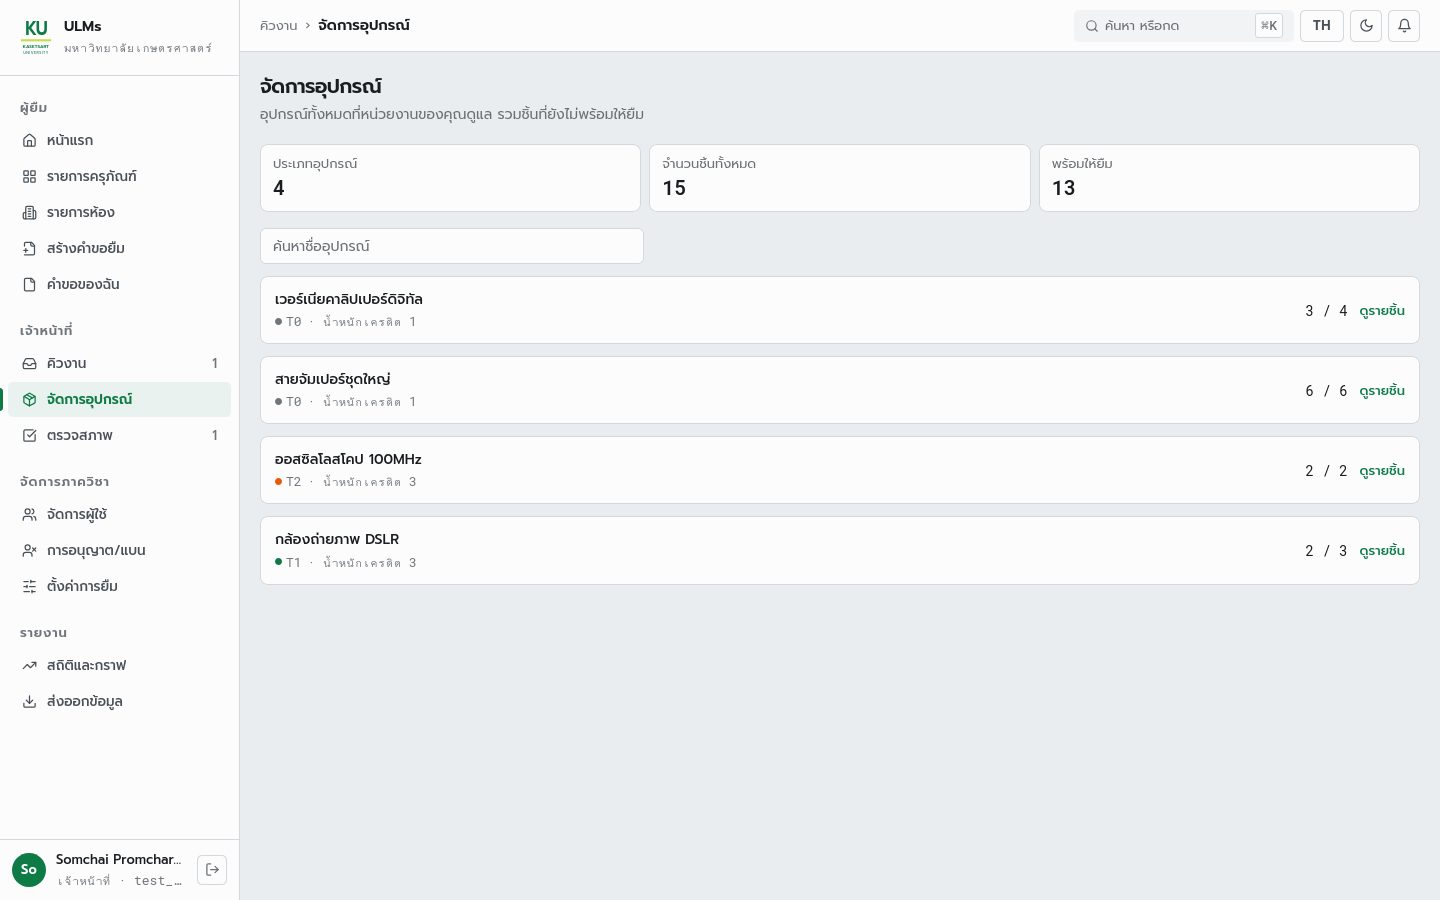
\includegraphics[width=0.92\textwidth, trim={240 300 0 60}, clip]{audit/s-inventory}
\caption{หน้า ``จัดการอุปกรณ์'' ของเจ้าหน้าที่ มีแค่รายการและปุ่มดูรายชิ้น ไม่มีปุ่มลงทะเบียนประเภท เพิ่มชิ้น หรือเพิ่มห้อง
คอมเมนต์ใน \code{inventory-page.tsx:21-23} เขียนไว้เองว่าการลงทะเบียน ``เลื่อนไปก่อน''}
\end{figure}

ฝั่ง \en{backend} มีครบแล้ว คือ \code{item.createType} \code{item.createUnit} (รับ \code{quantity} 1--200)
และ \code{item.createRoom} แต่สัญญา \en{API} ฝั่ง FE (\code{trpc-contract.ts:161-167}) ยังประกาศชื่อเก่า
\code{item.create} กับ \code{item.update} ซึ่งไม่มีอยู่จริง จึงต่อหน้าจอเข้ากับของจริงตรง ๆ ไม่ได้จนกว่าจะแก้สัญญาก่อน (F14)

\subsection{ของที่ลงทะเบียนเสร็จแล้ว ทำไมยังไม่มีใครยืมได้}

สถานการณ์ S5 และ S1 ลงทะเบียนของผ่าน \en{API} แล้วให้บัญชีผู้ยืมส่งคำขอทันที ผลคือถูกปฏิเสธทุกบรรทัด

\begin{lstlisting}
loan.create -> 200  rejected: [{ code: "NOT_ELIGIBLE",
                                 detail: { reason: "NO_RULES_CONFIGURED" } }]
\end{lstlisting}

สาเหตุอยู่ที่ \code{eligibility.service.ts:94} ของแต่ละชิ้นต้องมีแถวใน \code{Eligibility} ที่จับคู่
(หน่วยงาน, บทบาท) ไว้ก่อน ของที่ \en{seed} ยืมได้เพราะสคริปต์ \en{seed} เขียนแถวให้เอง
ของที่เจ้าหน้าที่ลงทะเบียนใหม่จึงต้องเรียกขั้นที่สาม \code{item.setEligibility} เสมอ

\begin{figure}[H]
\centering
\begin{tikzpicture}[node distance=5mm]
  \node[blk, text width=3.3cm, fill=rstf!8, draw=rstf!45] (t) {\code{item.createType}\\[1pt]\scriptsize\color{muted}ชื่อ น้ำหนักเครดิต รูป};
  \node[blk, text width=3.3cm, fill=rstf!8, draw=rstf!45, right=of t] (u) {\code{item.createUnit}\\[1pt]\scriptsize\color{muted}tier หน่วยงาน จำนวน};
  \node[blk, text width=3.3cm, fill=flag!10, draw=flag, line width=1pt, right=of u] (e) {\code{item.setEligibility}\\[1pt]\scriptsize\color{muted}ใครยืมได้บ้าง};
  \node[blk, text width=2.6cm, fill=rbor!8, draw=rbor!45, right=of e] (b) {ผู้ยืมส่งคำขอได้};
  \draw[ar] (t)--(u); \draw[ar] (u)--(e); \draw[ar] (e)--(b);
  \node[lbl, below=1.5mm of e, text width=3.8cm, text=flag] {ขาดขั้นนี้ = \code{NOT\_ELIGIBLE}\\ไม่มีข้อความเตือนตอนลงทะเบียน};
\end{tikzpicture}
\caption{การลงทะเบียนอุปกรณ์หนึ่งชนิดจริง ๆ คือสามคำสั่ง หน้าจอลงทะเบียนที่จะทำต้องรวมทั้งสามขั้นในฟอร์มเดียว}
\end{figure}

\subsection{เพิ่มจำนวนชิ้นให้ของที่มีอยู่แล้ว ทำได้จริงหรือ}

ตัวอย่าง ``ได้ Arduino เพิ่มอีก 10 ชิ้น'' ทดสอบใน S5 ด้วยการเรียก \code{createUnit} ครั้งที่สองกับประเภทเดิม ผลเสียทั้งสองแบบ

\begin{table}[H]
\centering\small
\begin{tabular}{L{4.6cm}L{4.4cm}L{5.4cm}}
\toprule
\sansall\bfseries ลำดับที่ทำ & \sansall\bfseries ผล & \sansall\bfseries สาเหตุ \\
\midrule
T0 ลงทะเบียน 2 ชิ้น แล้วเพิ่มอีก 3 ชิ้น & \textcolor{bad}{409 \code{SERIAL\_ALREADY\_IN\_USE}} & เลขที่ระบบสร้างให้เริ่มนับ \code{-1} ใหม่ทุกครั้ง ชนกับชุดแรก \\
T1 ลงทะเบียน 2 ชิ้น ตั้งสิทธิ์ แล้วเพิ่มอีก 3 ชิ้น (ใส่เลขชุดใหม่) & เพิ่มสำเร็จ แต่ยืมชิ้นใหม่ได้ \textcolor{bad}{\code{NOT\_ELIGIBLE}} & \code{setEligibility} เขียนสิทธิ์ให้เฉพาะชิ้นที่มีอยู่ตอนเรียก ชิ้นที่เพิ่มทีหลังไม่ได้ตาม \\
\bottomrule
\end{tabular}
\caption{ผลรันจริงจาก \code{results/s5\_registration.json}}
\end{table}

\begin{lstlisting}
// backend/src/item/item.management.service.ts:898-909 (buildSerials, shortened)
const base = input.serialNo ?? `${itemName...}-${input.itemKey}`;   // same base every call
if (input.quantity === 1) return [input.serialNo ?? `${base}-1`];
return Array.from({ length: input.quantity }, (_, index) => `${base}-${index + 1}`);
\end{lstlisting}

\subsection{T1 ต้องติด serial ทุกชิ้นจริงหรือ}

ตอนนี้ \en{backend} บังคับ ส่ง T1 โดยไม่มี serial จะได้
\code{400 SERIAL\_REQUIRED\_FOR\_TIER} จากฟังก์ชัน \code{buildSerials}
(\code{item.management.service.ts} บรรทัด 881--887) คอมเมนต์ในโค้ดอ้างข้อเสนอโครงการ §5.4 ที่เขียนว่า serial ติดบน T1--T2
ซึ่งตรงกับ SRS FR-EQP-06 และ FR-PKP-01 แต่ขัดกับข้อตัดสินของทีมที่ให้ T1 ไม่ติด serial

\fstep{คำตัดสิน}
F06 \vok{} ข้อคิดเห็นถูก FR-EQP-01/03/04 ระดับสูงยังไม่มีหน้าจอ \quad
F24 \vbad{} เพิ่มจำนวนชิ้นซึ่งเป็นสิ่งที่ dev ขอโดยตรง ทำไม่ได้ทั้ง T0 และ T1

\fstep{ข้อเสนอ}
\begin{itemize}
\item \textbf{FE} หน้า ``ลงทะเบียนอุปกรณ์'' ฟอร์มเดียวครบสามขั้น และปุ่ม ``เพิ่มจำนวน'' ในแถวของประเภทเดิม
      ต้องแก้ \code{trpc-contract.ts} ให้มี \code{createType} \code{createUnit} \code{createRoom} \code{setEligibility} ก่อน
\item \textbf{BE} \code{createUnit} นับเลขต่อจากเลขสูงสุดที่มีอยู่ และคัดลอกสิทธิ์ของประเภทเดิมให้ชิ้นใหม่
      (หรือเก็บสิทธิ์ระดับประเภทแทนระดับชิ้น ซึ่งเป็นการเปลี่ยนตาราง ต้องผ่าน BE-lead)
\item \textbf{BE} ตาม ข้อตัดสิน T1 ไม่บังคับ serial ใช้เลขที่ระบบสร้างแบบเดียวกับ T0
\item \textbf{SA} แก้ FR-EQP-03 (ตัด ``ผูก Serial ตอน allocation'') FR-EQP-06 (เหลือ T2) FR-PKP-01 (ตัด T1) --- ภาคผนวก ง
\end{itemize}

% -----------------------------------------------------------------------------
\section{ตัวเลข ``ว่าง 3 ชิ้น'' นับจากอะไร}
\label{sec:counter}
% -----------------------------------------------------------------------------
\fmeta{F04}{dev ข้อ 4 ``เลขจำนวนของที่ Available backend นับผิด ตอนนี้นับตอนเตรียมของ อยากให้นับตอนอนุมัติ''}{BE · SA}

\subsection{สองหน้าจอ เวลาเดียวกัน ตัวเลขไม่เท่ากัน}

\fstep{ตัวอย่าง}
กล้อง DSLR มี 3 ตัว นิสิตคนหนึ่งขอยืมและเจ้าหน้าที่จัดเตรียมไว้แล้ว 1 ตัว ภาพสองภาพข้างล่างถ่ายห่างกันไม่ถึงนาที (15 ก.ย. 12:58)

\begin{figure}[H]
\centering
\begin{minipage}[t]{0.40\textwidth}\centering
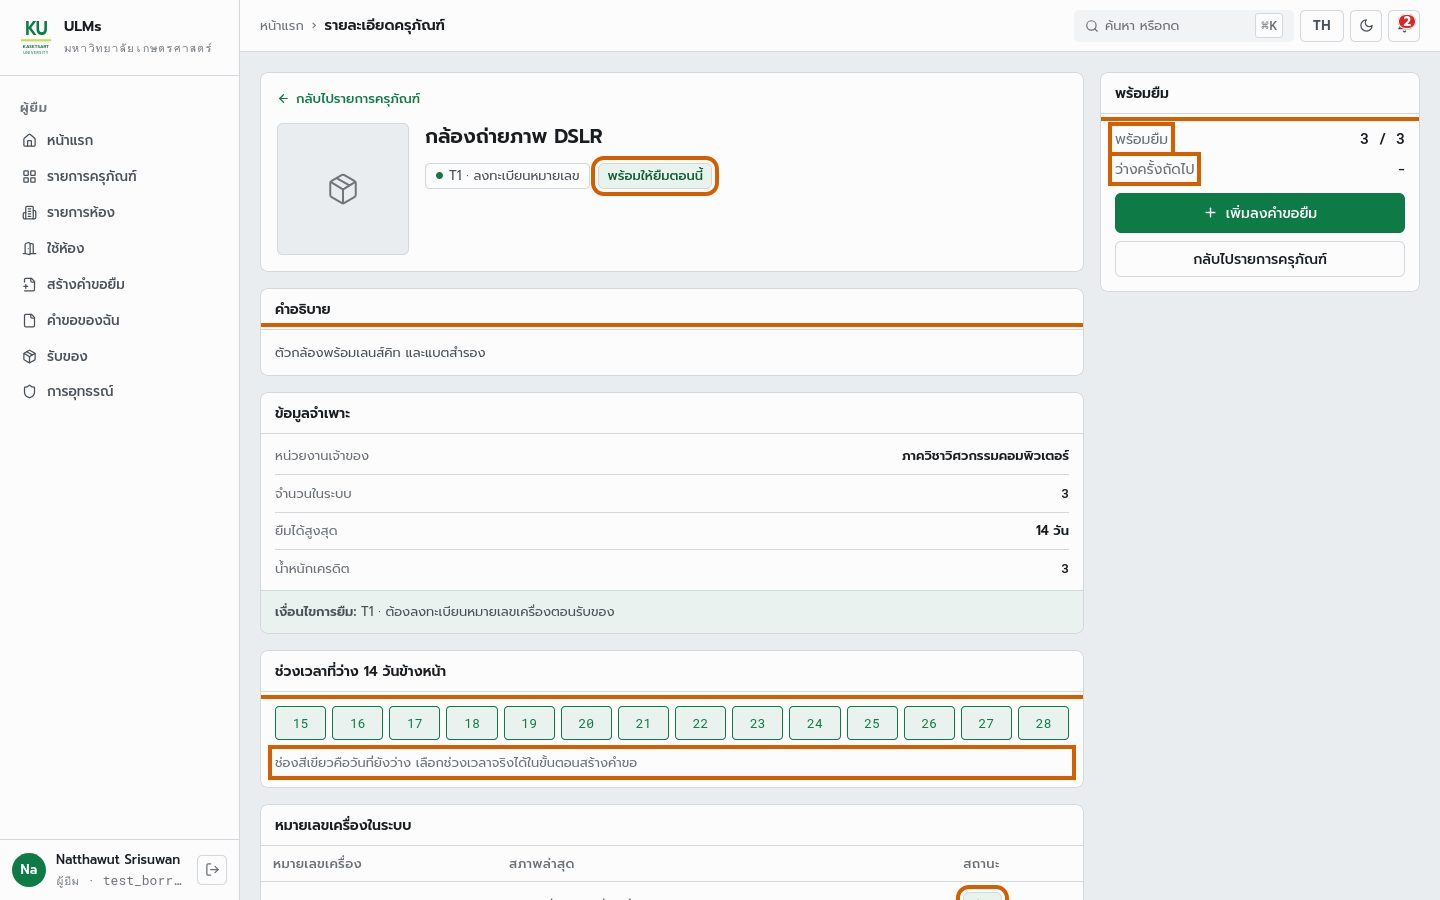
\includegraphics[width=\linewidth, trim={1100 610 20 72}, clip]{audit/b-detail-t1}\\[2pt]
{\sansall\scriptsize \rbor{} หน้ารายละเอียด: \textbf{3 / 3}}
\end{minipage}\hfill
\begin{minipage}[t]{0.57\textwidth}\centering
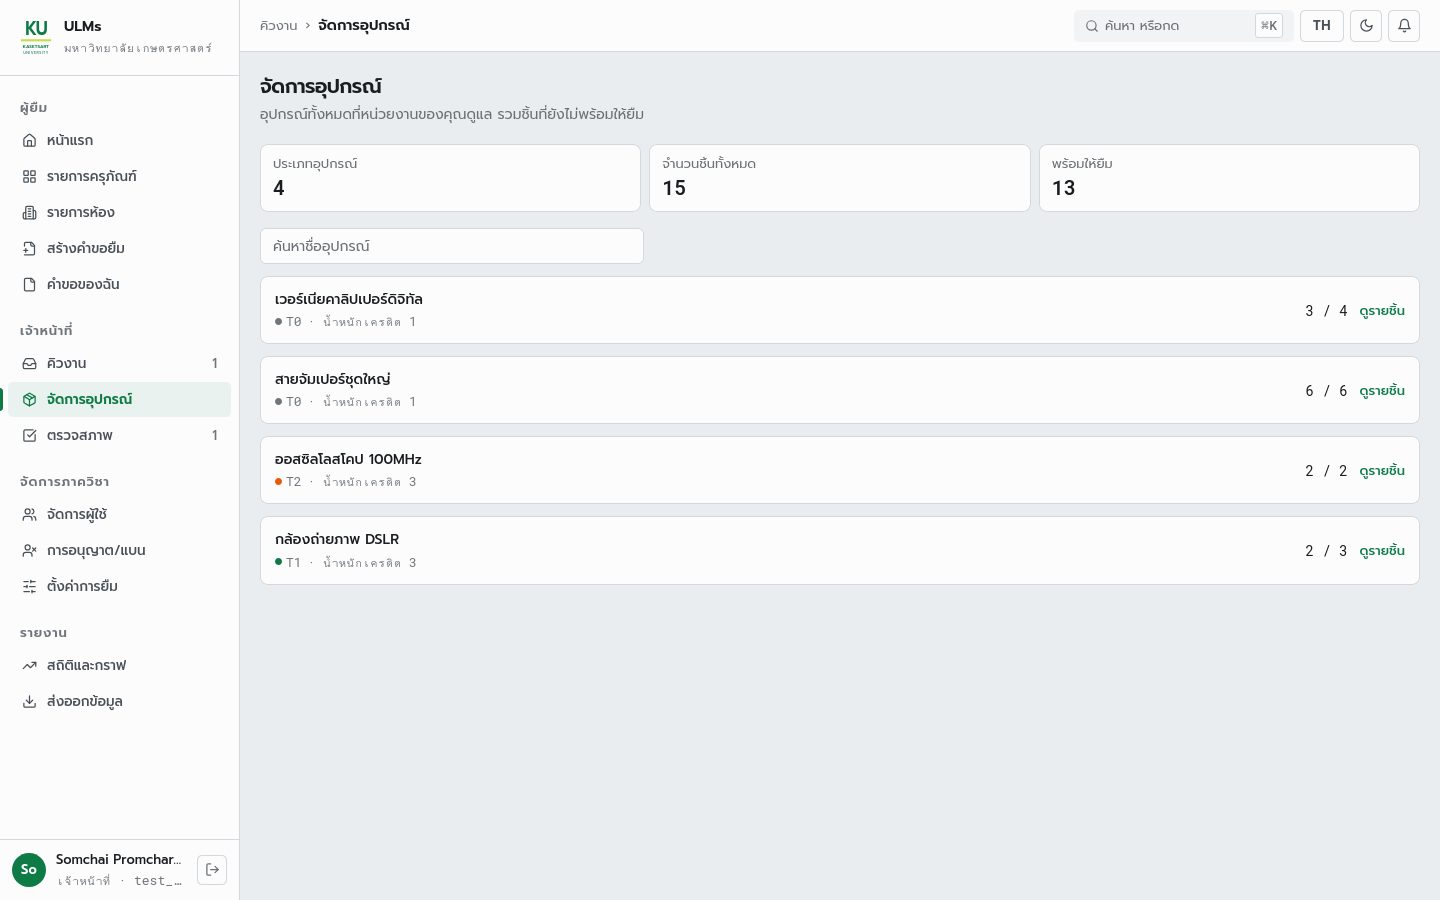
\includegraphics[width=\linewidth, trim={260 310 20 140}, clip]{audit/s-inventory}\\[2pt]
{\sansall\scriptsize \rstf{} หน้าจัดการอุปกรณ์: \textbf{2 / 3}}
\end{minipage}
\caption{ของชิ้นเดียวกัน เวลาเดียวกัน ผู้ยืมเห็นว่าว่างครบ เจ้าหน้าที่เห็นว่าว่าง 2}
\end{figure}

\fstep{แผนว่าไว้}
แผนเองตอบไม่ตรงกันสามแบบ ว่าของถูก ``กันไว้'' เมื่อไร
\begin{itemize}
\item \textbf{ตอนส่งคำขอ} --- SDS กรณีใช้งานส่งคำขอ ผลลัพธ์คือ \emph{``มีแถวใน Reservations สถานะ Pending หรือ Approved และของถูกกันไว้แล้ว''}
\item \textbf{ตอนอนุมัติ} --- FR-APV-05 \emph{``เมื่อคำขอได้รับการอนุมัติ ระบบต้องสร้าง Allocation''} (ตรงกับที่ dev ขอ)
\item \textbf{ตอนจัดเตรียม} --- ข้อเสนอโครงการ ตารางงานประจำวัน \emph{``อุปกรณ์ถูกกันไว้ (reserved) และนัดวันรับ''}
\end{itemize}
และ FR-BRW-03 / FR-EQP-07 ต้องการ ``จำนวนคงเหลือ'' กับ ``วันที่พร้อมให้ยืม'' แบบเรียลไทม์

\subsection{เดินตามการยืมหนึ่งครั้ง ตัวนับแต่ละชุดขยับตอนไหน}

\fstep{ระบบทำจริง}
สถานการณ์ S1 ลงทะเบียน T1 สามชิ้น แล้วเดินคำขอหนึ่งใบผ่านทุกสถานะ หลังแต่ละขั้นอ่านตัวนับทั้งสามที่ \en{API} มี

\begin{table}[H]
\centering\small
\begin{tabular}{L{5.2cm}ccc}
\toprule
\sansall\bfseries หลังขั้นนี้ &
\sansall\bfseries \code{item.getAvailability} &
\sansall\bfseries \code{item.list} &
\sansall\bfseries \code{item.listManaged} \\
& \scriptsize\rbor{} รายละเอียด & \scriptsize\rbor{} รายการครุภัณฑ์ & \scriptsize\rstf{} จัดการอุปกรณ์ \\
\midrule
0 ลงทะเบียน 3 ชิ้น & 3 & 3 & 3 \\
0b มีคำขอของสัปดาห์หน้า 1 ใบ & 3 & 3 & 3 \\
1 ส่งคำขอวันนี้ (T1 อนุมัติอัตโนมัติ) & 3 & 3 & 3 \\
2 อนุมัติแล้ว & 3 & 3 & 3 \\
3 เจ้าหน้าที่จัดเตรียม & 3 & 3 & \textbf{\textcolor{rstf}{2}} \\
4 ส่งมอบ & \textbf{\textcolor{rbor}{2}} & \textbf{\textcolor{rbor}{2}} & 2 \\
5 รับคืน (ยังไม่ตรวจสภาพ) & \textbf{\textcolor{bad}{3}} & \textbf{\textcolor{bad}{3}} & 2 \\
6 ตรวจสภาพแล้ว & 3 & 3 & 3 \\
\bottomrule
\end{tabular}
\caption{ผลรันจริงจาก \code{results/s1\_counters.json} สองคอลัมน์แรกให้ค่าเดียวกันเสมอเพราะใช้ฟังก์ชันเดียวกัน}
\label{tab:s1}
\end{table}

\begin{figure}[H]
\centering
\begin{tikzpicture}[x=1.95cm, y=0.62cm]
  \foreach \y in {0,1,2,3} { \draw[rule, line width=0.3pt] (0,\y) -- (6.4,\y); \node[lbl, anchor=east] at (-0.05,\y) {\y}; }
  \foreach \x/\t in {0/ลงทะเบียน,1/ส่งคำขอ,2/อนุมัติ,3/จัดเตรียม,4/ส่งมอบ,5/รับคืน,6/ตรวจแล้ว}
    { \node[lbl, anchor=north, text width=1.7cm] at (\x+0.2,-0.2) {\t}; }
  % proposed: held from the request until inspection
  \draw[ctr, line width=1.3pt, dashed] (0,3.12) -- (1,3.12) -- (1,2.12) -- (6,2.12) -- (6,3.12) -- (6.4,3.12);
  % staff
  \draw[rstf, line width=1.6pt] (0,2.96) -- (3,2.96) -- (3,1.96) -- (6,1.96) -- (6,2.96) -- (6.4,2.96);
  % borrower
  \draw[rbor, line width=1.6pt] (0,2.8) -- (4,2.8) -- (4,1.8) -- (5,1.8) -- (5,2.8) -- (6.4,2.8);
  \draw[rbor, line width=1.6pt] (0.2,-1.75) -- ++(0.35,0) node[tag, text=rbor, anchor=west] {\;ผู้ยืมเห็น};
  \draw[rstf, line width=1.6pt] (2.0,-1.75) -- ++(0.35,0) node[tag, text=rstf, anchor=west] {\;เจ้าหน้าที่เห็น};
  \draw[ctr, line width=1.3pt, dashed] (4.0,-1.75) -- ++(0.35,0) node[tag, text=ctr, anchor=west] {\;ข้อเสนอ};
  \draw[flag, line width=0.8pt, rounded corners=2pt] (4.85,1.55) rectangle (5.15,3.0);
  \node[lbl, text=flag, anchor=west] at (5.2,3.6) {ของยังไม่ผ่านตรวจ แต่ขึ้นว่างแล้ว};
\end{tikzpicture}
\caption{จำนวนชิ้นที่ว่างตามขั้นของการยืม (ตารางที่~\ref{tab:s1}) เส้นประคือข้อเสนอ: ของถูกกันตั้งแต่ส่งคำขอจนตรวจสภาพเสร็จ}
\end{figure}

สองชุดตัวนับใช้คนละกฎ

\begin{lstlisting}
// backend/src/common/mappers/item.mapper.ts:114  -- borrower screens
export function isUnitAvailable(unit: AvailabilityUnitRow): boolean {
  return unit.Resource.ResourceStatus === 'InStorage' && unit.Resource.AllowBorrow;
}

// backend/src/item/item.management.service.ts:997  -- staff screens
private isAvailable(unit: UnitRow): boolean {
  return unit.Resource.ResourceStatus === 'InStorage' &&
         unit.Resource.AllowBorrow &&
         unit.Resource.UsageLogs.length === 0;  // no log in Pending|Prepared|Lended|Returned
}
\end{lstlisting}

\code{ResourceStatus} เปลี่ยนเป็น \code{Lended} ตอนส่งมอบ (\code{loan.service.ts:432}) และกลับเป็น \code{InStorage}
ตอนรับคืน (\code{loan.service.ts:515}) ตัวนับฝั่งผู้ยืมจึงลดตอนส่งมอบและเพิ่มกลับก่อนตรวจสภาพ
ส่วนฝั่งเจ้าหน้าที่ดู \code{UsageLog} จึงลดตั้งแต่จัดเตรียมจนตรวจเสร็จ
คำขอที่อนุมัติแล้วไม่มี \code{UsageLog} \textbf{จึงไม่ลดตัวนับชุดใดเลย}

\subsection{ทำไม dev เห็นว่า ``นับตอนเตรียมของ'' และทำไมยังไม่ครบ}

dev ดูหน้าเจ้าหน้าที่ ซึ่งลดตอนจัดเตรียมจริง แต่ผู้ยืมไม่ได้เห็นตัวเลขนั้น ผู้ยืมเห็นตัวเลขที่ลดช้ากว่าอีกขั้น
และมีจุดผิดที่หนักกว่า คือขึ้นว่างทันทีที่รับคืน ทั้งที่ของยังไม่ผ่านตรวจสภาพและอาจเสียหาย

\begin{warnbox}[title={กับดัก --- ย้ายจุดนับไปตอนอนุมัติ ตัวเลขก็ยังผิด}]
ตัวนับทั้งสองชุดตอบคำถาม ``ตอนนี้บนชั้นมีกี่ชิ้น'' แต่ผู้ยืมถามว่า ``\textbf{ช่วงวันที่ฉันจะยืม} มีกี่ชิ้น''
คำขอของสัปดาห์หน้า (แถว 0b) ไม่ควรลดตัวเลขวันนี้ แต่ต้องลดตัวเลขของสัปดาห์หน้า
ขณะที่การกันจองจริงใน \en{backend} (\code{booking-window.ts:12} \code{HOLDING\_APPROVE\_STATES = ['Pending','Approved']})
\textbf{กันตั้งแต่คำขอยังรออนุมัติ} (พิสูจน์ในหัวข้อ~\ref{sec:overlap}) ถ้าตัวเลขลดตอนอนุมัติ
ผู้ยืมคนที่สองจะเห็นว่าว่าง กดส่ง แล้วโดนปฏิเสธ \code{WINDOW\_NOT\_AVAILABLE}
\end{warnbox}

\subsection{ควรนับที่จุดไหน}

\fstep{คำตัดสิน}
\vpart{} ข้อคิดเห็นถูกว่านับผิด แต่ผิดมากกว่าที่เห็น และ ``นับตอนอนุมัติ'' ไม่ใช่ทางแก้

\fstep{ข้อเสนอ}
\begin{itemize}
\item \textbf{BE} รวมเป็นฟังก์ชันเดียว \emph{ว่างในช่วง [เริ่ม, คืน]} = ชิ้นที่ยืมได้ ลบชิ้นที่มีคำขอ \code{Pending/Approved} ซ้อนช่วง
      (รวม \code{BufferTime}) ลบชิ้นที่มี \code{UsageLog} ยังไม่ \code{Inspected} ใช้ตัวกรองเดียวกับ \code{clashingWindowFilter}
      ทุกหน้าจอเรียกฟังก์ชันนี้ ตัวนับ ``ตอนนี้'' คือช่วง [วันนี้, วันนี้]
\item \textbf{SA} ตัดสินจุดกันของเป็น ``ตั้งแต่ส่งคำขอ'' ให้ตรงกับ \en{backend} ที่ทำงานอยู่ แล้วแก้ FR-APV-05 และข้อความในข้อเสนอให้ตรงกัน
\item ฟังก์ชันนี้คือข้อมูลชุดเดียวกับที่ปฏิทินในหัวข้อถัดไปต้องใช้ ทำครั้งเดียวได้สองข้อ
\end{itemize}

% -----------------------------------------------------------------------------
\section{ผู้ยืมเลือกวันยืมจากข้อมูลอะไร}
\label{sec:calendar}
% -----------------------------------------------------------------------------
\fmeta{F01 · F09}{dev ข้อ 1 ``เวลาว่างของ เปลี่ยนเป็นแบบปฏิทิน มีช่องกดได้กดไม่ได้'' · ตรวจเจอเพิ่ม}{BE · FE · SA}

\fstep{ตัวอย่าง}
นาย ก ต้องการกล้อง DSLR วันที่ 16--18 ก.ย. แต่วันที่ 17 ทั้ง 3 ตัวถูกจองโดยคนอื่นแล้ว
นาย ก ควรรู้ตั้งแต่ตอนเลือกวัน ไม่ใช่รู้ตอนกดส่งแล้วโดนปฏิเสธ

\fstep{แผนว่าไว้}
FR-REQ-02 บังคับวันรับและวันคืน 1--14 วัน FR-EQP-07 ให้แสดงวันที่พร้อมให้ยืม ข้อเสนอโครงการขอบเขต R01 มี
``จองล่วงหน้าแบบเลือกช่วงเวลา พร้อมปฏิทิน'' และข้อตัดสินของทีมกำหนดเป็นปฏิทินแบบช่วงวันที่มีวันเทา

\subsection{หน้าสร้างคำขอตอนนี้ตรวจของว่างกับวันไหน}

\fstep{ระบบทำจริง}
\begin{figure}[H]
\centering
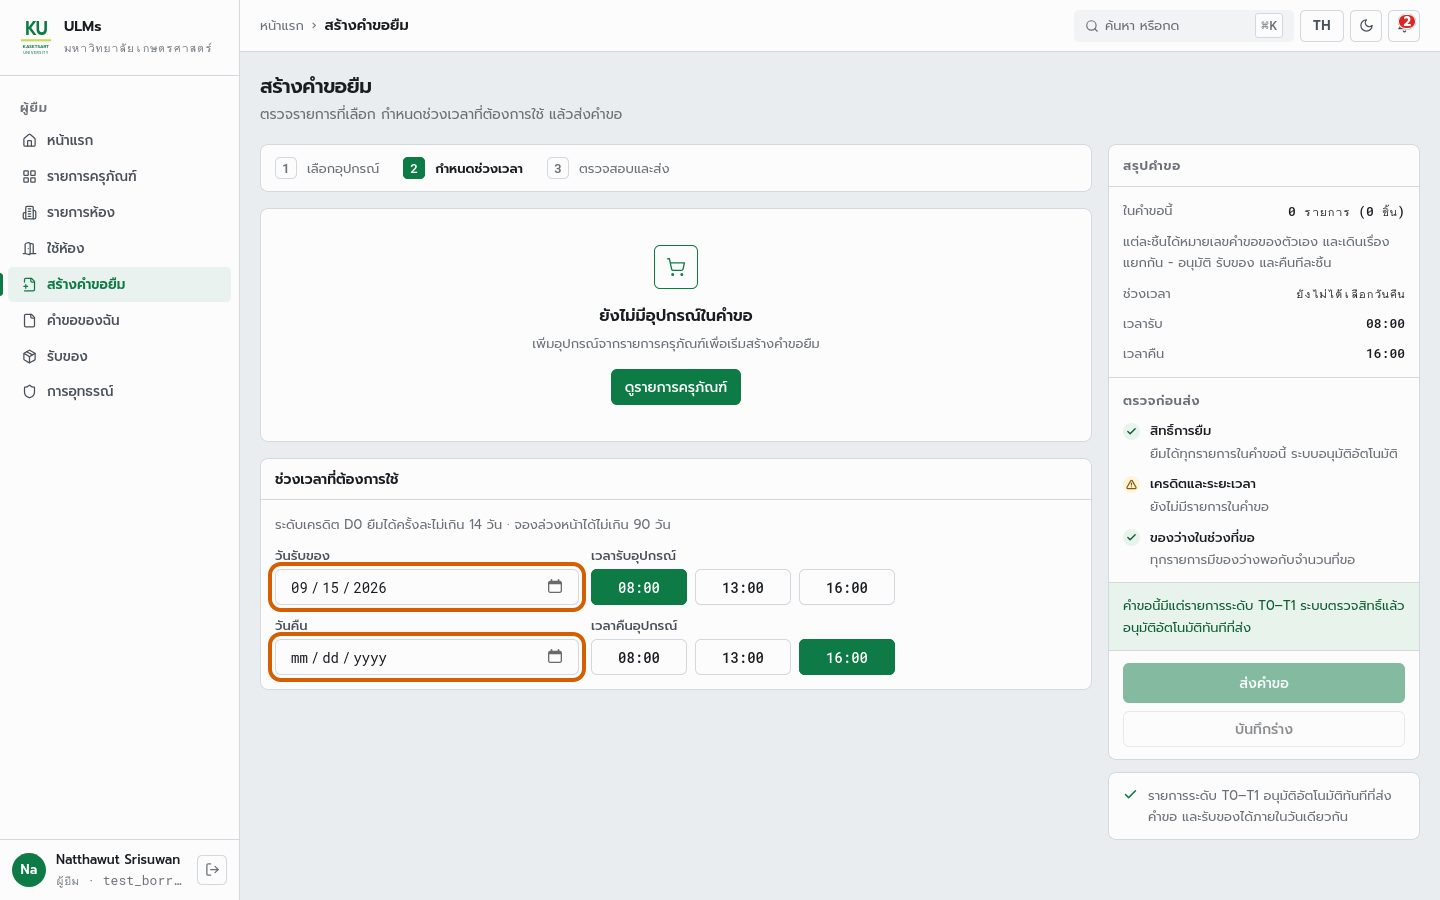
\includegraphics[width=0.95\textwidth, trim={240 200 0 50}, clip]{audit/b-request}
\caption{หน้าสร้างคำขอ วันรับ/วันคืนเป็นช่องกรอกวันที่ธรรมดาสองช่อง กับปุ่มเวลา 08:00 13:00 16:00 ไม่มีข้อมูลว่าวันไหนของเต็ม}
\end{figure}

ป้าย ``ของว่างในช่วงที่ขอ'' ทางขวามือไม่ได้ตรวจช่วงที่ขอจริง

\begin{lstlisting}
// frontend/src/features/borrower/request/request-page.tsx:124
const short = rows.filter((r) => r.qty > r.item.availableUnits);  // count for "now", not the picked dates
\end{lstlisting}

\subsection{แถบ 14 วันสีเขียวบอกอะไรจริง}

\begin{figure}[H]
\centering
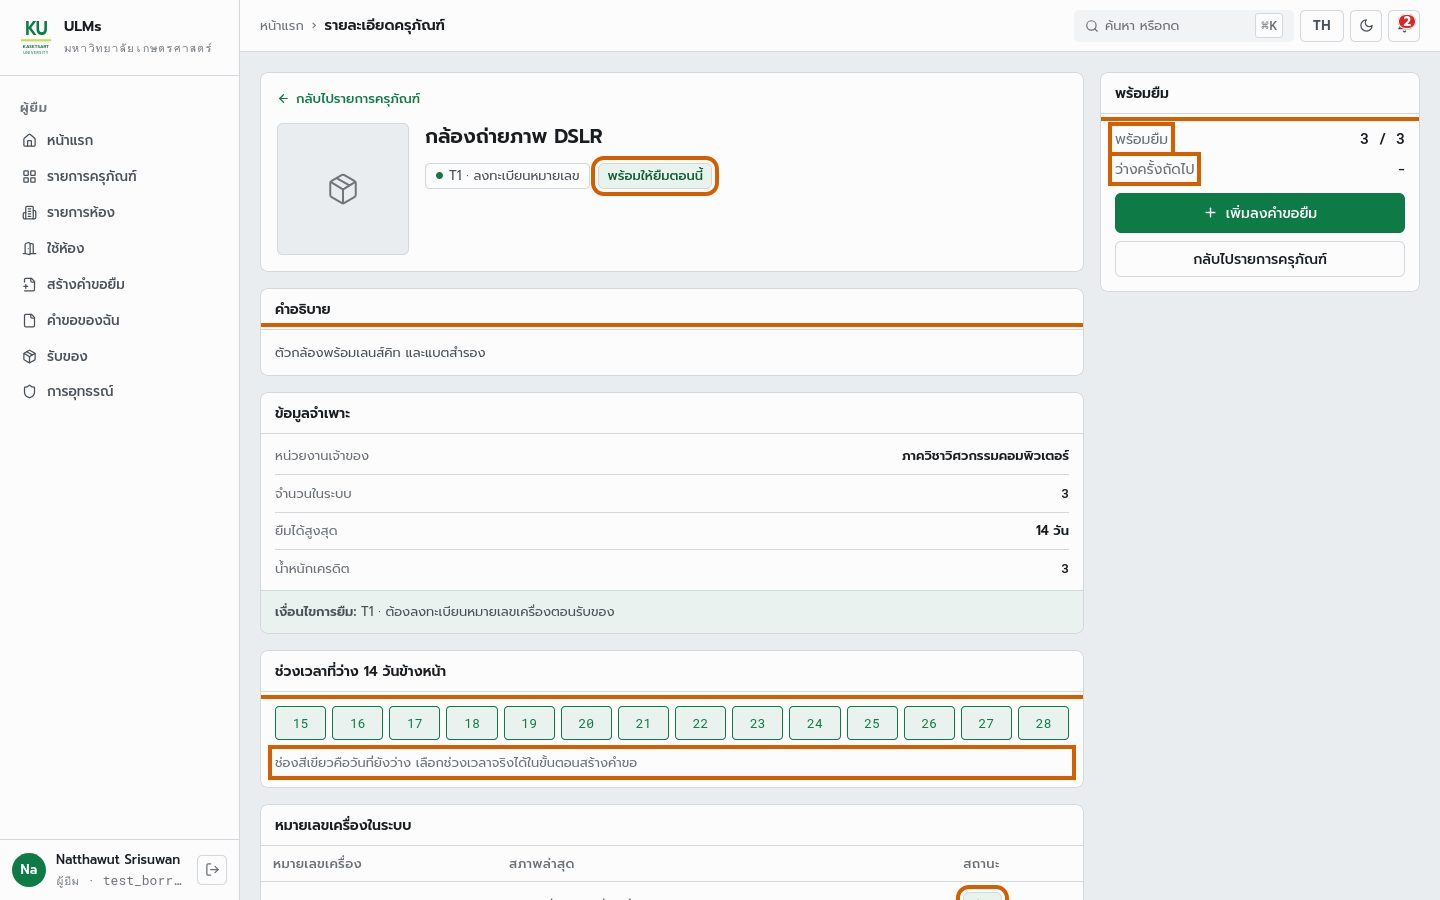
\includegraphics[width=0.9\textwidth, trim={260 110 355 650}, clip]{audit/b-detail-t1}
\caption{แถบ ``ช่วงเวลาที่ว่าง 14 วันข้างหน้า'' ในหน้ารายละเอียด เขียวทั้งแถบ}
\end{figure}

แถบนี้สร้างจากตัวนับ ``ตอนนี้'' กับ \code{nextAvailableAt} เท่านั้น (\code{equipment-detail-page.tsx:94} \code{buildDays(availableUnits, nextAvailableAt)})
เพราะ \en{backend} ไม่มีข้อมูลรายวันให้ ในแถว 0b ของตารางที่~\ref{tab:s1} มีคำขอของสัปดาห์หน้าอยู่แล้ว ตัวนับยังเป็น 3
แถบจึงเขียวทุกวัน\textbf{แม้วันนั้นจะถูกจองเต็ม} ผู้ยืมอ่านแถบนี้เป็นปฏิทินและเชื่อมัน ซึ่งอันตรายกว่าไม่มีแถบเลย

\subsection{ปฏิทินช่วงวันที่ตกลงกัน ควรทำงานอย่างไร}

\fstep{คำตัดสิน}
F01 \vdec[ถูก ตัดสินแล้ว] \quad F09 \vbad{} ข้อมูลที่หน้าจอใช้ตัดสินว่าของพอเป็นคนละช่วงเวลากับที่ผู้ยืมเลือก

\fstep{ข้อเสนอ}
\begin{figure}[H]
\centering
\begin{tikzpicture}[x=1.05cm, y=0.78cm]
  \node[tag, anchor=west] at (-0.5,1.1) {กันยายน 2569 \quad \color{muted}\normalfont\scriptsize กล้อง DSLR · ขอ 1 ตัว · แถบเครดิต D0 ยืมได้ไม่เกิน 14 วัน};
  \foreach \d/\n in {0/จ,1/อ,2/พ,3/พฤ,4/ศ,5/ส,6/อา} \node[lbl] at (\d,0.35) {\n};
  % Sep 2026 starts on Tuesday (column 1). Days before today (15) are past.
  \foreach \day in {1,...,30} {
    \pgfmathtruncatemacro{\idx}{\day}
    \pgfmathtruncatemacro{\col}{mod(\day,7)}
    \pgfmathtruncatemacro{\row}{(\day)/7}
    \pgfmathtruncatemacro{\colfix}{\col}
    \coordinate (c\day) at (\col,-\row);
  }
  \foreach \day in {1,...,30} {
    \pgfmathtruncatemacro{\col}{mod(\day,7)}
    \pgfmathtruncatemacro{\row}{\day/7}
    \ifnum\day<15
      \node[draw=rule, fill=rule!40, text=muted, minimum width=0.92cm, minimum height=0.66cm, font=\sansall\scriptsize] at (\col,-\row) {\day};
    \else\ifnum\day=17
      \node[draw=rule, fill=rule!70, text=muted, minimum width=0.92cm, minimum height=0.66cm, font=\sansall\scriptsize] at (\col,-\row) {\day};
    \else\ifnum\day<30
      \ifnum\day>18
        \node[draw=rbor!50, fill=white, minimum width=0.92cm, minimum height=0.66cm, font=\sansall\scriptsize] at (\col,-\row) {\day};
      \else
        \node[draw=rbor!50, fill=white, minimum width=0.92cm, minimum height=0.66cm, font=\sansall\scriptsize] at (\col,-\row) {\day};
      \fi
    \else
      \node[draw=rbor!50, fill=white, minimum width=0.92cm, minimum height=0.66cm, font=\sansall\scriptsize] at (\col,-\row) {\day};
    \fi\fi\fi
  }
  % selected range 19-23 (Sat .. Wed)
  \foreach \day in {19,20,21,22,23} {
    \pgfmathtruncatemacro{\col}{mod(\day,7)}
    \pgfmathtruncatemacro{\row}{\day/7}
    \node[draw=rbor, fill=rbor!25, minimum width=0.92cm, minimum height=0.66cm, font=\sansall\scriptsize\bfseries] at (\col,-\row) {\day};
  }
  \node[lbl, anchor=west, text width=5.8cm, align=left] at (7.2,-0.4)
    {\textcolor{muted}{\rule{7pt}{7pt}} อดีต กดไม่ได้\\[2pt]
     \textcolor{rule!160}{\rule{7pt}{7pt}} 17 ก.ย. ว่าง 0 ตัว กดไม่ได้\\
     \hspace*{9pt}และ\textbf{เลือกช่วงคร่อมวันนี้ไม่ได้}\\[2pt]
     \textcolor{rbor!60}{\rule{7pt}{7pt}} ช่วงที่เลือก 19--23 ก.ย. (5 วัน)\\[2pt]
     \textcolor{muted}{เลือกวันแรกแล้ว วันที่เกิน 14 วันจากวันแรกเป็นสีเทาทันที}};
\end{tikzpicture}
\caption{ภาพปฏิทินที่เสนอ วันเทามาจากฟังก์ชัน ``ว่างในช่วง'' ในหัวข้อ~\ref{sec:counter} คำนวณแยกทีละวัน}
\end{figure}

\begin{itemize}
\item \textbf{BE} \en{query} ใหม่ เช่น \code{item.availabilityCalendar(\{ itemKey, from, to, quantity \})} คืนจำนวนว่างรายวัน
      ใช้ฟังก์ชันเดียวกับข้อ F04 ห้ามคำนวณแยกอีกชุด
\item \textbf{FE} วันที่ว่างน้อยกว่าจำนวนที่ขอเป็นสีเทา ช่วงที่เลือกคร่อมวันเทาไม่ได้ ความยาวสูงสุดตามแถบเครดิต
      ตะกร้าหลายรายการ ใช้วันที่ว่างพร้อมกันทุกรายการ (ตัดกัน) ปุ่มเวลาเดิมคงไว้
\item \textbf{FE} ป้าย ``ของว่างในช่วงที่ขอ'' ใช้ผลของช่วงที่เลือก ไม่ใช่ \code{availableUnits}
\item \textbf{SA} เพิ่ม FR ในหมวด BRW สำหรับปฏิทินอุปกรณ์ (ตอนนี้ FR-BRW-05 มีปฏิทินแค่ของ T3)
\end{itemize}

\clearpage
% =============================================================================
\part{ส่งคำขอและอนุมัติ}
% =============================================================================

\textbf{คำถามที่ภาคนี้ตอบ: คำขอที่ผู้ยืมกดส่งไปถึงระบบจริงไหม ระบบกันการจองชนกันได้ไหม และคนที่อนุมัติคือคนที่แผนกำหนดหรือไม่}

% -----------------------------------------------------------------------------
\section{กดส่งคำขอแล้ว คำขอไปอยู่ที่ไหน}
\label{sec:submit}
% -----------------------------------------------------------------------------
\fmeta{F07}{ตรวจเจอเพิ่ม (พบครั้งแรก 11 ก.ย. ยังไม่แก้)}{FE}

\fstep{ตัวอย่าง}
ผู้ยืมเลือกของ เลือกวัน กด ``ส่งคำขอ'' หน้าจอบอกสำเร็จและคำขอขึ้นใน ``คำขอของฉัน''
เจ้าหน้าที่เปิดคิวงานไม่เห็นอะไร ผู้ยืมกดรีเฟรชหน้า คำขอหายไป

\fstep{แผนว่าไว้}
FR-REQ-01 ถึง FR-REQ-10 ทั้งหมดสมมติว่าคำขอเข้าไปอยู่ในระบบ และ \en{backend} มี \code{loan.create} พร้อมใช้แล้ว

\fstep{ระบบทำจริง}
ปุ่มฝั่งผู้ยืม 8 จุดเขียนผลลงที่เก็บข้อมูลในหน่วยความจำของเบราว์เซอร์ (\code{useSubmittedRequests}) แทนการเรียก \en{API}
ห้าจุดมี \en{procedure} รอใช้อยู่แล้ว

\begin{table}[H]
\centering\small
\begin{tabular}{L{3.3cm}L{6.1cm}L{4.9cm}}
\toprule
\sansall\bfseries ปุ่ม & \sansall\bfseries ตำแหน่ง (\code{frontend/src/features/borrower/}) & \sansall\bfseries \en{backend} มีให้เรียกแล้ว \\
\midrule
ส่งคำขอ & \code{request/request-page.tsx:176} (TODO) & \textcolor{feg!70!black}{\code{loan.create}} \\
บันทึกร่าง & \code{request/request-page.tsx:192} (TODO) & ไม่มี \\
ยกเลิกคำขอ & \code{loans/my-loans-page.tsx} ผ่าน \code{submitted-requests.store.ts} & \textcolor{feg!70!black}{\code{loan.cancel}} (มี \en{hook} แล้วแต่ไม่ถูกเรียก) \\
ยืนยันรับของ + รูป & \code{pickup/pickup-page.tsx:56} (TODO) & ไม่มี (ภาค 3) \\
ขอต่ออายุ & \code{loans/my-loans-page.tsx:368} (TODO) & \textcolor{feg!70!black}{\code{loan.requestExtension}} \\
จองห้อง & \code{rooms/room-booking-page.tsx:119} (TODO) & \textcolor{feg!70!black}{\code{loan.create}} \\
ใช้ห้อง/ถ่ายรูปห้อง & \code{rooms/room-use-page.tsx:273} (TODO) & ไม่มี \\
ส่งอุทธรณ์ & \code{loans/submitted-requests.store.ts:197} (TODO) & ไม่มี \en{router} อุทธรณ์ \\
\bottomrule
\end{tabular}
\caption{ปุ่มที่หน้าจอบอกว่าสำเร็จ แต่ข้อมูลไม่ถึงฐานข้อมูล ในสถานการณ์ทดสอบทุกข้อของเล่มนี้จึงต้องเรียก \en{API} ตรงแทนการกดปุ่ม}
\end{table}

\fstep{คำตัดสิน}
\vbad{} เป็นเหตุผลเดียวที่ใหญ่ที่สุดที่วงจรยืมยังสาธิตผ่านหน้าจอไม่ได้ ทั้งที่ \en{backend} ทำงานครบ

\fstep{ข้อเสนอ}
FE ต่อสาม \en{procedure} ที่มีครบแล้วก่อน คือ \code{loan.create}, \code{loan.cancel} และ \code{loan.requestExtension}
แล้วเลิกใช้ \code{useSubmittedRequests} ในเส้นทางของคำขอจริง ส่วนยืนยันรับของและอุทธรณ์ต้องรอ \en{backend} ตามภาค 3 และ 4

% -----------------------------------------------------------------------------
\section{ของชิ้นเดียว สองคนขอช่วงเดียวกัน}
\label{sec:overlap}
% -----------------------------------------------------------------------------
\fmeta{---}{ตรวจยืนยันกฎ FR-REQ-09 และเป็นหลักฐานของข้อ F04}{---}

\fstep{ตัวอย่างและผลรันจริง}
ของ T1 ชิ้นเดียว \rbor{} ส่งคำขอ A วันที่ +3 ถึง +5 แล้ว\rstf{} (ยืมได้ตาม FR-AUTH-04) ส่งคำขอช่วงอื่นตามมา

\begin{table}[H]
\centering\small
\begin{tabular}{L{4.0cm}L{4.9cm}L{5.4cm}}
\toprule
\sansall\bfseries คำขอ & \sansall\bfseries ผล & \sansall\bfseries อ่านว่า \\
\midrule
A วันที่ +3 ถึง +5 & อนุมัติ (T1 อัตโนมัติ) & ของชิ้นนี้ถูกกันช่วง +3 ถึง +5 \\
B ช่วงเดียวกับ A & \textcolor{bad}{\code{WINDOW\_NOT\_AVAILABLE}} & ซ้อนทั้งช่วง ปฏิเสธถูก \\
C วันที่ +5 ถึง +7 & \textcolor{bad}{\code{WINDOW\_NOT\_AVAILABLE}} & ซ้อนวันสุดท้าย ปฏิเสธถูก \\
D วันที่ +6 ถึง +8 & อนุมัติ & ติดกันแต่ไม่ซ้อน ถูก \\
E วันที่ +12 ถึง +14 & อนุมัติ & ห่างกัน ถูก \\
\bottomrule
\end{tabular}
\caption{ผลรันจริงจาก \code{results/s2\_overlap.json}}
\end{table}

\begin{goodbox}[title={ตรวจแล้ว --- \en{backend} กันการจองซ้อนถูกต้อง}]
การตรวจช่วงเวลาใช้ช่วงแบบครึ่งเปิด \code{StartTime < to AND EndTime > from} บวก \code{BufferTime} ทั้งสองข้าง
(\code{booking-window.ts:45}) และทำใน \en{transaction} ระดับ \en{Serializable} พร้อมลองใหม่ 3 ครั้ง
ตรงกับ FR-REQ-09 และตรงกับข้อตัดสินเรื่องปฏิทิน จุดที่ต้องแก้คือ\textbf{หน้าจอยังไม่ได้เอาข้อมูลนี้มาแสดง}ก่อนผู้ยืมกดส่ง
\end{goodbox}

% -----------------------------------------------------------------------------
\section{ใครอนุมัติคำขอระดับไหน}
\label{sec:approver}
% -----------------------------------------------------------------------------
\fmeta{F11}{ตรวจเจอเพิ่ม}{SA}

\fstep{แผนว่าไว้ และระบบทำจริง}

\begin{table}[H]
\centering\small
\begin{tabular}{L{1.1cm}L{4.3cm}L{3.3cm}L{5.6cm}}
\toprule
\sansall\bfseries ระดับ & \sansall\bfseries SRS & \sansall\bfseries โค้ด \scriptsize(\code{approval-policy.ts}) & \sansall\bfseries ผลรันจริง \\
\midrule
T0 & \rsys{} อัตโนมัติ (FR-REQ-04) & \rsys{} อัตโนมัติ & --- \\
T1 & \rsys{} อัตโนมัติ D0--D1 · \rsup{} D2--D3 (FR-REQ-05) & ตรงกัน & D0 ได้ \code{approved} ทันที (S1) \\
T2 & \rsup{} เสมอ (FR-REQ-06) & \rsup{} & \rstf{} กดอนุมัติได้ 403 \code{APPROVAL\_NEEDS\_SUPERVISOR} \rsup{} อนุมัติได้ (S4) \\
T3 & \textcolor{bad}{ไม่มีข้อกำหนด} & \rstf{} & ได้ \code{pending} รอเจ้าหน้าที่ (S3) \\
\bottomrule
\end{tabular}
\end{table}

\begin{warnbox}[title={ต้องตัดสิน --- T3 ใครอนุมัติ}]
ข้อเสนอโครงการเขียนว่า T3 ``อนุมัติอัตโนมัติหลังตรวจสิทธิ์'' แต่โค้ดส่งให้เจ้าหน้าที่ และหน้าจองห้อง
บอกผู้ยืมว่า ``รอเจ้าหน้าที่อนุมัติก่อนจึงจะเข้าใช้ได้'' ถ้ามองตามเกณฑ์ของอาจารย์ (ทุกบทบาทมีปฏิสัมพันธ์)
การให้เจ้าหน้าที่อนุมัติ T3 ทำให้การจองห้องมีคนสองฝ่าย จึงแนะนำให้คงตามโค้ด แล้วเพิ่ม FR ใน SRS
\end{warnbox}

\fstep{คำตัดสิน}
\vpart[ต้องตัดสิน] T0--T2 \vok[ตรงแผน]

% -----------------------------------------------------------------------------
\section{อาจารย์อนุมัติ serial A แต่เจ้าหน้าที่จัด serial B ได้หรือไม่}
\label{sec:serialab}
% -----------------------------------------------------------------------------
\fmeta{F12}{ตรวจเจอเพิ่ม}{BE}

\fstep{ตัวอย่าง}
ออสซิลโลสโคปมีสองเครื่อง A และ B นิสิตเลือกเครื่อง A (FR-REQ-07 ให้ผู้ยืมเลือก serial ของ T2)
อาจารย์อนุมัติเครื่อง A เพราะเครื่อง B มีประวัติเสีย

\fstep{ระบบทำจริง}
สถานการณ์ S4 ให้เจ้าหน้าที่เรียก \code{loan.allocate} พร้อมระบุเครื่อง B

\begin{table}[H]
\centering\small
\begin{tabular}{L{1.1cm}L{6.9cm}L{6.3cm}}
\toprule
\sansall\bfseries ผู้ทำ & \sansall\bfseries คำสั่ง & \sansall\bfseries ผล \\
\midrule
\rbor & ขอเครื่อง A & \code{pending} \\
\rsup & อนุมัติ & สำเร็จ \\
\rstf & \code{allocate} ระบุเครื่อง B & \textcolor{bad}{\textbf{สำเร็จ} \code{status=Prepared serial=S4B-...}} \\
\rstf & \code{swapUnit} สลับกลับเป็น A & 403 \code{UNIT\_SWAP\_NOT\_ALLOWED} \\
\rstf & ส่งมอบเครื่อง B & สำเร็จ \\
\bottomrule
\end{tabular}
\caption{ผลรันจริงจาก \code{results/s4\_handover.json}}
\end{table}

\begin{lstlisting}
// backend/src/loan/loan.service.ts:275  allocate -- any tier may take another unit
const target =
  input.resourceKey === undefined || input.resourceKey === reservation.Resource.ResourceKey
    ? reservation.Resource
    : await this.resolveSwapTarget(user, reservation.Resource, input.resourceKey);

// backend/src/loan/loan.service.ts:351  swapUnit -- the same move, but refused unless T1
throw new BusinessError('UNIT_SWAP_NOT_ALLOWED', { ... });
\end{lstlisting}

\begin{badbox}[title={ผิดจริง --- สองประตูทำเรื่องเดียวกันแต่ล็อกแค่ประตูเดียว}]
\code{swapUnit} ห้ามเปลี่ยนเครื่องของ T2 แต่ \code{allocate} ทำสิ่งเดียวกันได้โดยไม่ตรวจระดับ
ผลคือเครื่องที่ออกจากเคาน์เตอร์ไม่ใช่เครื่องที่อาจารย์อนุมัติ และอาจารย์ไม่มีทางรู้
\end{badbox}

\fstep{คำตัดสิน}
\vbad{}

\fstep{ข้อเสนอ}
BE ให้ \code{allocate} ปฏิเสธ \code{resourceKey} ที่ต่างจากที่อนุมัติเมื่อเป็น T2 ด้วยการตรวจเดียวกับ \code{swapUnit}
เมื่อ T1 ไม่มี serial และเปลี่ยนชิ้นนอกระบบแล้ว (ข้อตัดสิน) \code{swapUnit} จะไม่มีผู้ใช้ ทีม BE เลือกได้ว่าจะเก็บหรือลบ

\clearpage
% =============================================================================
\part{เตรียมของและส่งมอบ}
% =============================================================================

\textbf{คำถามที่ภาคนี้ตอบ: ตอนของออกจากเคาน์เตอร์ ใครเป็นคนยืนยัน และหลักฐานสภาพของตอนนั้นเป็นของใคร}

% -----------------------------------------------------------------------------
\section{ใครเป็นคนยืนยันว่าของออกจากเคาน์เตอร์แล้ว}
\label{sec:handover}
% -----------------------------------------------------------------------------
\fmeta{F05c (ส่วนแรก)}{dev ข้อ 5 ``ตอนนี้ staff กดส่งมอบแล้ว ผู้ยืมไม่ต้องส่งรูปตอนรับของ''}{BE · FE · SA}

\fstep{ตัวอย่าง}
เจ้าหน้าที่จัดเตรียมกล้อง DSLR ไว้แล้ว นิสิตมาที่เคาน์เตอร์ ในระบบตอนนี้มีปุ่ม ``ยืนยัน'' สองปุ่มสำหรับเหตุการณ์เดียวกัน

\begin{figure}[H]
\centering
\begin{minipage}[t]{0.49\textwidth}\centering
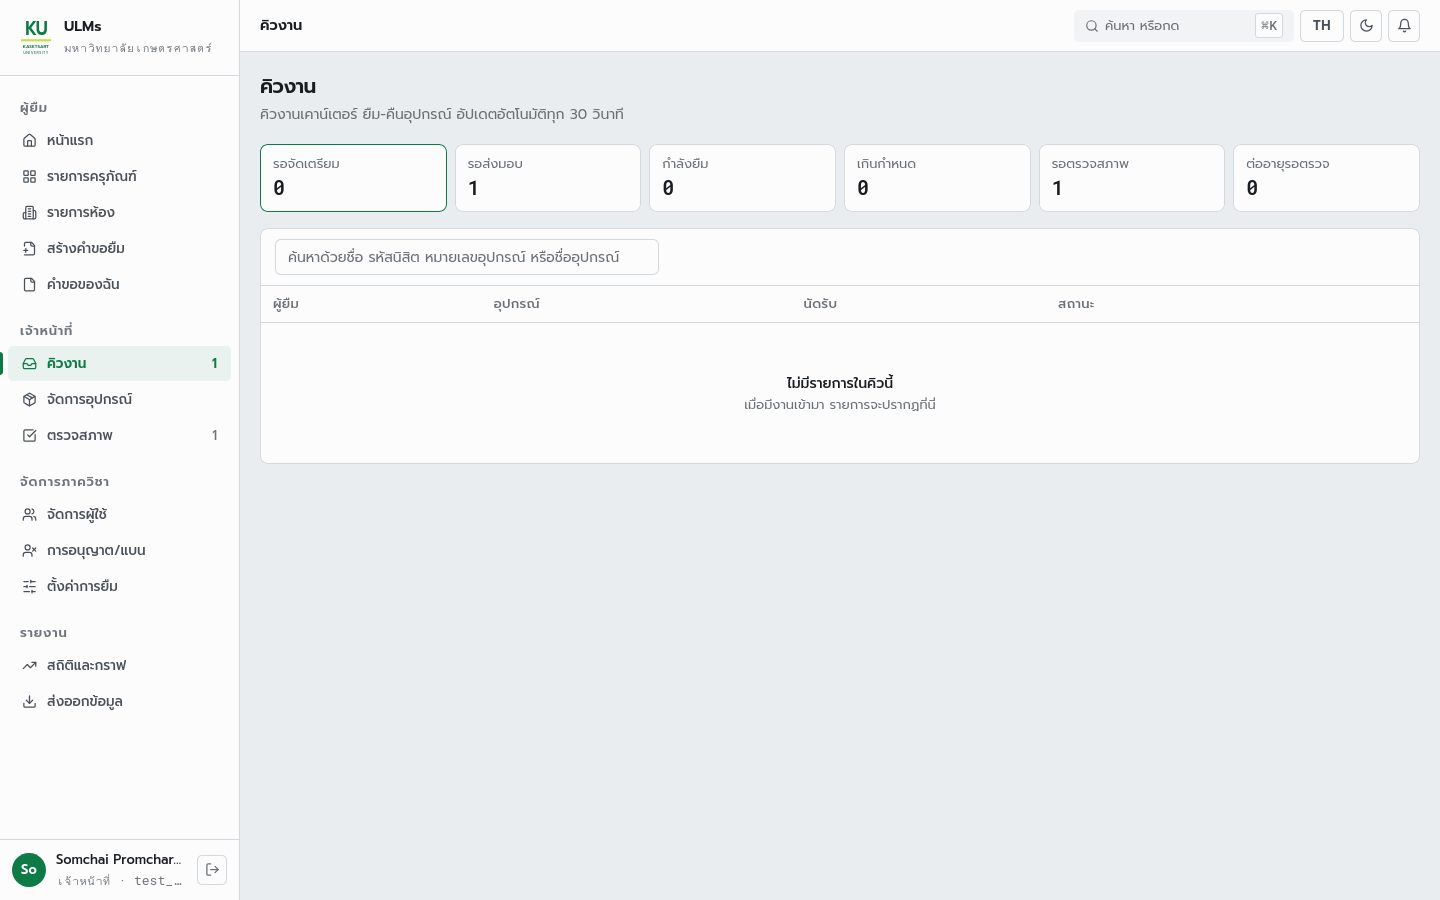
\includegraphics[width=\linewidth, trim={240 430 0 60}, clip]{audit/s-queue}\\[2pt]
{\sansall\scriptsize \rstf{} คิวงาน ``รอส่งมอบ 1'' ปุ่มส่งมอบเรียก \code{loan.confirmPickup} จริง}
\end{minipage}\hfill
\begin{minipage}[t]{0.49\textwidth}\centering
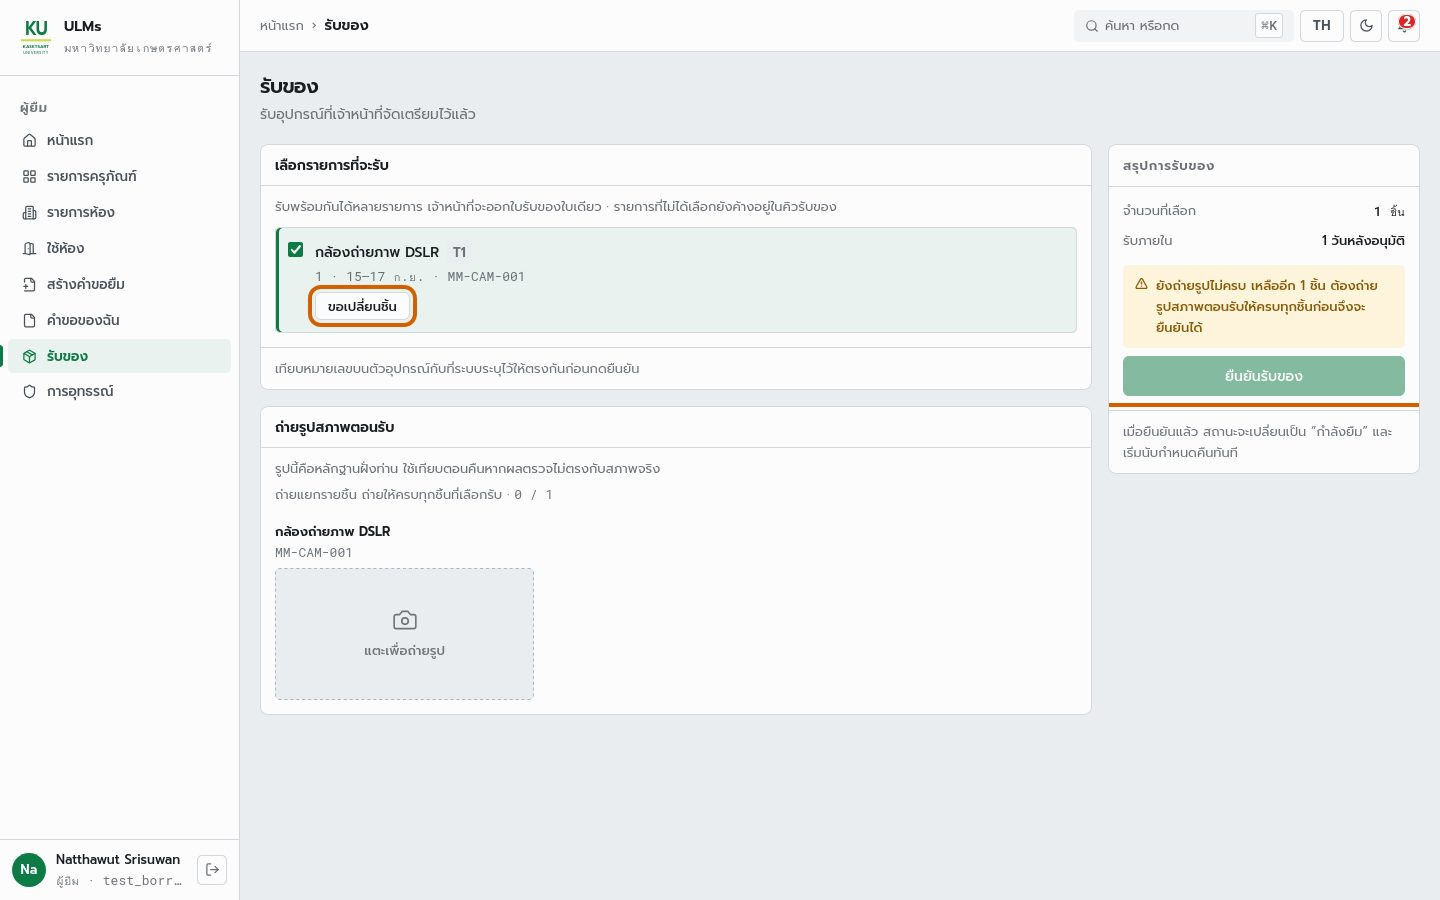
\includegraphics[width=\linewidth, trim={240 180 0 60}, clip]{audit/b-pickup}\\[2pt]
{\sansall\scriptsize \rbor{} หน้ารับของ บังคับถ่ายรูปก่อนกด ``ยืนยันรับของ'' แต่ไม่ส่งอะไรออกไป}
\end{minipage}
\caption{สองหน้าจอ ถ่ายจากระบบเดียวกันเวลาเดียวกัน ของชิ้นเดียวกัน}
\end{figure}

\fstep{แผนว่าไว้}
\begin{itemize}
\item FR-PKP-02 (สูง) \emph{``Borrower ต้องยืนยันการรับอุปกรณ์และตรวจสอบ Serial Number ก่อนกดยืนยัน''}
\item FR-PKP-03 (สูง) \emph{``ระบบต้องบังคับให้ Borrower อัปโหลดรูปถ่ายอุปกรณ์ตอนรับก่อนกดยืนยัน''}
\item SDS ตารางสถานะ: \code{Prepared} $\to$ \code{Lended} ผู้ทำคือผู้ยืม
\item BPMN กระบวนการยืม: ผู้ยืม ``ถ่ายรูปอุปกรณ์ตอนรับ + อัปโหลดเข้าระบบ'' (\code{bpmn\_data.py:49}) แล้วระบบจึงตั้งสถานะกำลังใช้งาน
\end{itemize}

\fstep{ระบบทำจริง}
\begin{table}[H]
\centering\small
\begin{tabular}{L{1.3cm}L{6.4cm}L{6.6cm}}
\toprule
\sansall\bfseries ผู้ทำ & \sansall\bfseries คำสั่ง (S4) & \sansall\bfseries ผล \\
\midrule
\rbor & \code{loan.confirmPickup} & 403 \code{ROLE\_NOT\_ALLOWED} --- ผู้ยืมไม่มีคำสั่งยืนยันรับของเลย \\
\rbor & \code{image.requestUpload} (ขอที่อัปโหลดรูป) & 403 \code{ROLE\_NOT\_ALLOWED} --- อัปโหลดได้เฉพาะเจ้าหน้าที่ (\code{image.router.ts:22}) \\
\rstf & \code{loan.confirmPickup} & สำเร็จ \code{status=Lended} ไม่มีช่องรับรูป \\
\bottomrule
\end{tabular}
\end{table}

คอมเมนต์ของ \code{confirmPickupInput} (\code{loan.schema.ts:201}) ยังเขียนตามแผนเดิม
\emph{``No image is uploaded here. Photos ... are attached by the borrower's own confirmation step''}
แต่ขั้นยืนยันของผู้ยืมที่อ้างถึงไม่มีอยู่ ผลคือตาราง \code{Images} ในฐานข้อมูลทดสอบมี\textbf{ 0 แถว} หลังการยืมครบวงจรไปแล้ว 3 ครั้ง

% -----------------------------------------------------------------------------
\section{รูปตอนรับของเป็นหลักฐานของใคร}
\label{sec:pickupphoto}
% -----------------------------------------------------------------------------
\fmeta{F05c (คำตัดสิน)}{dev ข้อ 5}{BE · FE · SA}

ข้อคิดเห็นของ dev แก้ปัญหา ``ยืนยันซ้ำสองที่'' ด้วยการตัดฝั่งผู้ยืมทิ้ง ซึ่งง่ายที่สุดในเชิงโค้ด แต่ตัดสิ่งที่แผนตั้งใจไว้ออกไปด้วย

\begin{warnbox}[title={ถ้าตัดรูปตอนรับทิ้ง อะไรพังต่อ}]
\begin{itemize}
\item FR-RTN-02 ให้เจ้าหน้าที่ \textbf{เปรียบเทียบรูปตอนรับกับตอนคืน} ถ้าไม่มีรูปตอนรับ ไม่มีอะไรให้เทียบ
\item FR-APL-03 ให้อาจารย์เห็นรูปก่อน--หลังตอนตัดสินอุทธรณ์ รูปตอนรับคือ\textbf{หลักฐานเดียวของผู้ยืม}ว่ารอยนั้นมีมาก่อน
      หน้าอุทธรณ์ฝั่งอาจารย์ (แม้ยังเป็นข้อมูลตัวอย่าง) ก็ออกแบบช่อง ``ตอนรับของ'' ไว้แล้ว
\item เกณฑ์ของอาจารย์: ถ้าเจ้าหน้าที่ยืนยันเองและถ่ายรูปเองทุกจุด ผู้ยืมไม่มีบทบาทในการส่งมอบเลย
\end{itemize}
\end{warnbox}

\begin{figure}[H]
\centering
\begin{tikzpicture}[x=1cm,y=1cm, box/.style={blk, text width=2.6cm, minimum height=10mm}]
  \node[tag, anchor=west] at (-0.2,1.0) {ตามโค้ดตอนนี้};
  \node[box, fill=rstf!8, draw=rstf!45] (a1) at (1.2,0) {จัดเตรียม};
  \node[box, fill=rstf!8, draw=rstf!45] (a2) at (4.4,0) {กดส่งมอบ\\\scriptsize\color{muted}\code{Lended} ทันที};
  \node[box, fill=rule!30, draw=rule, text=muted] (a3) at (7.6,0) {ผู้ยืมถ่ายรูป กดยืนยัน\\\scriptsize หายเมื่อรีเฟรช};
  \node[box, fill=rstf!8, draw=rstf!45] (a4) at (10.8,0) {รับคืน ไม่มีรูป};
  \draw[ar] (a1)--(a2); \draw[ar] (a2)--(a4.west); \draw[ar, dashed, draw=rule] (a2.south) |- ++(0,-0.5) -| (a3.south);
  \node[tag, anchor=west] at (-0.2,-1.6) {ข้อเสนอ (ตรงกับ BPMN)};
  \node[box, fill=rstf!8, draw=rstf!45] (b1) at (1.2,-2.6) {จัดเตรียม};
  \node[box, fill=rbor!10, draw=rbor!55] (b2) at (4.4,-2.6) {ผู้ยืมตรวจของ\\ถ่ายรูป กดยืนยัน};
  \node[box, fill=rstf!8, draw=rstf!45] (b3) at (7.6,-2.6) {กดส่งมอบ\\\scriptsize\color{muted}ต้องมีรูปผู้ยืมก่อน};
  \node[box, fill=rstf!8, draw=rstf!45] (b4) at (10.8,-2.6) {รับคืน + ถ่ายรูป};
  \draw[ar] (b1)--(b2); \draw[ar] (b2)--(b3); \draw[ar] (b3)--(b4);
  \node[lbl, below=1mm of b2, text width=3cm] {รูปตอนรับ = หลักฐานฝั่งผู้ยืม};
  \node[lbl, below=1mm of b4, text width=3cm] {รูปตอนคืน = หลักฐานฝั่งเจ้าหน้าที่};
\end{tikzpicture}
\caption{ข้อเสนอให้รูปสองจุดมาจากสองฝ่ายที่เป็นอิสระต่อกัน เจ้าหน้าที่ยังเป็นคนกดส่งมอบตามที่ dev ต้องการ แต่กดได้หลังผู้ยืมยืนยันแล้วเท่านั้น}
\end{figure}

\fstep{คำตัดสิน}
\vno{} ปัญหาที่ dev ชี้ (ยืนยันซ้ำ) มีจริง แต่ทางแก้ต้องไม่ใช่การตัดรูปตอนรับ

\fstep{ข้อเสนอ}
\begin{itemize}
\item \textbf{BE} เพิ่มคำสั่งฝั่งผู้ยืม เช่น \code{loan.confirmReceipt(\{ usageKey, imageUrls \})} บันทึกลงตาราง \code{Images}
      เป็น \code{BeforePicture} (ชนิดนี้มีอยู่แล้วใน \en{enum} \code{SubmissionType} ไม่ต้องเพิ่มตาราง)
\item \textbf{BE} \code{confirmPickup} ของเจ้าหน้าที่ปฏิเสธถ้ายังไม่มี \code{BeforePicture} ของการยืมนั้น ไม่ต้องเพิ่มสถานะใหม่
\item \textbf{BE} \code{image.requestUpload} ลดเป็นผู้ใช้ที่ล็อกอิน แล้วตรวจตามจุดประสงค์ ผู้ยืมอัปโหลดได้เฉพาะของการยืมของตัวเอง
      (คอมเมนต์ใน \code{image.router.ts} วางแผนเรื่องนี้ไว้แล้ว)
\item \textbf{FE} หน้ารับของต่อคำสั่งใหม่ คิวงานเจ้าหน้าที่แสดงว่า ``รอผู้ยืมยืนยัน'' หรือ ``ยืนยันแล้ว''
\item \textbf{SA} คง FR-PKP-02/03 เพิ่มขั้น ``เจ้าหน้าที่กดส่งมอบหลังผู้ยืมยืนยัน'' ลงใน FR-PKP และตารางสถานะของ SDS
\end{itemize}

% -----------------------------------------------------------------------------
\section{ปุ่มขอเปลี่ยนชิ้นของ T1 ยังต้องมีหรือไม่}
\label{sec:swap}
% -----------------------------------------------------------------------------
\fmeta{F05d}{dev ข้อ 5 ``ของ T1 ไม่มีกดขอเปลี่ยนของ (staff)''}{FE · SA}

\fstep{แผนว่าไว้}
FR-PKP-04 (กลาง) \emph{``สำหรับ T1 Borrower ต้องสามารถขอเปลี่ยนอุปกรณ์ตอนรับได้หากพบปัญหา''}
และข้อตัดสินของทีม: T1 ไม่มี serial การเปลี่ยนชิ้นทำกับเจ้าหน้าที่ตรงหน้าเคาน์เตอร์ ไม่บันทึก

\fstep{ระบบทำจริง}
\begin{figure}[H]
\centering
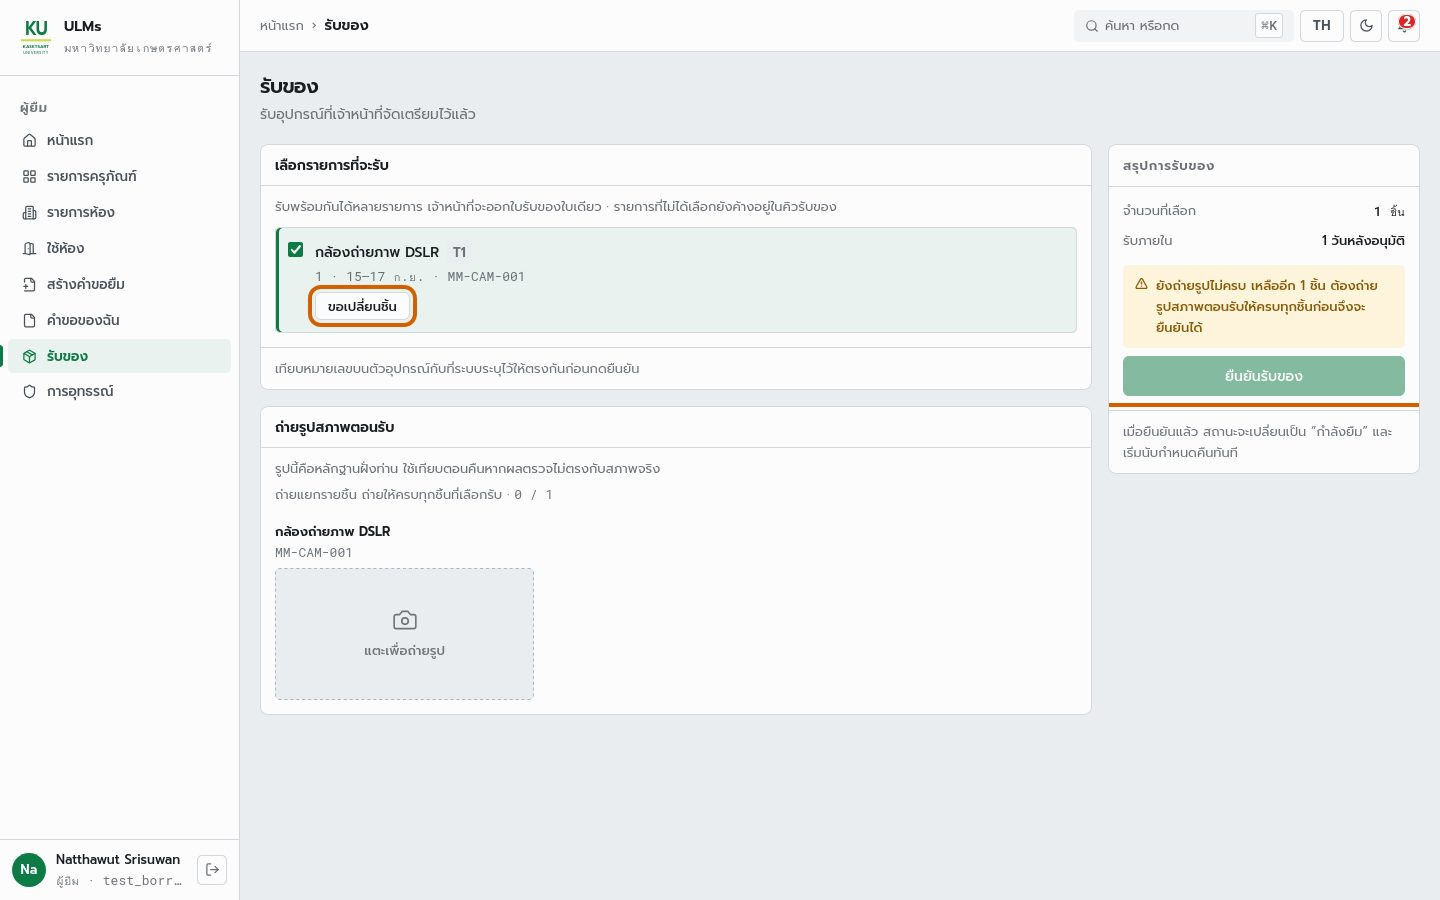
\includegraphics[width=0.6\textwidth, trim={260 510 340 140}, clip]{audit/b-pickup}
\caption{ปุ่ม ``ขอเปลี่ยนชิ้น'' มีอยู่ในหน้ารับของของผู้ยืม (\code{pickup-page.tsx:197} \code{canSwap = row.tier === "T1"}) ทำงานแค่ในหน้าจอ
ส่วน \en{backend} มี \code{loan.swapUnit} สำหรับเจ้าหน้าที่ แต่ไม่มีหน้าจอใดเรียก}
\end{figure}

\begin{keybox}[title={ข้อตัดสินทำให้คำถามนี้หายไปเอง}]
เมื่อ T1 ไม่มี serial ชิ้นทุกชิ้นของประเภทเดียวกันแทนกันได้ในสายตาระบบ เปลี่ยนตัวที่เคาน์เตอร์แล้ว
ข้อมูลในระบบยังถูกต้องทุกช่อง (ประเภท จำนวน ผู้ยืม วันคืน) จึงไม่มีอะไรต้องบันทึก
และไม่ต้องมีปุ่มทั้งฝั่งผู้ยืมและฝั่งเจ้าหน้าที่
\end{keybox}

\fstep{คำตัดสิน}
\vdec[ไม่ต้องมีปุ่ม]

\fstep{ข้อเสนอ}
FE ลบปุ่มขอเปลี่ยนชิ้นในหน้ารับของ · BE ตัดสินว่าจะเก็บ \code{loan.swapUnit} ไว้หรือลบ ·
SA ตัด FR-PKP-04 หรือเขียนใหม่ว่าเปลี่ยนนอกระบบ

\clearpage
% =============================================================================
\part{คืน ตรวจสภาพ และเครดิต}
% =============================================================================

\textbf{คำถามที่ภาคนี้ตอบ: ตอนของกลับมา ระบบมีหลักฐานพอให้ตัดสินความเสียหายหรือไม่ และบทลงโทษที่ออกมาทำงานตามกฎเครดิตหรือเปล่า}

% -----------------------------------------------------------------------------
\section{รูปตอนคืนของ ใครถ่าย}
\label{sec:returnphoto}
% -----------------------------------------------------------------------------
\fmeta{F05b}{dev ข้อ 5 ``รับรูปตอนคืนของ (staff)''}{BE · FE · SA}

\fstep{ตัวอย่าง}
นิสิตคืนคาลิปเปอร์ เจ้าหน้าที่เปิดหน้าตรวจสภาพเพื่อเทียบรูปก่อนและหลัง แล้วให้ระดับความเสียหาย

\fstep{แผนว่าไว้ --- สองเอกสารพูดต่างกัน}
\begin{itemize}
\item SRS FR-RTN-01 (สูง) \emph{``Borrower ต้องสามารถแจ้งคืนผ่านระบบพร้อมอัปโหลดรูปถ่ายตอนคืน''} --- ผู้ยืมถ่าย
\item BPMN กระบวนการคืน เลนเจ้าหน้าที่ \emph{``ถ่ายรูปอุปกรณ์ตอนคืน + อัปโหลดเข้าระบบ''} (\code{bpmn\_data.py:153}) --- เจ้าหน้าที่ถ่าย
\end{itemize}

\fstep{ระบบทำจริง}
\begin{figure}[H]
\centering
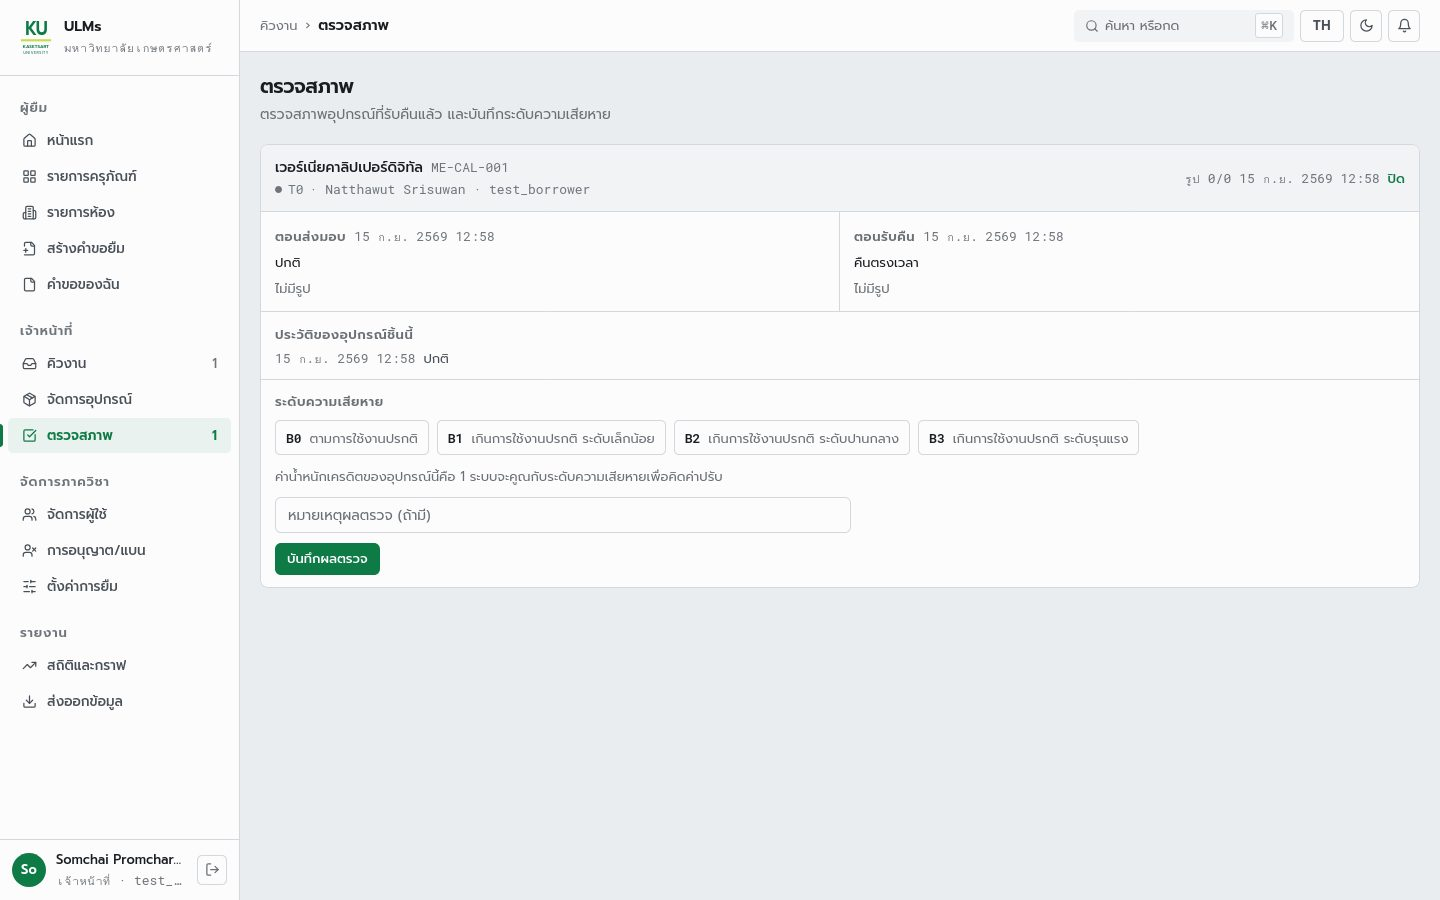
\includegraphics[width=0.95\textwidth, trim={240 300 0 60}, clip]{audit/s-inspection}
\caption{หน้าตรวจสภาพ ของที่รับคืนแล้ว ``ตอนส่งมอบ ไม่มีรูป'' ``ตอนรับคืน ไม่มีรูป'' มุมขวาบน ``รูป 0/0''
และฟอร์มให้ระดับความเสียหายไม่มีช่องแนบรูป}
\end{figure}

ไม่มีจุดใดในระบบเขียนรูปตอนคืน \code{recordReturnInput} (\code{loan.schema.ts:222}) รับแค่ \code{usageKey} กับ \code{note}
ส่วน \code{inspection.create} รับ \code{imageUrls} ได้ แต่หน้าตรวจสภาพส่งแค่ \code{usageKey level note}
(\code{inspection-page.tsx:175-179})

\fstep{คำตัดสิน}
\vok[ถูก แก้ SRS] ข้อคิดเห็นตรงกับ BPMN และสมเหตุสมผลกว่า SRS เพราะของคืนที่เคาน์เตอร์ต่อหน้าเจ้าหน้าที่
รวมกับข้อเสนอในหัวข้อ~\ref{sec:pickupphoto} ทำให้รูปสองจุดมาจากสองฝ่าย

\fstep{ข้อเสนอ}
\begin{itemize}
\item \textbf{BE} \code{recordReturn} รับ \code{imageUrls} บันทึกเป็น \code{AfterPicture} (ใช้ตาราง \code{Images} เดิม)
\item \textbf{FE} ปุ่มรับคืนในคิวงานเปิดกล้องก่อนยืนยัน หน้าตรวจสภาพแสดงรูปผู้ยืม (ก่อน) คู่รูปเจ้าหน้าที่ (หลัง) ตาม FR-RTN-02
\item \textbf{SA} แก้ FR-RTN-01 เป็นเจ้าหน้าที่ถ่ายรูปตอนรับคืน ผู้ยืมไม่ต้องแจ้งคืนผ่านระบบ
\end{itemize}

% -----------------------------------------------------------------------------
\section{รายการรอตรวจสภาพ และสถานะที่ไม่มีวันเกิด}
\label{sec:inspectq}
% -----------------------------------------------------------------------------
\fmeta{F05a · F08}{dev ข้อ 5 (ขีดทิ้ง) · ตรวจเจอเพิ่ม}{BE · FE}

dev ขีดข้อ ``ของค้างที่รอตรวจสภาพ (staff)'' ทิ้งเอง ซึ่งถูก รายการนี้มีแล้วทั้งในคิวงาน (ช่อง ``รอตรวจสภาพ 1'' ในภาพหัวข้อ~\ref{sec:handover})
และหน้าตรวจสภาพ (ภาพหัวข้อ~\ref{sec:returnphoto}) ดึงจาก \code{inspection.list} จริง \quad \vok[ขีดทิ้งถูก]

แต่ฝั่งผู้ยืมมีสองสถานะที่ไม่มีทางแสดง

\begin{table}[H]
\centering\small
\begin{tabular}{L{3.4cm}L{5.6cm}L{5.3cm}}
\toprule
\sansall\bfseries สถานะ & \sansall\bfseries มาจาก & \sansall\bfseries ทำไมไม่เกิด \\
\midrule
\code{preparing} ``กำลังจัดเตรียม'' & \code{loan.request.service.ts:585} แปลงจาก \code{UsageLog.CurrentStatus = Pending} & ไม่มีโค้ดใดเขียน \code{Pending} \code{allocate} สร้าง \code{Prepared} ทันที \\
\code{inspecting} ``รอตรวจสภาพ'' & \code{mock-data.ts:484} ฝั่ง FE & \en{backend} ไม่มีสถานะนี้ ส่ง \code{returned} มาแทน \\
\bottomrule
\end{tabular}
\end{table}

\fstep{คำตัดสิน}
F08 \vbad[ต้องแก้ ระดับต่ำ] ผู้ยืมไม่เห็นว่าของกำลังถูกตรวจ \quad
\fstep{ข้อเสนอ}
BE ตัด \code{preparing} ออกจากชุดสถานะ หรือให้มีขั้นจริง · FE แสดง \code{returned} เป็น ``รอตรวจสภาพ'' แล้วลบ \code{inspecting}

% -----------------------------------------------------------------------------
\section{บทลงโทษทำงานตรงกับกฎเครดิตหรือไม่}
\label{sec:penalty}
% -----------------------------------------------------------------------------
\fmeta{F17 · F25}{ตรวจเจอเพิ่ม (สองข้อแรกพบ 11 ก.ย. ยังไม่แก้)}{BE · FE}

\fstep{ตัวอย่าง}
นิสิตคืนออสซิลโลสโคประดับ B2 ได้โทษหักเครดิต ต่อมาเจ้าหน้าที่เปิดเมนู ``การอนุญาต/แบน'' แบนนิสิตคนนี้ 7 วัน
นิสิตส่งคำขอยืมไม่ได้ สามวันต่อมาเจ้าหน้าที่ยกเลิกแบน

\fstep{แผนว่าไว้}
\textbf{แผนไม่มีการแบนการยืม} บทลงโทษมีผลผ่านแถบเครดิตเท่านั้น คือจำกัดจำนวนวันยืมและเปลี่ยนเส้นทางการอนุมัติ
FR-CRD-04 อายุโทษ = discredit × 2 วัน · FR-CRD-06 \emph{``credit\_score ต้องคำนวณจากผลรวมของ Demerit Event ที่ยัง active เท่านั้น ไม่แก้ไขโดยตรง''}
· FR-CRD-08 สิทธิ์การยืมปรับตามแถบเครดิต D0--D3
ส่วน FR-ADM-03 \emph{``Admin ต้องสามารถระงับบัญชีผู้ใช้และคืนบัญชีได้''} คือปิดบัญชีทั้งบัญชี ซึ่งโค้ดทำด้วย \code{setUserActive} แยกต่างหาก

\fstep{ระบบทำจริง (ยืนยันจากโค้ด ยังไม่ได้รันสถานการณ์นี้)}
โค้ดมี\textbf{การแบนการยืม}ที่ไม่มีใน SRS: \code{admin.setUserBan} (\code{admin.router.ts:154} เจ้าหน้าที่ใช้ได้)
หน้า ``การอนุญาต/แบน'' ของเจ้าหน้าที่และอาจารย์ และ \code{loan.create} ปฏิเสธด้วย \code{BORROWING\_SUSPENDED}
(\code{loan.request.service.ts:142}) e2e test TP-ADM-E2E-05/06 ทดสอบการแบนนี้อยู่ และ SDS v1.1 เขียนการระงับการยืมตามโค้ดไว้
(\code{sds\_data.py:144} และ \code{:525}) ฟีเจอร์นี้ยังเพิ่มอำนาจให้เจ้าหน้าที่ ซึ่งสวนเกณฑ์สมดุลบทบาท (หัวข้อ~\ref{sec:roles})

ตาราง \code{PenaltyInfo} เก็บการแบนกับโทษเครดิตในแถวแบบเดียวกัน แต่ตัวกรองสามจุดแยกชนิดไม่เหมือนกัน

\begin{table}[H]
\centering\small
\begin{tabular}{L{3.0cm}L{2.7cm}L{2.7cm}L{2.6cm}L{2.0cm}}
\toprule
\sansall\bfseries ชนิดโทษ & \sansall\bfseries กันการยืม \scriptsize(\code{activeBanWhere}) & \sansall\bfseries ป้าย ``ถูกระงับ'' \scriptsize(\code{admin.schema.ts:18}) & \sansall\bfseries ยกเลิกแบน \scriptsize(\code{admin.service.ts:450}) & \sansall\bfseries ตรงแผนไหม \\
\midrule
แบน โดยเจ้าหน้าที่/ผู้ดูแล \scriptsize(ไม่มี \code{UsageKey}) & กัน & ขึ้น & ปิดโทษ & \textcolor{bad}{ไม่มีในแผน} \\
โทษความเสียหาย/คืนช้า \scriptsize(\code{penalty.service.ts:179}) & ไม่กัน \scriptsize(ตาม FR-CRD-08 ถูก) & \textcolor{bad}{ขึ้น} & \textcolor{bad}{ปิดโทษด้วย} & \textcolor{bad}{ผิด 2 จุด} \\
\bottomrule
\end{tabular}
\end{table}

\begin{lstlisting}
// backend/src/admin/admin.service.ts:450  setUserBan({ banned: false })
await this.prisma.penaltyInfo.updateMany({
  where: { AccountKey: input.id, ...activePenaltyWhere() },   // every active penalty, damage included
  data: { InEffect: false },
});
// backend/src/common/schemas/penalty.schema.ts:72
export function activeBanWhere() {
  return { ...activePenaltyWhere(), UsageKey: null, CreditDeducted: null };  // bans only
}
\end{lstlisting}

อีกสองจุดในหมวดเดียวกัน
\begin{itemize}
\item เครดิตถูกลบตรงที่ \code{AccountInfo.UserCredit} (\code{penalty.service.ts:198} \code{decrement}) ไม่ได้คำนวณจากโทษที่ยัง \en{active}
      ตาม FR-CRD-06 ผลคือโทษที่ถูกปิด (ด้วยการยกแบนหรือการอุทธรณ์) ไม่คืนเครดิตให้เอง
\item ปฏิเสธคำขอแล้วเหตุผลของผู้ยืมถูกเขียนทับด้วยเหตุผลที่ปฏิเสธ (\code{approval.service.ts:253} \code{Reason: input.reason ?? row.Reason})
\end{itemize}

\fstep{คำตัดสิน}
F17 \vbad{} \quad F25 \vbad[ต้องแก้ ระดับต่ำ] เจ้าหน้าที่เห็นว่านิสิต ``ถูกระงับ'' ทั้งที่นิสิตยังยืมได้

\fstep{ข้อเสนอ}
\begin{itemize}
\item \textbf{BE/FE} ลบการแบนการยืมที่ไม่มีในแผน (\code{setUserBan} \code{assertNotBanned} หน้า ``การอนุญาต/แบน'' และ e2e ที่เกี่ยวข้อง)
      ถ้าทีมตัดสินคงไว้ ต้องเพิ่มเข้า SRS และยกเลิกแบนต้องใช้ \code{activeBanWhere()} แทน \code{activePenaltyWhere()}
\item \textbf{BE/FE} ป้ายสถานะผู้ใช้แสดงแถบเครดิตและโทษที่ยังมีผล แทน ``ถูกระงับ''
\item \textbf{SA} แก้ SDS v1.1 ส่วนที่เขียนการระงับการยืมไว้ตามโค้ด
\item \textbf{BE} เก็บเหตุผลที่ปฏิเสธแยกจากเหตุผลของผู้ยืม ถ้าต้องเพิ่มคอลัมน์ต้องผ่าน BE-lead ระหว่างนี้ส่งในการแจ้งเตือนได้
\item \textbf{SA} ตัดสินว่า FR-CRD-06 (คำนวณจากโทษที่ \en{active}) ยังต้องการหรือไม่ ถ้าต้องการ การปิดโทษต้องคำนวณเครดิตใหม่
\end{itemize}

% -----------------------------------------------------------------------------
\section{อุทธรณ์ทำได้แค่ไหน}
\label{sec:appeal}
% -----------------------------------------------------------------------------
\fmeta{F18 (อุทธรณ์)}{ตรวจเจอเพิ่ม}{BE · FE}

\begin{figure}[H]
\centering
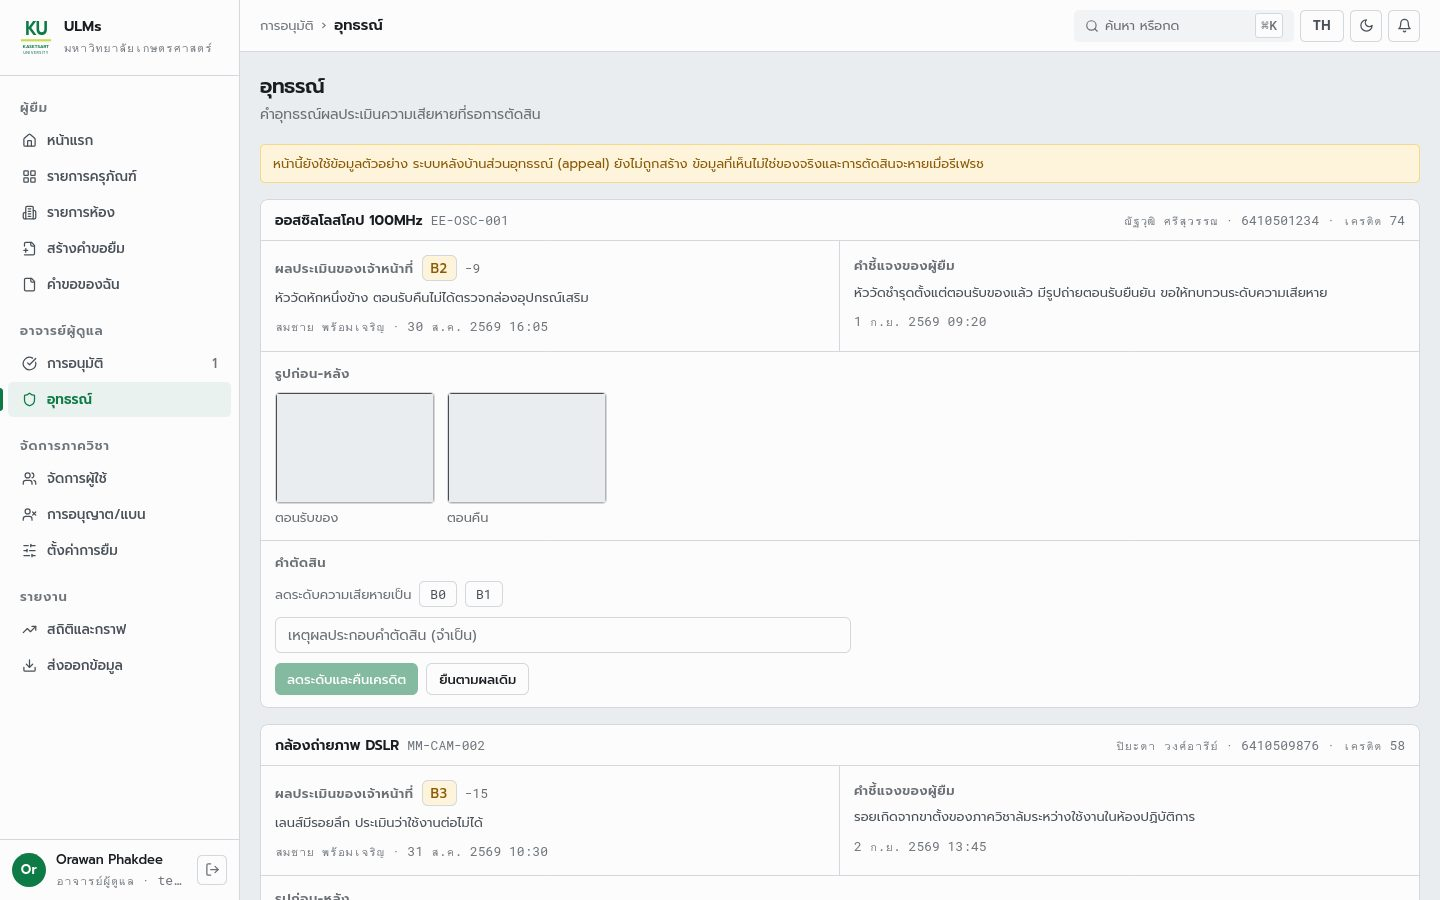
\includegraphics[width=0.95\textwidth, trim={240 380 0 60}, clip]{audit/v-appeals-mock}
\caption{หน้าอุทธรณ์ของอาจารย์ แถบเหลืองด้านบนบอกเองว่า ``หน้านี้ยังใช้ข้อมูลตัวอย่าง ระบบหลังบ้านส่วนอุทธรณ์ยังไม่ถูกสร้าง''}
\end{figure}

\en{backend} ไม่มี \en{router} อุทธรณ์ แม้ตาราง \code{AppealInfo} จะมีแล้ว หน้าส่งอุทธรณ์ของผู้ยืมก็เก็บในหน่วยความจำ (F07)
FR-APL-01 ถึง FR-APL-06 จึงยังไม่มีข้อใดทำงาน ข้อนี้กระทบเกณฑ์ของอาจารย์โดยตรง เพราะอุทธรณ์คืองานหลักอย่างหนึ่งของบทบาทอาจารย์ (หัวข้อ~\ref{sec:roles})

\fstep{คำตัดสิน}
\vbad{} \quad
\fstep{ข้อเสนอ}
BE สร้าง \en{router} อุทธรณ์ ( \code{create list getById decide} ตามชื่อที่ FE ประกาศไว้แล้ว) ผู้ตัดสินต้องไม่ใช่ผู้ประเมินเดิม (FR-APL-04)
ผ่านแล้วปิดโทษและคืนเครดิต (FR-APL-05) · FE ต่อสองหน้าที่มีอยู่

\clearpage
% =============================================================================
\part{ห้อง T3}
% =============================================================================

\textbf{คำถามที่ภาคนี้ตอบ: กฎของห้องที่ทีมตกลงแล้ว มีข้อมูลรองรับและถูกบังคับจริงหรือไม่}

% -----------------------------------------------------------------------------
\section{ห้องจุได้กี่คน}
\label{sec:capacity}
% -----------------------------------------------------------------------------
\fmeta{F02}{dev ข้อ 2 ``backend ไม่มีความจุห้อง T3''}{BE-lead · SA}

\fstep{แผนว่าไว้}
FR-EQP-04 (สูง) \emph{``Staff ต้องสามารถลงทะเบียนสถานที่ (T3) พร้อมกำหนดจำนวนที่นั่ง ความยาวสล็อต และช่วงเวลาเปิดใช้''}

\fstep{ระบบทำจริง}
\begin{figure}[H]
\centering
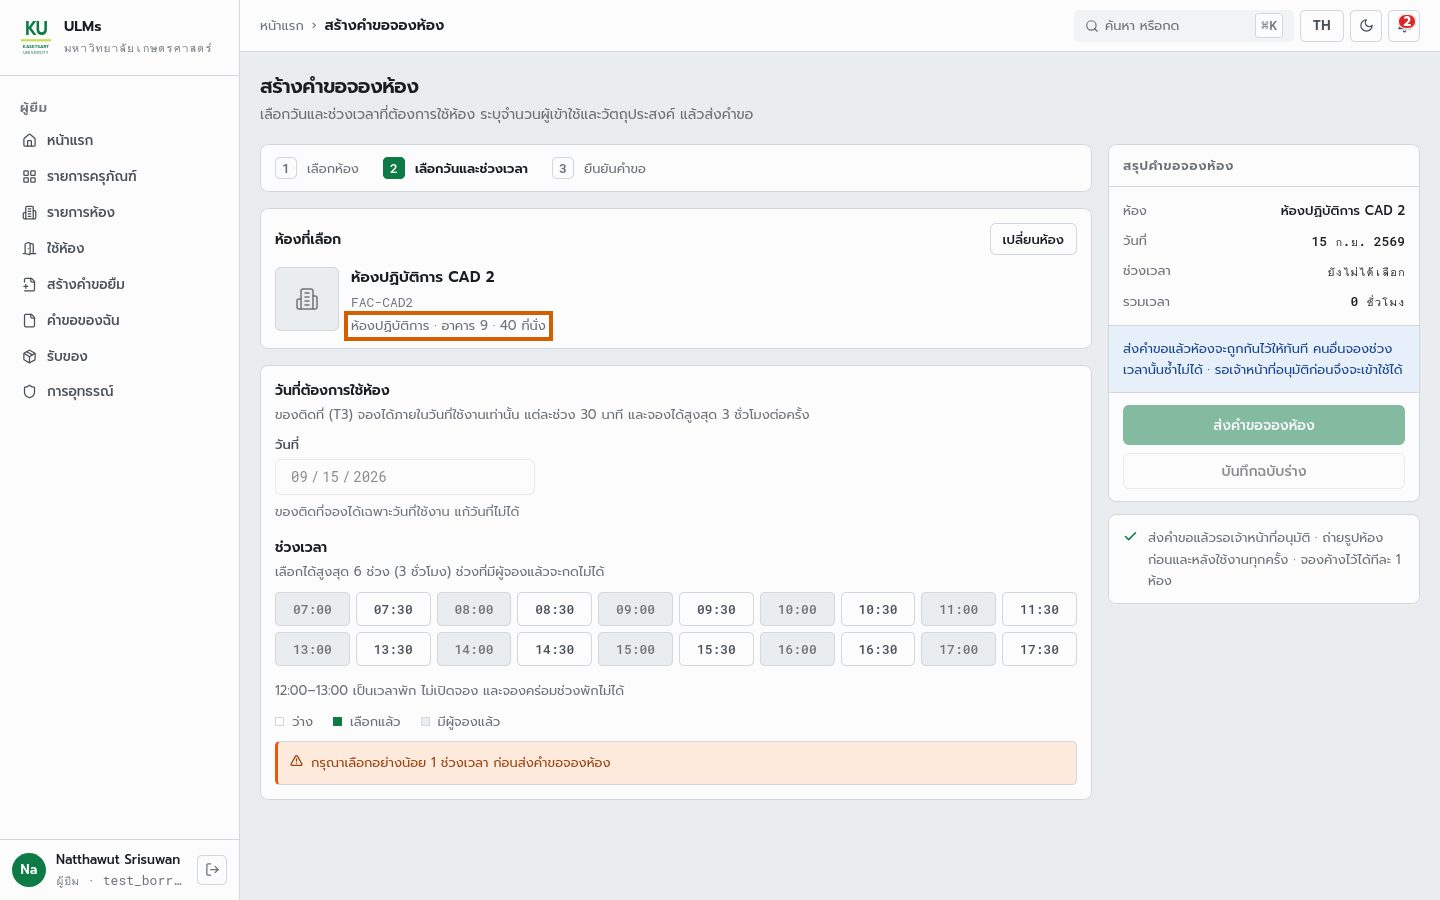
\includegraphics[width=0.95\textwidth, trim={240 90 0 60}, clip]{audit/b-room-booking}
\caption{หน้าจองห้องแสดง ``40 ที่นั่ง'' และช่องเวลา 30 นาที 07:00--17:30 ครบตามข้อตัดสิน แต่ข้อมูลทั้งหน้ามาจาก \code{mock-data.ts} ไม่ใช่ฐานข้อมูล}
\end{figure}

ห้องที่สร้างผ่าน \code{item.createRoom} ใน S3 ได้กลับมาแค่ช่องเหล่านี้ ไม่มีความจุ ความยาวช่อง หรือเวลาเปิด
\begin{lstlisting}
item.createRoom -> { condition, creditWeight, description, imageUrl, lendable, location,
                     managementGroup, name, resourceKey, roomKey, status, tier }
\end{lstlisting}
ตาราง \code{RoomInfo} (\code{schema.prisma:281}) มีแค่ชื่อ คำอธิบาย ที่ตั้ง รูป และน้ำหนักเครดิต ทั้ง ER และ SDS ก็ไม่มีช่องนี้

\begin{warnbox}[title={ต้องตัดสินก่อนเพิ่มคอลัมน์ --- ความจุใช้ทำอะไร}]
หน้าจอและ \en{backend} ตอนนี้จองห้องแบบ\textbf{ทั้งห้อง} (ช่องที่มีคนจองแล้วกดไม่ได้ S3 ข้อ R7 ชนถูกปฏิเสธ)
ส่วนข้อเสนอโครงการยกตัวอย่าง ``ห้อง 7603 จะมีที่ว่าง 2 ที่ ในเวลา 14:00'' ซึ่งเป็นการจอง\textbf{รายที่นั่ง}
ถ้าจองทั้งห้อง ความจุเป็นข้อมูลให้เลือกห้องและตรวจ ``จำนวนผู้เข้าใช้ $\le$ ความจุ'' ถ้าจองรายที่นั่ง
กฎกันซ้อนทั้งหมดต้องเปลี่ยน แนะนำแบบทั้งห้องตามที่ทำอยู่
\end{warnbox}

\fstep{คำตัดสิน}
\vok{}
\fstep{ข้อเสนอ}
\textbf{BE-lead} เพิ่ม \code{RoomInfo.Capacity} (และเวลาเปิด--ปิด ถ้าไม่ใช้ค่ากลางทั้งระบบ) ไม่ต้องเพิ่มความยาวช่อง เพราะทีมตัดสินเป็น 30 นาทีทุกห้อง
· \textbf{SA} แก้ FR-EQP-04 ให้ความยาวช่องเป็นค่ากลาง และระบุว่าจองทั้งห้อง

% -----------------------------------------------------------------------------
\section{ช่องละ 30 นาที ต่อกันไม่เกิน 6 ช่อง --- ใครบังคับกฎนี้}
\label{sec:slots}
% -----------------------------------------------------------------------------
\fmeta{F03 · F10}{dev ข้อ 3 ``List slot เวลายืมห้อง T3 เก็บว่าง/ไม่ว่าง'' · ตรวจเจอเพิ่ม}{BE · FE · SA}

\fstep{แผนว่าไว้ --- สามชั้นพูดคนละเลข}
\begin{table}[H]
\centering\small
\begin{tabular}{L{4.6cm}L{9.7cm}}
\toprule
\sansall\bfseries ที่ & \sansall\bfseries กฎ \\
\midrule
ข้อตัดสินของทีม & ช่องละ 30 นาที ต่อกันไม่เกิน 6 ช่อง \\
SRS FR-REQ-08 & \textcolor{bad}{รายชั่วโมง จองพร้อมกันสูงสุด 2 สล็อต} · FR-RSV-02 จองได้เฉพาะวันเดียวกัน \\
หน้าจองห้อง (FE) & 30 นาที สูงสุด 6 ช่อง ต่อเนื่อง วันเดียวกัน 07:00--18:00 เว้น 12:00--13:00 --- ตรงข้อตัดสิน \\
ค่าคงที่ FE & \code{MAX\_T3\_CONCURRENT\_SLOTS: 2} ยังค้าง และ \code{test:ac} ข้อ 2.6 ยังทดสอบว่า ``จองช่องที่ 3 ไม่ได้'' \\
\en{backend} & \textcolor{bad}{ไม่มีกฎใดเลย} นอกจากกันซ้อน \\
\bottomrule
\end{tabular}
\end{table}

\fstep{ระบบทำจริง}
S3 ส่งคำขอจองห้องตรงเข้า \en{API} (เหมือนหน้าจออื่นหรือสคริปต์ที่ข้ามหน้าจองห้อง) แล้วเทียบกับกฎ

\begin{table}[H]
\centering\small
\begin{tabular}{L{5.8cm}L{3.7cm}L{4.8cm}}
\toprule
\sansall\bfseries คำขอ & \sansall\bfseries ผิดกฎข้อไหน & \sansall\bfseries \en{backend} ตอบ \\
\midrule
R1 พรุ่งนี้ 09:00--09:30 & วันเดียวกัน & \textcolor{bad}{รับ} \code{pending} \\
R2 พรุ่งนี้ 09:15--09:45 & นอกกริด · ซ้อน R1 & ปฏิเสธ \code{WINDOW\_NOT\_AVAILABLE} (เพราะซ้อน) \\
R3 พรุ่งนี้ 13:10--13:40 & นอกกริด & \textcolor{bad}{รับ} \\
R4 พรุ่งนี้ 14:00--17:30 (7 ช่อง) & เกิน 6 ช่อง & \textcolor{bad}{รับ} \\
R4b อีก 2 วัน 09:00--12:00 (6 ช่อง) & วันเดียวกัน & \textcolor{bad}{รับ} \\
R5 พรุ่งนี้ 22:00 ถึงตี 1 & นอกเวลาเปิด · ข้ามวัน & \textcolor{bad}{รับ} \\
R6 อีก 5 วัน 09:00--10:00 & วันเดียวกัน & \textcolor{bad}{รับ} \\
R7 คนอื่นขอ 09:00--09:30 ซ้ำ R1 & ซ้อน & ปฏิเสธ \code{WINDOW\_NOT\_AVAILABLE} \\
\bottomrule
\end{tabular}
\caption{ผลรันจริงจาก \code{results/s3\_rooms.json} ปฏิเสธ 2 ใน 8 และทั้งสองครั้งเพราะช่วงซ้อนเท่านั้น}
\end{table}

ส่วนช่อง ``ว่าง/ไม่ว่าง'' ที่หน้าจอแสดง มาจากค่าสมมติ (\code{mock-data.ts:352} TODO \code{GET /facilities/:id/slots})

\begin{warnbox}[title={``เก็บว่าง/ไม่ว่าง'' ไม่ควรเป็นตารางใหม่}]
ความว่างของช่องคำนวณได้จาก \code{Reservations} ที่มีอยู่ (มี \en{index} \code{ResourceKey, StartTime, EndTime} แล้ว)
ถ้าเก็บเป็นตาราง slot แยก จะมีความจริงสองชุดที่ต้องทำให้ตรงกันทุกครั้งที่จอง ยกเลิก หรือหมดอายุ
ซึ่งเป็นปัญหาแบบเดียวกับตัวนับในหัวข้อ~\ref{sec:counter} และการเพิ่มตารางต้องผ่าน BE-lead ด้วย
\end{warnbox}

\fstep{คำตัดสิน}
F03 \vpart{} ต้องมี \en{API} รายการช่องจริง แต่ไม่ต้องเก็บ \quad F10 \vbad{}

\fstep{ข้อเสนอ}
\begin{itemize}
\item \textbf{BE} \code{loan.create} สำหรับห้อง ตรวจ: นาทีหาร 30 ลงตัว · ยาว $\le$ 180 นาที · วันเดียวกันตามเวลาไทย · อยู่ในเวลาเปิดไม่คร่อมพักเที่ยง · วันเริ่มคือวันนี้
\item \textbf{BE} \en{query} \code{item.roomSlots(\{ resourceKey, date \})} คืน 20 ช่องพร้อมสถานะ คำนวณจาก \code{Reservations}
\item \textbf{FE} หน้าจองห้องใช้ \en{query} นี้แทนค่าสมมติ ลบ \code{MAX\_T3\_CONCURRENT\_SLOTS} และแก้ \code{test:ac} ข้อ 2.6
\item \textbf{SA} แก้ FR-REQ-08 เป็น ``ช่องละ 30 นาที ต่อเนื่องไม่เกิน 6 ช่องต่อการจอง''
\end{itemize}

% -----------------------------------------------------------------------------
\section{ห้องที่ลงทะเบียนใหม่ จองได้หรือไม่}
\label{sec:roomelig}
% -----------------------------------------------------------------------------
\fmeta{F23}{ตรวจเจอเพิ่ม}{BE}

\fstep{ระบบทำจริง}
S3 สร้างห้องด้วย \code{item.createRoom} แล้วให้ผู้ยืมจองทันที ได้ \code{NOT\_ELIGIBLE / NO\_RULES\_CONFIGURED}
แบบเดียวกับอุปกรณ์ในหัวข้อ~\ref{sec:register} แต่ต่างกันตรงที่ห้อง\textbf{ไม่มีคำสั่งให้เปิดสิทธิ์}
เพราะ \code{item.setEligibility} รับ \code{itemKey} ของประเภทอุปกรณ์เท่านั้น และห้องไม่มี \code{itemKey}

\begin{badbox}[title={ห้องที่เจ้าหน้าที่เพิ่มเอง ไม่มีใครจองได้ตลอดไป}]
การทดสอบกฎช่องเวลาใน S3 ต้องเขียนแถว \code{Eligibility} ลงฐานข้อมูลตรง (บันทึกไว้ในผลรันเป็น ``DB workaround'')
เพราะไม่มีทางอื่น ในระบบจริงห้องทุกห้องที่ไม่ได้มาจาก \en{seed} จะจองไม่ได้
\end{badbox}

\fstep{คำตัดสิน}
\vbad{}
\fstep{ข้อเสนอ}
BE ให้ \code{createRoom} รับชุดสิทธิ์ หรือเพิ่ม \code{item.setRoomEligibility(\{ resourceKey, rules \})}

\clearpage
% =============================================================================
\part{ตรวจตัดขวางทั้งระบบ}
% =============================================================================

\textbf{คำถามที่ภาคนี้ตอบ: เมื่อมองข้ามหน้าจอทีละหน้า ระบบทั้งชุดยังสอดคล้องกันเองหรือไม่}

% -----------------------------------------------------------------------------
\section{ทุกบทบาทมีงานที่ขาดไม่ได้จริงหรือไม่}
\label{sec:roles}
% -----------------------------------------------------------------------------
\fmeta{F19}{เกณฑ์ของอาจารย์}{SA}

\fstep{แผนว่าไว้}
อาจารย์กำหนดว่าทุกบทบาทต้องมีปฏิสัมพันธ์กัน ไม่มีบทบาทใดทำทุกอย่าง และไม่มีบทบาทใดแทบไม่มีงาน
ตารางนี้นับเฉพาะขั้นที่\textbf{ทำผ่านหน้าจอได้จริงวันนี้} เทียบกับขั้นหลังแก้ตามข้อเสนอในเล่มนี้

\begin{table}[H]
\centering\small
\begin{tabular}{L{3.4cm}L{5.4cm}L{5.5cm}}
\toprule
\sansall\bfseries ขั้น & \sansall\bfseries ทำได้จริงวันนี้ & \sansall\bfseries หลังแก้ตามข้อเสนอ \\
\midrule
ลงทะเบียนของ/ห้อง & ไม่มีหน้าจอ & \rstf \\
ส่งคำขอ & \textcolor{muted}{ผู้ยืมกดได้แต่ไม่ถึงระบบ} & \rbor \\
อนุมัติ & \rsys{} T0--T1 · \rsup{} T2 · \rstf{} T3 & \rsys{} T0--T1 · \rsup{} T1 D2--D3 และ T2 · \rstf{} T3 \\
จัดเตรียม & \rstf & \rstf \\
ส่งมอบ & \rstf{} คนเดียว & \rbor{} ยืนยัน+รูป แล้ว \rstf{} ส่งมอบ \\
รับคืน & \rstf{} ไม่มีรูป & \rbor{} นำมาคืน \rstf{} รับ+รูป \\
ตรวจสภาพ & \rstf{} (T2 คนละคนกับผู้เตรียม) & \rstf \\
หักเครดิต & \rsys & \rsys \\
อุทธรณ์ & \textcolor{muted}{ข้อมูลตัวอย่าง} & \rbor{} ยื่น \rsup{} ตัดสิน \\
จำหน่ายของที่เสีย & \textcolor{muted}{\code{NOT\_IMPLEMENTED}} & \rstf{} เสนอ \rsup{} อนุมัติ (FR-EQP-08) \\
ผู้ใช้ ตั้งค่า บันทึก & \radm & \radm \\
\bottomrule
\end{tabular}
\end{table}

\begin{figure}[H]
\centering
\begin{tikzpicture}[x=0.55cm, y=0.55cm]
  \node[tag, anchor=west] at (0,5.9) {ทำได้จริงวันนี้};
  \node[tag, anchor=west] at (13,5.9) {หลังแก้};
  \foreach \r/\name/\col/\now/\after [count=\i] in {
      1/ผู้ยืม/rbor/0/4, 2/เจ้าหน้าที่/rstf/7/7, 3/อาจารย์/rsup/1/3, 4/ผู้ดูแลระบบ/radm/1/1} {
    \pgfmathsetmacro{\yy}{5-\r*1.1}
    \node[lbl, anchor=east] at (0,\yy) {\name};
    \fill[\col] (0.2,\yy-0.35) rectangle ++(\now,0.7);
    \node[lbl, anchor=west] at (0.3+\now,\yy) {\now};
    \node[lbl, anchor=east] at (13,\yy) {\name};
    \fill[\col] (13.2,\yy-0.35) rectangle ++(\after,0.7);
    \node[lbl, anchor=west] at (13.3+\after,\yy) {\after};
  }
\end{tikzpicture}
\caption{จำนวนขั้นในตารางข้างบนที่แต่ละบทบาทลงมือเอง ผู้ยืมทำอะไรถึงระบบไม่ได้เลยในวันนี้ ส่วนเจ้าหน้าที่ทำเกือบทุกขั้น}
\end{figure}

\fstep{คำตัดสิน}
\vpart[ต้องตัดสิน] ภาพวันนี้ขัดเกณฑ์ของอาจารย์ชัดเจน สาเหตุหลักคือ F07 และอุทธรณ์ที่ยังไม่มี ไม่ใช่การออกแบบ

\fstep{ข้อเสนอ}
ใช้ตาราง ``หลังแก้'' เป็นเกณฑ์ตรวจทุกความสามารถใหม่ ถ้าขั้นใดเปลี่ยนมือโดยไม่มีอีกฝ่ายยืนยัน ต้องมีเหตุผลเขียนไว้
ข้อที่ต้องทำเพื่อให้อาจารย์มีงานจริง: อุทธรณ์ (หัวข้อ~\ref{sec:appeal}) และการอนุมัติจำหน่ายของ (FR-EQP-08)

% -----------------------------------------------------------------------------
\section{สิทธิ์และขอบเขตหน่วยงาน}
\label{sec:scope}
% -----------------------------------------------------------------------------
\fmeta{F13}{ตรวจเจอเพิ่ม}{BE}

\begin{goodbox}[title={ตรวจแล้ว --- สิทธิ์ตามบทบาทที่ทดสอบ ถูกทุกข้อ}]
\begin{tabular}{L{6.4cm}L{7.4cm}}
ผู้ยืมสร้างประเภทอุปกรณ์ & 403 \code{ROLE\_NOT\_ALLOWED} (S5) \\
ผู้ยืมกดส่งมอบ & 403 \code{ROLE\_NOT\_ALLOWED} (S4) \\
เจ้าหน้าที่อนุมัติ T2 & 403 \code{APPROVAL\_NEEDS\_SUPERVISOR} (S4) \\
เจ้าหน้าที่ที่จัดเตรียม T2 ตรวจสภาพเอง & 403 \code{CANNOT\_INSPECT\_OWN\_PREPARATION} (S4, FR-RTN-04) \\
เปลี่ยนเครื่อง T2 ด้วย \code{swapUnit} & 403 \code{UNIT\_SWAP\_NOT\_ALLOWED} (S4) \\
\end{tabular}
\end{goodbox}

จุดที่ไม่ตรง
\begin{itemize}
\item \code{item.createType} ไม่รับ \code{ctx} (\code{item.router.ts:179}) จึงไม่ตรวจหน่วยงานของผู้เรียก
      ต่างจาก \code{updateType} (บรรทัด 185) และต่างจาก \code{createRoom}
      ที่เรียก \code{assertGroupInScope} ก่อนทำงาน
      (\code{item.management.service.ts} บรรทัด 568) ขัดหลักเดียวกับ FR-AUTH-05
\item \code{image.requestUpload} จำกัดเจ้าหน้าที่ทั้ง \en{router} ผู้ยืมจึงแนบรูปใดไม่ได้เลย (ผลต่อภาค 3)
\end{itemize}
\fstep{คำตัดสิน}
\vbad{} \quad
\fstep{ข้อเสนอ}
BE ให้ \code{createType} รับ \code{ctx} และตรวจหน่วยงาน · ปรับ \code{image.requestUpload} ตามหัวข้อ~\ref{sec:pickupphoto}

% -----------------------------------------------------------------------------
\section{สัญญา API สองฝั่งตรงกันแค่ไหน}
\label{sec:contract}
% -----------------------------------------------------------------------------
\fmeta{F14}{ตรวจเจอเพิ่ม (ตัวเลขเท่ารอบ 10 ก.ย.)}{FE}

\fstep{ระบบทำจริง}
เทียบชื่อ \en{procedure} ใน \en{router} ของ \en{backend} ทั้งหมดกับที่ \code{frontend/src/server/trpc-contract.ts} ประกาศ

\begin{figure}[H]
\centering
\begin{tikzpicture}[x=0.125cm]
  \filldraw[fill=beo!12, draw=beo!50] (0,0) rectangle (86,0.8);
  \node[lbl, anchor=west] at (86.5,0.4) {\en{backend} มีจริง 86};
  \filldraw[fill=feg!12, draw=feg!50] (23,-1.0) rectangle (97,-0.2);
  \node[lbl, anchor=west] at (97.5,-0.6) {FE ประกาศ 74};
  \draw[bad, line width=1pt] (86,-1.15) rectangle (97,-0.05);
  \node[lbl, text=bad, anchor=north] at (91.5,-1.2) {ไม่มีจริง 11};
  \draw[beo, line width=1pt] (0,-0.05) rectangle (23,0.95);
  \node[lbl, text=beo!80!black, anchor=south] at (11.5,1.0) {FE ไม่ได้ประกาศ 23};
  \node[lbl, anchor=north] at (54.5,-1.2) {ตรงกัน 63};
\end{tikzpicture}
\caption{ชื่อที่ตรงกัน 63 ชื่อ แต่ ``ชื่อตรง'' ยังไม่ได้แปลว่ารูปแบบข้อมูลตรง เพราะสัญญาฝั่ง FE เขียนมือ}
\end{figure}

\begin{table}[H]
\centering\small
\begin{tabular}{L{3.2cm}L{11.1cm}}
\toprule
FE ประกาศ ไม่มีจริง (11) & \code{appeal.create getById list decide} · \code{reservation.create list cancel getSlots} · \code{item.create update updateUnitStatus} \\
\en{backend} มี FE ไม่ได้ประกาศ (23) & \code{item.createType createUnit createRoom updateType updateUnit updateRoom setEligibility listEligibility listRooms getRoomById listManagedRooms listManagementGroups listAuthorityRoles listTiers} · \code{loan.requestExtension cancelExtension extensionOptions myExtensions} · \code{approval.extensionQueue decideExtension} · \code{image.requestUpload} · \code{admin.updateUser updateConfig} \\
\bottomrule
\end{tabular}
\end{table}

\fstep{คำตัดสิน}
\vbad{} ความสามารถที่ภาค 1 ภาค 3 และภาค 5 เสนอให้ FE ทำ อยู่ในกลุ่ม 23 ตัวนี้เกือบทั้งหมด
\fstep{ข้อเสนอ}
FE ใช้ชนิดที่ \en{generate} จาก \en{backend} (\code{npm run trpc:generate}) แทนการเขียนมือ ตามจุดวัดที่รายงานความก้าวหน้าครั้งที่ 3 ตั้งไว้

% -----------------------------------------------------------------------------
\section{ข้อความ เมนู และหน้าที่ยังว่าง}
\label{sec:ui}
% -----------------------------------------------------------------------------
\fmeta{F15 · F16 · F18 · F22}{ตรวจเจอเพิ่ม}{FE}

\begin{figure}[H]
\centering
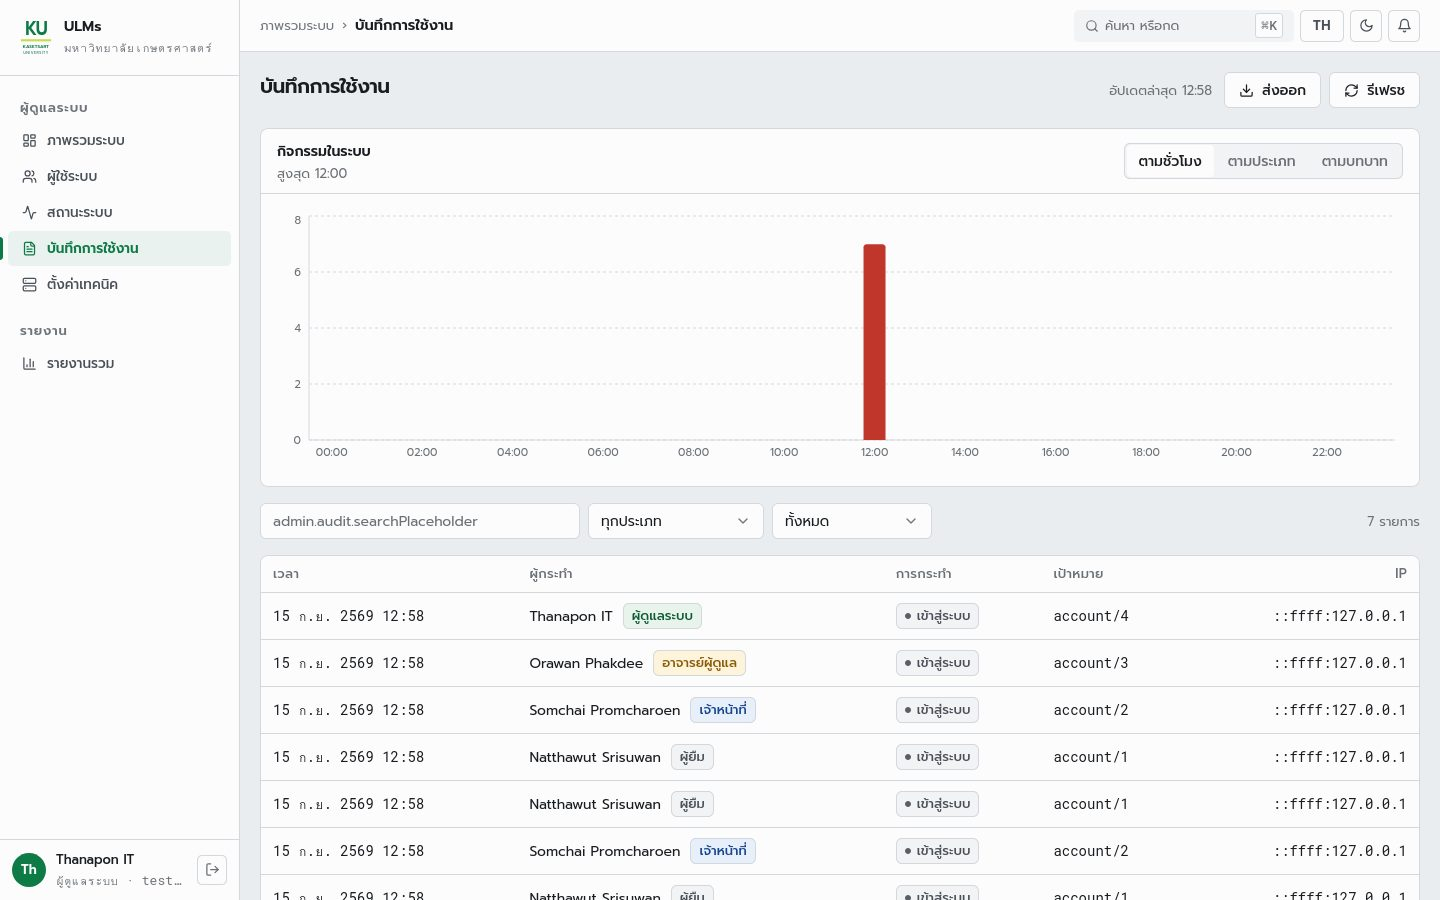
\includegraphics[width=0.95\textwidth, trim={240 240 0 490}, clip]{audit/a-audit}
\caption{หน้าบันทึกการใช้งานของผู้ดูแลระบบ ช่องค้นหาแสดง \code{admin.audit.searchPlaceholder} ตรง ๆ เพราะคีย์นี้ไม่มีในไฟล์ภาษาทั้งไทยและอังกฤษ (F16)
คีย์ที่โค้ดใช้อีก 668 คีย์มีครบทั้งสองภาษา}
\end{figure}

\begin{figure}[H]
\centering
\begin{minipage}[t]{0.49\textwidth}\centering
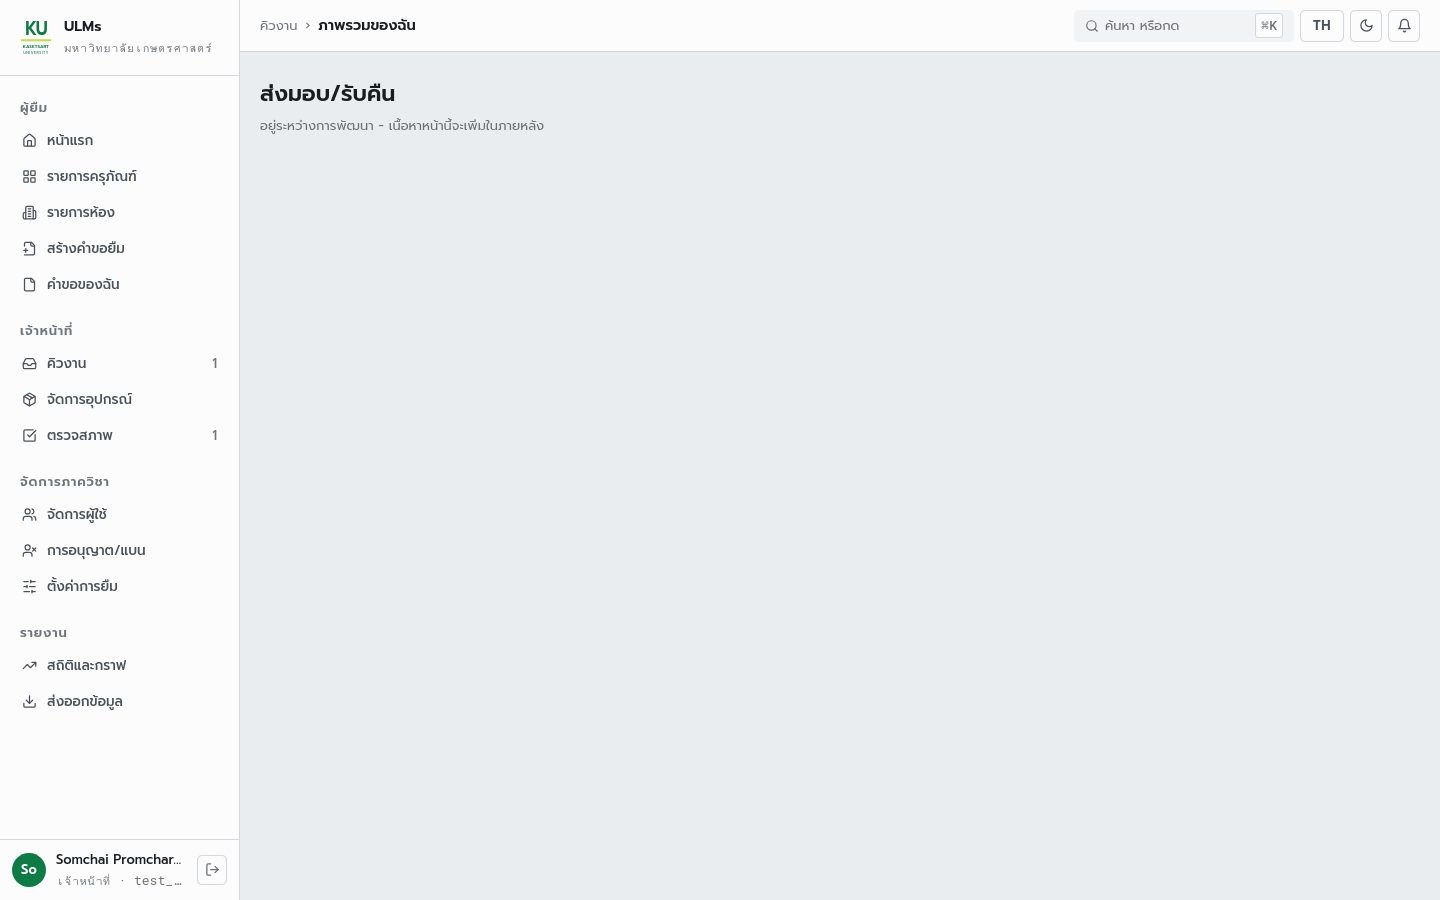
\includegraphics[width=\linewidth, trim={240 450 0 0}, clip]{audit/s-handover-placeholder}\\[2pt]
{\sansall\scriptsize \code{/staff/handover}}
\end{minipage}\hfill
\begin{minipage}[t]{0.49\textwidth}\centering
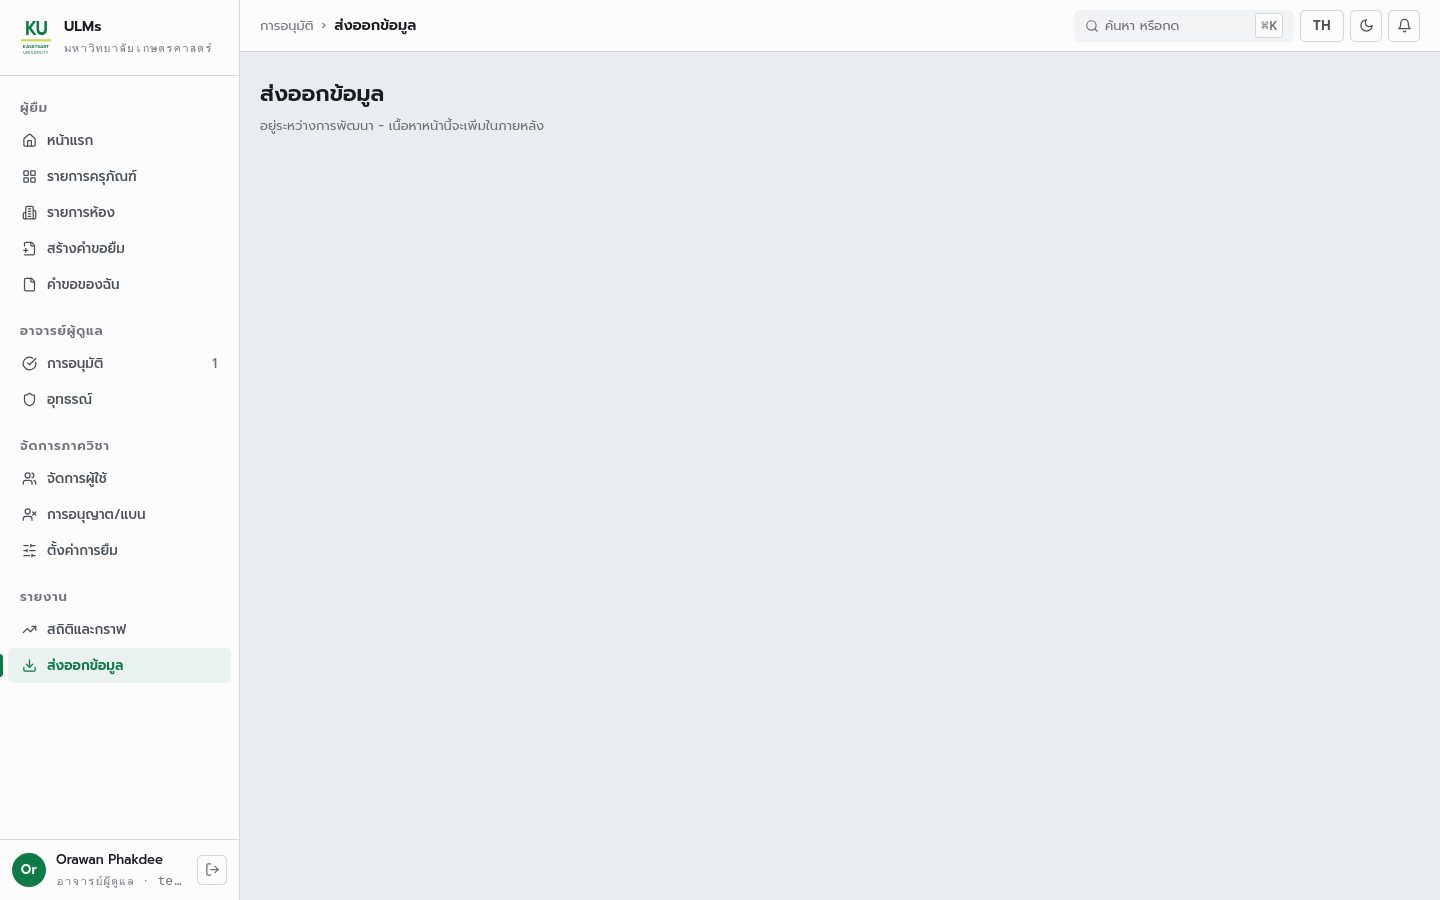
\includegraphics[width=\linewidth, trim={240 450 0 0}, clip]{audit/v-export-placeholder}\\[2pt]
{\sansall\scriptsize \code{/reports/export}}
\end{minipage}
\caption{หน้าที่มีเส้นทางและเมนูแล้วแต่ยังไม่มีเนื้อหา (F18)}
\end{figure}

\begin{table}[H]
\centering\small
\begin{tabular}{L{1.1cm}L{6.9cm}L{6.3cm}}
\toprule
\sansall\bfseries ข้อ & \sansall\bfseries พบ & \sansall\bfseries ที่ \\
\midrule
F18 & หน้ายังว่าง 2 หน้า · ข้อมูลตัวอย่าง: ห้อง 3 หน้า อุทธรณ์ 2 หน้า & \code{use-rooms.ts} · \code{use-appeals.ts} \\
F15 & ค่าหักเครดิตใช้น้ำหนักคงที่ T1=5 T2=10 ไม่ใช่น้ำหนักจริงของแต่ละชิ้น (DSLR ใน \en{seed} คือ 3) & \code{mock-data.ts:632} \code{creditCutOf} \\
F15 & tier ที่ไม่รู้จักถูกเดาเป็น T2 & \code{request.adapter.ts:72} · \code{submitted-requests.store.ts:117} \\
F22 & เมนูฝั่งผู้ยืมของเจ้าหน้าที่และอาจารย์ไม่มี ``ใช้ห้อง'' ``รับของ'' ``การอุทธรณ์'' ทั้งที่ยืมได้ตาม FR-AUTH-04 & \code{constants/navigation.ts} ส่วน \code{staff} และ \code{supervisor} \\
\bottomrule
\end{tabular}
\end{table}

\fstep{คำตัดสิน}
\vbad[ต้องแก้ ระดับต่ำ--กลาง]

% -----------------------------------------------------------------------------
\section{บันทึกการใช้งานเห็นอะไรบ้าง}
\label{sec:auditlog}
% -----------------------------------------------------------------------------
\fmeta{F26}{ตรวจเจอเพิ่ม (พบ 11 ก.ย. ยังไม่แก้)}{BE}

\fstep{แผนว่าไว้}
FR-AUTH-07 บันทึกการเข้าสู่ระบบทุกครั้ง · FR-ADM-05 \emph{``Admin ต้องเห็น Audit Log ของการใช้งานระบบทั้งหมด''}

\fstep{ระบบทำจริง}
หลังรันการตรวจทั้งหมด ฐานข้อมูลทดสอบมีคำขอยืม 15 ใบ แต่ \code{AuditLog} มีแค่สามชนิด

\begin{table}[H]
\centering\small
\begin{tabular}{L{3cm}rL{9cm}}
\toprule
\sansall\bfseries \code{Action} & \sansall\bfseries แถว & \sansall\bfseries มาจาก \\
\midrule
\code{login} & 30 & \code{auth.router.ts:74} \\
\code{update} & 6 & \code{admin.service.ts} (แบน ตั้งค่า) \\
\code{role} & 2 & \code{admin.service.ts} (เปลี่ยนบทบาท) \\
ส่งคำขอ อนุมัติ จัดเตรียม ส่งมอบ ตรวจสภาพ ลงทะเบียน & \textcolor{bad}{0} & \code{loan} \code{approval} \code{inspection} \code{item} ไม่เรียก \code{audit.record} เลย \\
\bottomrule
\end{tabular}
\end{table}

\fstep{คำตัดสิน}
FR-AUTH-07 \vok[ตรงแผน] \quad FR-ADM-05 \vbad{} ถ้ามีข้อพิพาทว่าใครอนุมัติหรือใครให้ระดับความเสียหาย ย้อนดูจากบันทึกไม่ได้
\fstep{ข้อเสนอ}
BE เรียก \code{audit.record} ในคำสั่งที่เปลี่ยนสถานะทั้งหมดของ \code{loan} \code{approval} \code{inspection} และคำสั่งสร้าง/แก้ของ \code{item}

% -----------------------------------------------------------------------------
\section{test ที่มีอยู่พิสูจน์อะไรได้ และอะไรยังไม่ได้}
\label{sec:tests}
% -----------------------------------------------------------------------------
\fmeta{F21}{รันทุกชุดบน \code{b1bca77}}{ทีม test · BE · FE}

\begin{table}[H]
\centering\small
\begin{tabular}{L{5.6cm}L{2.4cm}L{6.3cm}}
\toprule
\sansall\bfseries ชุด & \sansall\bfseries ผล & \sansall\bfseries ครอบคลุม \\
\midrule
\en{backend} \code{npm test} (ฐานข้อมูลแยก) & 266/266 · 24 ชุด & \en{unit} ของ \en{service} ส่วนใหญ่ \\
\en{backend} \code{test:item} & 13/13 & จัดการอุปกรณ์ (ข้อมูลจำลอง ไม่ใช้ฐานข้อมูล) \\
\en{backend} \code{test:admin} & 16/16 & จัดการผู้ใช้ \\
\en{frontend} \code{typecheck} & ผ่าน & หลัง \code{npm ci} (โมดูลในเครื่องค้าง ไม่ใช่บั๊ก) \\
\en{frontend} \code{vitest} & 33/33 & catalog inventory หน้าผู้ใช้ของผู้ดูแล \\
\en{frontend} \code{test:ac} & 49/49 & ฟังก์ชันกฎธุรกิจ (มีข้อ 2.6 ที่ใช้กฎห้องเก่า) \\
\en{frontend} \code{lint} & 0 error · 7 warning & --- \\
\en{Playwright} \en{e2e} & 10 ผ่าน · 1 ข้าม & ผู้ดูแลระบบ และหน้ารายการอุปกรณ์ \\
\bottomrule
\end{tabular}
\end{table}

\begin{warnbox}[title={ทุกชุดผ่าน แต่ไม่มีชุดใดแตะวงจรยืม}]
ไม่มี \en{test} ของ \code{loan} \code{approval} \code{inspection} ทั้ง \en{unit} และ \en{e2e}
ข้อผิดพลาดใน F04 F10 F12 F17 F23 F24 จึงผ่าน \en{test} ทั้งหมดได้ สถานการณ์ S1--S5 ในเล่มนี้เขียนเป็นสคริปต์ที่รันซ้ำได้แล้ว
ใช้เป็นต้นแบบกรณีทดสอบได้ทันที โดยแปลงค่าที่ ``ผิด'' ในตารางให้เป็นค่าที่ต้องการ

\smallskip คำตัดสิน \vbad{}
\end{warnbox}

\clearpage
% =============================================================================
\part{สิ่งที่ต้องทำ แยกตามเจ้าของงาน}
% =============================================================================

\textbf{เรียงตามลำดับที่ควรทำในแต่ละกลุ่ม เลขข้อชี้กลับไปยังหลักฐาน ระดับ: สูง = วงจรยืมหรือความถูกต้องของข้อมูลพัง · กลาง = ขัดแผน · ต่ำ = ความเรียบร้อย}

\section{SA --- ข้อความใน SRS/SDS ที่ต้องแก้ และเรื่องที่ต้องตัดสิน}

\begin{table}[H]
\centering\small
\begin{tabular}{L{1cm}L{9.4cm}L{2.2cm}L{1.6cm}}
\toprule
\sansall\bfseries ลำดับ & \sansall\bfseries งาน & \sansall\bfseries ข้อ & \sansall\bfseries ระดับ \\
\midrule
1 & ตัดสินจุดกันของ = ตั้งแต่ส่งคำขอ แก้ FR-APV-05 และข้อความในข้อเสนอ & F04 & สูง \\
2 & ยืนยันลำดับรับของ: ผู้ยืมยืนยัน+รูป แล้วเจ้าหน้าที่ส่งมอบ (คง FR-PKP-02/03) & F05c & สูง \\
3 & แก้ FR-RTN-01 เจ้าหน้าที่ถ่ายรูปตอนรับคืน & F05b & สูง \\
4 & แก้ FR-REQ-08 เป็น 30 นาที × 6 ช่อง · FR-EQP-04 ความยาวช่องเป็นค่ากลาง จองทั้งห้อง & F02 F10 & สูง \\
5 & เพิ่ม FR ปฏิทินช่วงวันสำหรับอุปกรณ์ในหมวด BRW & F01 & สูง \\
6 & แก้ FR-EQP-03, FR-EQP-06, FR-PKP-01 ตาม T1 ไม่มี serial · ตัด FR-PKP-04 & F05d F06 & กลาง \\
7 & เพิ่ม FR ผู้อนุมัติ T3 = เจ้าหน้าที่ & F11 & กลาง \\
8 & ตัดสิน FR-CRD-06 (เครดิตคำนวณจากโทษที่ยัง \en{active}) · แก้ SDS v1.1 ที่เขียนการระงับการยืมไว้ตามโค้ด & F17 & กลาง \\
9 & ตัดสินการต่ออายุ D2--D3 และ T3 (ค้างจาก SDS v1.1) & F20 & กลาง \\
10 & ใช้ตาราง ``หลังแก้'' ในหัวข้อ~\ref{sec:roles} เป็นเกณฑ์ตรวจความสามารถใหม่ & F19 & กลาง \\
\bottomrule
\end{tabular}
\end{table}

\section{BE-lead --- โครงสร้างฐานข้อมูล}

\begin{table}[H]
\centering\small
\begin{tabular}{L{1cm}L{9.4cm}L{2.2cm}L{1.6cm}}
\toprule
1 & \code{RoomInfo.Capacity} (และเวลาเปิด--ปิดถ้าไม่ใช้ค่ากลาง) & F02 & สูง \\
2 & ที่เก็บเหตุผลการปฏิเสธแยกจากเหตุผลผู้ยืม (ถ้าเลือกเพิ่มคอลัมน์) & F17 & ต่ำ \\
3 & ถ้าเลือกเก็บสิทธิ์ยืมระดับประเภทแทนระดับชิ้น & F24 & กลาง \\
\bottomrule
\end{tabular}
\end{table}
ไม่ต้องเพิ่มตาราง slot (หัวข้อ~\ref{sec:slots}) ไม่ต้องเพิ่มสถานะส่งมอบ (หัวข้อ~\ref{sec:pickupphoto}) และไม่ต้องเพิ่มตารางรูป

\section{Back-End}

\begin{table}[H]
\centering\small
\begin{tabular}{L{1cm}L{9.4cm}L{2.2cm}L{1.6cm}}
\toprule
1 & ฟังก์ชัน ``ว่างในช่วง'' ชุดเดียว ใช้ทุกตัวนับ + \en{query} ปฏิทินรายวัน & F04 F01 F09 & สูง \\
2 & \code{allocate} ห้ามเปลี่ยนเครื่อง T2 & F12 & สูง \\
3 & คำสั่งผู้ยืมยืนยันรับ+รูป · \code{confirmPickup} ต้องมีรูปก่อน · \code{requestUpload} ตามจุดประสงค์ & F05c F13 & สูง \\
4 & \code{recordReturn} รับรูป & F05b & สูง \\
5 & กฎห้องใน \code{loan.create} + \en{query} \code{roomSlots} & F03 F10 & สูง \\
6 & เปิดสิทธิ์จองห้อง · \code{createUnit} นับเลขต่อและคัดลอกสิทธิ์ · T1 ไม่บังคับ serial & F23 F24 F06 & สูง \\
7 & ลบการแบนการยืมที่ไม่มีในแผน · ป้ายสถานะไม่ใช้ ``ถูกระงับ'' · ไม่เขียนทับเหตุผลผู้ยืม & F17 F25 & กลาง \\
8 & \en{router} อุทธรณ์ & F18 F19 & กลาง \\
9 & \code{audit.record} ในวงจรยืม & F26 & กลาง \\
10 & \code{createType} ตรวจหน่วยงาน · ตัดสถานะ \code{preparing} & F13 F08 & ต่ำ \\
\bottomrule
\end{tabular}
\end{table}

\section{Front-End}

\begin{table}[H]
\centering\small
\begin{tabular}{L{1cm}L{9.4cm}L{2.2cm}L{1.6cm}}
\toprule
1 & ต่อ \code{loan.create} \code{loan.cancel} \code{loan.requestExtension} เลิกใช้ที่เก็บในหน่วยความจำ & F07 & สูง \\
2 & ใช้สัญญาที่ \en{generate} จาก \en{backend} & F14 & สูง \\
3 & หน้าลงทะเบียนอุปกรณ์/ห้อง ครบสามขั้น + ปุ่มเพิ่มจำนวน & F06 & สูง \\
4 & ปฏิทินช่วงวันในหน้าสร้างคำขอ ป้ายของว่างใช้ช่วงที่เลือก & F01 F09 & สูง \\
5 & หน้ารับของต่อคำสั่งยืนยันรับ · ลบปุ่มขอเปลี่ยนชิ้น · คิวงานแสดงสถานะยืนยัน & F05c F05d & สูง \\
6 & รับคืนพร้อมถ่ายรูป · หน้าตรวจสภาพเทียบรูปก่อน/หลัง & F05b & สูง \\
7 & หน้าห้องใช้ข้อมูลจริง ลบค่าคงที่ห้องเก่าและแก้ \code{test:ac} 2.6 & F03 F10 F18 & กลาง \\
8 & หน้าอุทธรณ์สองหน้าต่อ \en{router} ใหม่ & F18 & กลาง \\
9 & น้ำหนักเครดิตจริง · ไม่เดา T2 · แสดง \code{returned} เป็นรอตรวจสภาพ & F15 F08 & ต่ำ \\
10 & คีย์ข้อความที่หาย · เมนูฝั่งผู้ยืมของเจ้าหน้าที่/อาจารย์ · หน้าส่งมอบและส่งออกที่ว่าง · เอาหน้า ``การอนุญาต/แบน'' ออก & F16 F22 F18 F17 & ต่ำ \\
\bottomrule
\end{tabular}
\end{table}

\clearpage
% =============================================================================
\appendix
\part*{ภาคผนวก}
\addcontentsline{toc}{part}{ภาคผนวก}
% Thai letters for appendix numbers instead of article's A B C (same as trpc-guide.tex)
\makeatletter
\newcommand{\thaialph}[1]{\ifcase\value{#1}\or ก\or ข\or ค\or ง\or จ\or ฉ\fi}
\makeatother
\renewcommand{\thesection}{\thaialph{section}}

\section{FR ที่มีปัญหาหรือต้องแก้}
\label{app:fr}

เฉพาะ FR ที่ผลตรวจในเล่มนี้แตะถึง จาก 86 ข้อใน SRS v1.0 ช่อง ``ทาง'' บอกว่าต้องแก้ระบบให้ตรง FR หรือแก้ FR ให้ตรงข้อตัดสิน

{\small
\begin{longtable}{L{1.9cm}L{1cm}L{7.3cm}L{1.9cm}L{1.9cm}}
\toprule
\sansall\bfseries FR & \sansall\bfseries ระดับ & \sansall\bfseries ปัญหา & \sansall\bfseries ข้อ & \sansall\bfseries ทาง \\
\midrule
\endhead
FR-EQP-01 & สูง & ไม่มีหน้าจอลงทะเบียน · สิทธิ์ต้องตั้งแยก & F06 & แก้ระบบ \\
FR-EQP-03 & สูง & T1 นับจำนวนแต่ \en{backend} บังคับ serial · ข้อความ ``ผูก serial'' ขัดข้อตัดสิน & F06 & แก้ทั้งคู่ \\
FR-EQP-04 & สูง & ไม่มีที่นั่ง เวลาเปิด · ความยาวช่องเป็นค่ากลางแล้ว & F02 & แก้ทั้งคู่ \\
FR-EQP-06 & กลาง & ประวัติรายชิ้น T1 ทำไม่ได้เมื่อไม่มี serial & F06 & แก้ FR \\
FR-EQP-07 & สูง & วันที่พร้อมให้ยืมคิดจากจำนวน ``ตอนนี้'' & F04 F01 & แก้ระบบ \\
FR-EQP-08 & กลาง & จำหน่ายของ \code{NOT\_IMPLEMENTED} & F19 & แก้ระบบ \\
FR-BRW-03 & สูง & จำนวนคงเหลือสองหน้าจอไม่เท่ากัน & F04 & แก้ระบบ \\
FR-BRW-05 & สูง & ช่องเวลาห้องเป็นค่าสมมติ & F03 & แก้ระบบ \\
FR-REQ-01--10 & สูง & ปุ่มส่งคำขอไม่ถึง \en{backend} & F07 & แก้ระบบ \\
FR-REQ-03 & สูง & หน้าจอตรวจของคงเหลือกับจำนวนตอนนี้ & F09 & แก้ระบบ \\
FR-REQ-07 & สูง & serial T2 ที่อนุมัติถูกเปลี่ยนตอนจัดเตรียมได้ & F12 & แก้ระบบ \\
FR-REQ-08 & สูง & รายชั่วโมง 2 สล็อต ขัดข้อตัดสิน · \en{backend} ไม่บังคับกฎ & F10 & แก้ทั้งคู่ \\
FR-RSV-02 & กลาง & \en{backend} รับจองห้องล่วงหน้า & F10 & แก้ระบบ \\
FR-APV-05 & สูง & จุดกันของขัดกับ SDS และข้อเสนอ & F04 & แก้ FR \\
FR-PKP-01 & สูง & เลือก serial T1 ขัดข้อตัดสิน & F06 & แก้ FR \\
FR-PKP-02/03 & สูง & ผู้ยืมยืนยัน/อัปโหลดรูปไม่ได้ & F05c & แก้ระบบ \\
FR-PKP-04 & กลาง & ขัดข้อตัดสินเปลี่ยนนอกระบบ & F05d & แก้ FR \\
FR-RTN-01 & สูง & ผู้ยืมถ่ายรูปคืน ขัด BPMN และข้อเสนอ & F05b & แก้ FR \\
FR-RTN-02 & สูง & ไม่มีรูปให้เทียบ & F05b F05c & แก้ระบบ \\
FR-APL-01--06 & สูง/กลาง & ไม่มี \en{router} อุทธรณ์ & F18 & แก้ระบบ \\
FR-CRD-06 & สูง & เครดิตถูกลบตรง ไม่คำนวณจากโทษที่ \en{active} & F17 & ต้องตัดสิน \\
FR-CRD-08 & สูง & มีการแบนการยืมที่ SRS ไม่มี (โทษตามแผนมีผลผ่านแถบเครดิตเท่านั้น) & F17 F25 & แก้ระบบ \\
FR-AUTH-05 & สูง & \code{createType} ไม่ตรวจหน่วยงาน & F13 & แก้ระบบ \\
FR-ADM-05 & กลาง & บันทึกไม่มีการยืม อนุมัติ ตรวจ & F26 & แก้ระบบ \\
FR-RNW-04/06 & กลาง/สูง & การต่ออายุ T3 และ D2--D3 ต่างจากโค้ด & F20 & ต้องตัดสิน \\
\bottomrule
\end{longtable}
}

\section{ผลรันสถานการณ์และภาพหน้าจอฉบับเต็ม}
\label{app:runs}

\begin{table}[H]
\centering\small
\begin{tabular}{L{2.8cm}rL{7.2cm}L{3.2cm}}
\toprule
\sansall\bfseries สถานการณ์ & \sansall\bfseries ครั้ง & \sansall\bfseries ทำอะไร & \sansall\bfseries ใช้ในหัวข้อ \\
\midrule
S1 \code{s1\_counters} & 37 & T1 3 ชิ้น เดินทุกสถานะ อ่านตัวนับ 3 จุดหลังทุกขั้น & \ref{sec:counter} \ref{sec:calendar} \\
S2 \code{s2\_overlap} & 14 & ของชิ้นเดียว 5 ช่วงเวลา สองผู้ยืม & \ref{sec:overlap} \\
S3 \code{s3\_rooms} & 13 & ห้องใหม่ สิทธิ์จอง 8 คำขอที่ผิดกฎต่างกัน & \ref{sec:slots} \ref{sec:roomelig} \\
S4 \code{s4\_handover} & 20 & T2 สองเครื่อง อนุมัติ จัดเตรียมผิดเครื่อง ส่งมอบ ตรวจสภาพ สิทธิ์ 403 & \ref{sec:serialab} \ref{sec:handover} \ref{sec:scope} \\
S5 \code{s5\_registration} & 25 & ลงทะเบียนตาม tier จำนวน serial และการเพิ่มชิ้น & \ref{sec:register} \\
\bottomrule
\end{tabular}
\end{table}

ภาพหน้าจอ 16 ภาพ (\code{docs/figures/audit/}): \rbor{} \code{b-catalog} \code{b-detail-t1} \code{b-request} \code{b-request-mobile}
\code{b-rooms} \code{b-room-booking} \code{b-pickup} \code{b-my-loans} · \rstf{} \code{s-queue} \code{s-inventory} \code{s-inspection}
\code{s-handover-placeholder} · \rsup{} \code{v-approvals} \code{v-appeals-mock} \code{v-export-placeholder} · \radm{} \code{a-audit}
ข้อมูลที่สคริปต์ใส่ไว้ก่อนถ่าย (คำขอ T1 ที่จัดเตรียมแล้ว ของ T0 ที่รับคืนแล้ว คำขอ T2 รออนุมัติ) อยู่ใน \code{results/screens.json}

\section{วิธีรันการตรวจซ้ำ}
\label{app:howto}

ต้องมี \en{container} Postgres ของทีมชื่อ \code{postgres} และ \code{backend/.env} ตาม \code{backend/README.md}
ฐานข้อมูลที่ใช้ตรวจแยกจากฐาน \code{app} ปกติ ไม่ทับข้อมูลเดิม

\begin{lstlisting}[language={}]
# 1. fresh audit database (backend must be stopped first)
docker exec postgres psql -U postgres -c "DROP DATABASE IF EXISTS ulms_audit WITH (FORCE)" \
                                      -c "CREATE DATABASE ulms_audit"
cd backend
export DATABASE_URL="postgresql://postgres:<password>@localhost:5432/ulms_audit"
npx prisma migrate deploy && npm run seed
npm run start                                   # :3000, keep running

# 2. frontend
cd ../frontend && npm ci && npm run dev         # :5173

# 3. evidence, in this order (screens first, or AUDIT-* items show up in the catalogue shots)
python3 -m venv /tmp/audit-venv && /tmp/audit-venv/bin/pip install playwright requests
/tmp/audit-venv/bin/playwright install firefox
/tmp/audit-venv/bin/python docs/audit/capture_screens.py
/tmp/audit-venv/bin/python docs/audit/api_scenarios.py        # or: ... api_scenarios.py s1 s3

# 4. team test suites (backend on a separate database)
DATABASE_URL=".../ulms_test" npm test && npm run test:item && npm run test:admin
cd frontend && npm run typecheck && npm test && npm run test:ac && npm run lint
cd .. && npm ci && npx playwright install chromium && npx playwright test

# 5. this document
cd docs && latexmk web-audit.tex && cp build/web-audit.pdf report/
\end{lstlisting}

ตัวเลขในเนื้อความทุกตัวมาจาก \code{docs/audit/results/*.json} ถ้ารันซ้ำบน \en{commit} ใหม่แล้วค่าเปลี่ยน ต้องแก้ตารางในเล่มตาม
ชื่อของที่สคริปต์สร้างมีรหัสรอบ (เช่น \code{AUDIT-S1 ... 09151258}) จึงรันซ้ำบนฐานเดิมได้โดยไม่ชนกัน

\section{รายการแก้ SRS/SDS รายข้อ}
\label{app:srs}

\begin{longtable}{L{1.9cm}L{6.1cm}L{6.3cm}}
\toprule
\sansall\bfseries ข้อ & \sansall\bfseries ข้อความเดิม & \sansall\bfseries ข้อความที่เสนอ \\
\midrule
\endhead
FR-REQ-08 & สำหรับคำขอ T3 Borrower ต้องเลือกสล็อตเวลาเป็นรายชั่วโมง จองพร้อมกันได้สูงสุด 2 สล็อต
          & สำหรับคำขอ T3 Borrower ต้องเลือกช่องเวลาช่องละ 30 นาที ต่อเนื่องกันไม่เกิน 6 ช่องต่อการจองหนึ่งครั้ง \\
FR-EQP-04 & ... พร้อมกำหนดจำนวนที่นั่ง ความยาวสล็อต และช่วงเวลาเปิดใช้
          & ... พร้อมกำหนดจำนวนที่นั่งและช่วงเวลาเปิดใช้ ความยาวช่องเวลาเป็นค่ากลาง 30 นาที การจองเป็นแบบทั้งห้อง \\
FR-EQP-03 & สำหรับอุปกรณ์ T1 ระบบต้องรองรับการนับเป็นจำนวน (quantity) และผูก Serial Number ตอน allocation
          & สำหรับอุปกรณ์ T1 ระบบต้องรองรับการนับเป็นจำนวน (quantity) โดยไม่ต้องมี Serial Number \\
FR-EQP-06 & ... รายชิ้นสำหรับ T1-T2 & ... รายชิ้นสำหรับ T2 \\
FR-PKP-01 & Staff ต้องสามารถเลือก Serial Number ของอุปกรณ์ T1 ตอนจัดเตรียม และบันทึกลงในระบบ
          & ตัดข้อนี้ (T1 ไม่มี serial) \\
FR-PKP-02 & Borrower ต้องยืนยันการรับอุปกรณ์และตรวจสอบ Serial Number ก่อนกดยืนยัน
          & คงเดิม และเพิ่ม: Staff บันทึกการส่งมอบได้หลัง Borrower ยืนยันแล้วเท่านั้น \\
FR-PKP-04 & สำหรับ T1 Borrower ต้องสามารถขอเปลี่ยนอุปกรณ์ตอนรับได้หากพบปัญหา
          & ตัดข้อนี้ หรือ: การเปลี่ยนชิ้น T1 ทำที่จุดบริการโดยไม่บันทึกในระบบ \\
FR-RTN-01 & Borrower ต้องสามารถแจ้งคืนผ่านระบบพร้อมอัปโหลดรูปถ่ายตอนคืน
          & Staff ต้องบันทึกการรับคืนพร้อมอัปโหลดรูปถ่ายอุปกรณ์ตอนคืน \\
FR-APV-05 & เมื่อคำขอได้รับการอนุมัติ ระบบต้องสร้าง Allocation ...
          & ระบบต้องกันอุปกรณ์ในช่วงเวลาที่ขอตั้งแต่รับคำขอ และคงไว้เมื่ออนุมัติ พร้อมกำหนด pickup\_deadline 24 ชั่วโมง \\
ใหม่ BRW & --- & สำหรับ T0--T2 ระบบต้องแสดงปฏิทินให้เลือกช่วงวันยืม วันที่อุปกรณ์ว่างไม่พอต้องเลือกไม่ได้ \\
ใหม่ APV & --- & คำขอ T3 ต้องได้รับการอนุมัติจาก Staff ของหน่วยงานเจ้าของสถานที่ \\
FR-RNW-04/06 & (ค้างจาก SDS v1.1) & รอที่ประชุมตัดสิน ตามรายงานความก้าวหน้าครั้งที่ 3 \\
\bottomrule
\end{longtable}

SDS ที่ต้องแก้ตาม: ตารางสถานะ (ลำดับ ผู้ยืมยืนยัน $\to$ ส่งมอบ) · กรณีใช้งานส่งคำขอ (จุดกันของ) · รายการ \en{procedure} (\code{confirmReceipt} \code{roomSlots} \code{availabilityCalendar} \code{setRoomEligibility})

\section{อภิธานศัพท์}

{\small
\begin{longtable}{L{3.6cm}L{10.7cm}}
\toprule
\sansall\bfseries คำ & \sansall\bfseries ความหมายในเล่มนี้ \\
\midrule
\endhead
T0 T1 T2 T3 & ระดับอุปกรณ์ตามมูลค่า: ยืมง่าย · ยืมได้ · ยืมยาก (อาจารย์อนุมัติ) · ของติดที่ คือห้อง \\
D0--D3 & แถบเครดิตของผู้ยืม กำหนดจำนวนวันยืมสูงสุดและผู้อนุมัติ \\
\code{Reservations} & ตารางคำขอ หนึ่งแถวต่อหนึ่งชิ้น สถานะ \code{Pending Approved Rejected Canceled} \\
\code{UsageLog} & ตารางการยืมจริง เริ่มตอนจัดเตรียม สถานะ \code{Prepared Lended Returned Inspected} \\
\code{Eligibility} & แถวที่บอกว่าบทบาทใดในหน่วยงานใดยืมชิ้นนี้ได้ ไม่มีแถว = ไม่มีใครยืมได้ \\
\code{BufferTime} & วันเตรียมของก่อนและหลังการยืม นับรวมตอนตรวจการจองซ้อน \\
\en{procedure} & คำสั่งหนึ่งตัวของ \en{tRPC} เช่น \code{loan.create} \\
\en{seed} & สคริปต์ใส่ข้อมูลตั้งต้น (บัญชีทดสอบ อุปกรณ์ 4 ประเภท 15 ชิ้น) \\
ข้อมูลตัวอย่าง (\en{mock}) & ข้อมูลที่เขียนไว้ในโค้ดหน้าจอ ไม่ได้มาจากฐานข้อมูล \\
ช่องเวลา (slot) & ช่วง 30 นาทีที่จองห้องได้ ตามข้อตัดสินของทีม \\
S1--S5 & สถานการณ์ทดสอบในภาคผนวก ข \\
\bottomrule
\end{longtable}
}

\vfill
{\footnotesize\color{muted}\sansall ที่มาของตัวเลขและภาพทั้งหมด: \code{docs/audit/api\_scenarios.py} และ \code{docs/audit/capture\_screens.py}
รันบน \code{b1bca77} เมื่อ 15 ก.ย. 2569 ผลดิบอยู่ใน \code{docs/audit/results/} ถ้าโค้ดเปลี่ยนแล้วรันใหม่ ตัวเลขในเล่มต้องตามไปแก้}

\end{document}
